\documentclass[]{ctexbook}

\usepackage[a4paper,left=2cm,right=2cm,top=2cm,bottom=2cm]{geometry}
\usepackage[dvipsnames]{xcolor}
\usepackage[most]{tcolorbox}
\usepackage{amsmath}
\usepackage{listings}
\usepackage{pdfpages}
\usepackage{hyperref} 

\definecolor{codegreen}{rgb}{0,0.6,0}
\definecolor{codegray}{rgb}{0.5,0.5,0.5}
\definecolor{codepurple}{rgb}{0.58,0,0.82}
\definecolor{backcolour}{rgb}{0.95,0.95,0.92}

\lstset{
    backgroundcolor=\color{backcolour},
    commentstyle=\color{codegreen},
    keywordstyle=\color{magenta},
    numberstyle=\tiny\color{codegray},
    stringstyle=\color{codepurple},
    basicstyle=\ttfamily\fontsize{9}{11}\selectfont,  % 调整这里的字体大小和行高
    numbers=left,
    stepnumber=1,
    numbersep=5pt,
    abovecaptionskip=1em,
    breaklines=true,  
    breakatwhitespace=true,  
    captionpos=b,  
    keepspaces=true,  
    showspaces=false,  
    showstringspaces=false,
    showtabs=false,
    tabsize=2,
}

\newcommand{\citebox}[1]{
    \begin{center}
    \begin{tcolorbox}[colback=gray!10,%gray background
                      colframe=black,% black frame colour
                      width=15cm,% Use 8cm total width,
                      arc=1mm, auto outer arc,
                      boxrule=0.5pt,
                     ]
    #1
    \end{tcolorbox}
    \end{center}
}


\title{COMPSCI 701 Note}
\author{Bo Pang/庞礴}
\date{Last Update: \today}

\ctexset{
	part = {
		format+=\heiti
	},
    part/name = {第, 编},
    part/number = {\Chinese{part}},
    chapter/name = {Chapter},
    chapter/number = { \arabic{chapter}},
    chapter = {
		format+=\heiti
	},
    section = {
		format+=\heiti
	},
	subsection = {
		format+=\heiti
	},
	subsubsection = {
		format+=\heiti
	},
    paragraph = {
		format+=\heiti
	}
}


\begin{document}
\maketitle
\tableofcontents

\part{创建可维护的程序、程序的可理解性}

\chapter{Creating Maintainable Software}

产品的\textbf{生命周期成本}是指产品生命周期内(从最初构思conceived到退役retired)的所有费用
(以金钱、精力、时间或其他方式衡量)的总和。\textbf{软件维护}是指保持软件产品有用性的活动。
研究表明,产品生命周期内的大部分费用发生在产品首次交付之后。所以,减少维护活动的成本
将大大降低软件产品的生命周期成本。软件产品的\textbf{可维护性}是指对其进行维护活动的难易程度。
可维护性是软件\textbf{质量}的一个方面。

\section{Maintainablity}
\paragraph{可维护性(Maintainability)}是产品的特性或属性,它影响维护活动开展的难易程度。
代码的设计和编写方式对该属性有很大影响。它是对产品进行维护活动的有效性(effectiveness)和效率(efficiency)。

而维护是产品交付后进行的活动。通常描述为:
\begin{itemize}
    \item 纠正性 corrective - 消除缺陷
    \item 适应性 adaptive - 改变产品以适应变化的环境
    \item 预防性 preventative - 改进质量的某些方面
    \item 完善性 perfective - 改进其实用性的某些方面,包括增加新功能
\end{itemize}

许多活动都在交付前进行。

\paragraph{Quality} For developers, quality means be more efficient at creating software. Ex: cheaper, produce, develop, fix faster\dots

\citebox{A quality attribute is a [quantifiable] or testable property of a system that is used to indicate how well the system satisfies the needs of its stakeholders}

是软件质量的一个方面。 In this course, we define maintainablity including these \textbf{independent} sub-attributes: \textbf{Comprehensibility, Alterability, Testability}.

\citebox{
    The degree of effectiveness and efficiency with which maintenance activities can be carried out on the product. It includes these independent sub-attributes:
    \begin{itemize}
        \item Comprehensibility (Analysability) -- Degree of effectiveness and efficiency with which the implementation can be understood in order to conduct maintenance activities with confidence
        \item Alterability (Modifiability) -- degree to which a product or system can be effectively and efficiently changed without introducing defects or degrading existing product quality.
        \item Testability -- degree of effectiveness and efficiency with which test criteria can be established for a system, product or component and tests can be performed to determine whether those criteria have been met.
    \end{itemize}
    The capability to smoothly and successfully perform maintenance tasks on the given item is defined by its maintainability. This encompasses several distinct characteristics:
    \begin{itemize}
        \item Understandability (Analysability) -- The ease and quickness with which the internal workings of the system can be grasped to confidently undertake maintenance tasks.
        \item Adaptability (Modifiability) -- The extent to which changes can be made to a system or product both swiftly and effectively without causing issues or diminishing its current quality.
        \item Examinability -- The ease and precision with which testing benchmarks can be defined and executed for any system, product, or part, confirming the fulfillment of set standards.
    \end{itemize}
}

Note that: 1. They are independent: when we talk about alterability, we must assume comprehensibility is OK. 2. Maintenance happens even before delivery.

\section{Comprehensibility}



\subsection{Program Comprehension Model}

有些因素与与我们为使代码易于理解而做出的决定无关,例如:使用未知的语言,阅读代码的人的水平\dots 我们需要一种“剔除”这些因素的方法,以便在评估与可理解性相关的决策时,不受试图理解代码的人的影响。为此,我们需要能够描述理解的"含义",这就是\textbf{程序理解模型(Program Comprehension Model)}。

作用:PCM explains how comprehension happens, the main components, processes, and interactions between them. It provides a systematic way for making a decision between choices relating to writing comprehensive code.

\begin{figure}[h]
    \centering
    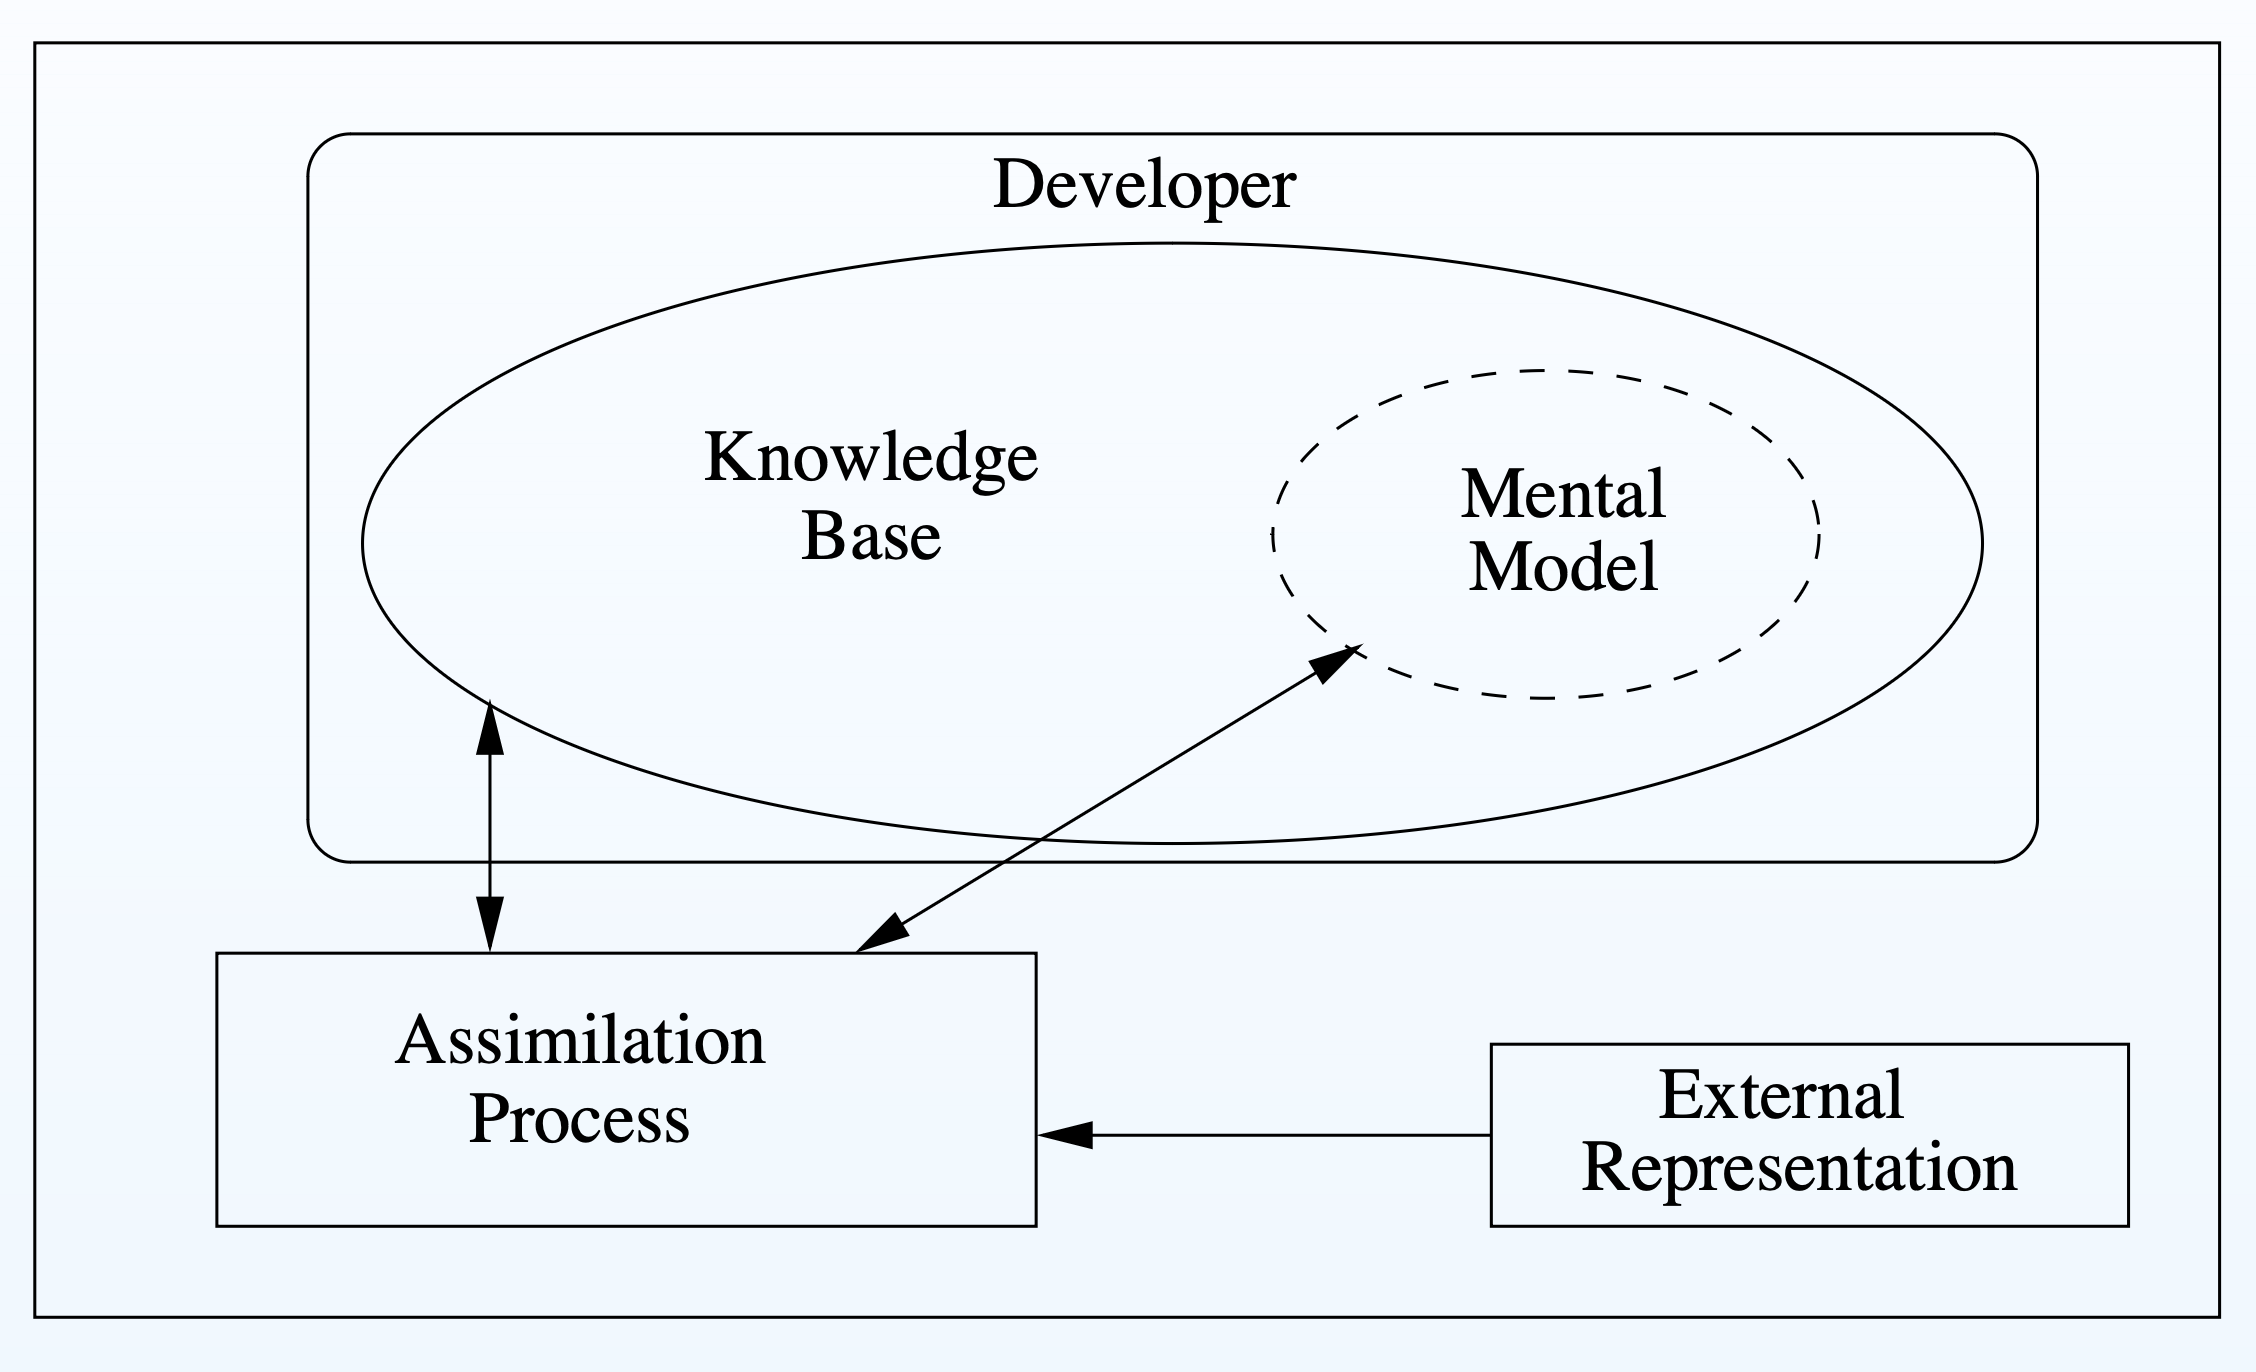
\includegraphics[width=8cm]{res/PCM.png}
    \caption{PCM by Michael}
\end{figure}

\begin{itemize}
    \item External Representation: e.g. source code, docs, peers\dots
    \item Knowledge Base: relevant knowledge that developers have already known, e.g. programming lang, domain knowledge
    \item Mental Model: current understanding, e.g. know parts, hypotheses
    \item Assimilation Process(内化过程): how to use all information to update the mental model, e.g. generation and verification of hypotheses
\end{itemize}

\subsection{可理解性与维护的关系}
可理解性关乎于开发者如何有效和高效地理解代码,以便有信心地进行维护活动。代码的可理解性与其维护性是紧密关联的。代码越容易理解,维护成本就越低,从而提高了代码的长期可维护性。
要提高代码的维护性,我们需要确保代码更容易、更快速且花费更少的精力去理解。

\subsection{如何评估可理解性?}

\paragraph{理解的有效性(Effectiveness)与效率(Efficiency)}要解释对一个实现的理解的有效性和效率,可以通过理解模型来实现,特别是考虑到同化过程的效果。

\paragraph{同化过程的有效性与效率}它取决于从知识库 (KB)、心智模型 (MM) 和外部表示 (ER) 中获取信息的效率和有效性。

\paragraph{信息的来源和理解难度的关系}信息的位置或来源对于理解来说非常关键。信息在心智模型、知识库还是外部表示中,这决定了理解的难度。

\section{Alterability}
\paragraph{可变性}是在不引入缺陷或降低现有产品质量的情况下,对产品或系统进行有效地和高效地改变的程度。

\subsection{Change Cases}
\paragraph{更改案例}描述了系统的潜在新需求或对现有需求的修改。它们的目的是预测和捕捉可能的更改,并指导系统的实现方式,以降低如果需要进行这些更改时的成本。

它们包括案例发生的可能性(Liklihood)和潜在的影响程度(Impact),可以视为系统演进的“用例”。

\subsection{评估可变性}
首先,需要确定实现应当适应哪些更改案例。
其次,针对这些更改案例评估实现。这意味着要查看系统或产品如何响应或适应这些特定的更改案例。

但请注意,有效和高效 "不包括与理解相关的成本
有些代码可能 "难以 "理解,但 "易于 "更改
因此,在评估可更改性时,应假设心智模型是 "完整的"(只要这样做是合理的)。

当一个更改案例的可能性较低时,它对可变性评估的影响也将较小。换句话说,如果预期某种更改的可能性非常小,那么在可变性评估中,我们不太需要考虑这种更改。当一个更改案例的影响较低时,它对可变性评估的影响也将较小。这意味着即使某种更改发生了,但如果其对系统或产品的实际影响较小,那么在考虑可变性时,我们不需要过于担心这种更改。我们应该主要关注那些\textbf{具有高可能性(Liklihood)和高影响(Impact)的更改案例},因为这些更改案例对可变性的影响最大。这意味着在设计和评估系统时,我们需要确保系统可以容易地适应这些具有高可能性和高影响的更改。

\subsubsection{评估影响}
对需求评估影响,而非现有代码。当评估更改的影响时,重点应该放在如何满足新的或修改后的需求上,而不是现有代码需要做多大的修改。影响是由现有系统的行为由于更改案例而改变的程度来决定的。例如,仅仅改变符号不会显著影响现有的行为,但改变游戏玩法会带来很大的差异。由于多种因素,评估更改的影响可能具有主观性,因此,可能难以为其提供一个精确的量化值。一种可能的方法是考虑你为这个更改案例准备支付的“原始成本”的比例。这种“成本”可以用财务、时间、努力或其他方式来衡量。通过这种方法,可以根据改变的大小和复杂性为其设置合理的预期。

\subsection{改变的位置和工作量}
在一个给定的更改用例中,对单个类中的代码进行所有必要的更改可能比在多个类中进行更改要容易。
原因:除了更改代码所需的时间,还有在不同类之间切换的时间。在类之间切换增加了出错的可能性。
在一个类中的单个方法中进行所有必要的更改可能比在同一个类的多个不同方法中进行更改要简单。
原因:再次涉及到在方法之间的切换时间。
在方法中更改一个语句可能比更改多个语句要简单。
原因:再次是因为切换。

进行“简单”的更改可能比进行“复杂”的更改要少工作。
例如,在switch语句中添加一个新的分支(该分支只对其他分支进行了简单的变种),与更改循环条件中的表达式相比。

\subsection{总结}
总之,可变性不是绝对的。软件或系统的可变性不是一个恒定或固定的属性。根据所需的更改类型,软件或系统的可变性可能会有所不同。

变更案例为评估可变性提供了一个方法,用于明确定义和描述可能需要对系统或软件进行的更改。它不仅描述了更改的具体内容,还可能包括更改的可能性和潜在影响。变更案例为评估和计划软件或系统的可变性提供了一个结构化的方法。这有助于确保可变性不仅基于直觉或主观判断,而是基于明确、详细和可衡量的标准。

一般来说,我们需要更改现有代码的次数越少,设计的可修改性就越高。
我们需要处理的地方越少(Efficiency)。
出错的可能性越小(Effectiveness)。

\section{Testability}
\paragraph{可测试性}测试性描述了为系统、产品或组件建立测试标准的有效性和效率,以及为确定是否满足这些标准而执行测试的能力。如果一个系统的测试性高,那么开发团队可以更轻松地定义测试标准,并验证系统是否满足这些标准。这可以确保软件的质量并减少缺陷。
\paragraph{测试}的主要目的是识别软件系统中的错误、缺口或未实现的需求。通过测试,开发者可以确保软件系统满足特定的测试标准或需求,从而确保产品的质量和稳定性。

根据测试标准(如性能、可用性、功能性)的不同,存在不同类型的测试。
系统测试:测试整个系统,确保所有部分和功能都按预期工作。
集成测试:确认独立开发的子系统能够协同工作。它关注的是接口和交互点,确保子系统之间没有冲突。
单元测试:针对单一的子系统或组件(如单个类)进行的测试。它通常关注特定功能的正确性。

手动测试涉及实人执行特定的测试用例,而自动测试使用脚本或其他工具自动执行测试。虽然手动测试在某些情况下可能更为直观和灵活,但自动测试通常更高效,尤其是对于需要频繁重复的测试。

测试涉及执行想要测试的代码,即被测实现(Implementation Under Test, IUT),并检查IUT的行为是否如预期。由于软件可能在各种条件下运行,因此需要在不同的条件下进行测试。这通常意味着为IUT提供不同的输入。

\paragraph{测试用例}是一组操作,通常由一组输入指定,对IUT执行以确定其是否导致正确的行为。

测试用例规定内容:
IUT:指定要测试的代码或模块。
预测试状态:这是执行测试之前IUT应处于的状态。
输入:要应用于IUT的数据。
预期状态或行为:这是在给定输入的情况下IUT预期的行为或输出。
执行测试用例的步骤:
预测试状态设定:确保IUT处于正确的预测试状态。
提供输入:根据测试用例的指定,为IUT提供输入数据。
执行IUT:使用给定的输入运行IUT。
结果验证:将IUT的实际行为与预期行为进行比较。这一步是判断测试是否通过的关键。

良好测试用例的一些关键属性超越了基本的“提高检测缺陷的概率”。为了确保软件的质量和可靠性,设计和执行高质量的测试用例是至关重要的。快速(Fast):
效率:快速的测试用例可以在短时间内执行,这意味着可以更频繁地运行它们,从而更早地检测到潜在的问题。
意义:如果测试用例执行速度快,那么在持续集成和持续部署的环境中,它们更有可能被频繁运行,这有助于提早捕捉和修复缺陷。
独立(Independent):
有效性:如果测试用例之间存在依赖关系,那么测试用例的执行顺序可能会影响结果,从而增加了出错的概率。
效率:
理解依赖关系需要额外的时间和努力。
如果某些测试用例依赖于其他测试用例,那么在执行特定测试之前,可能需要先执行其他测试,从而增加了测试的总体时间。
简单(Simple):
有效性:简单的测试用例降低了设计和执行出错的可能性。
效率:简单的测试用例往往执行速度更快,并且更容易理解,这也可能增加了测试用例的独立性。
可重复(Repeatable):
有效性和效率:
可重复性确保每次运行测试用例时都使用相同的预测试状态和固定输入,从而保证了一致性和可靠性。
这意味着测试用例的结果在不同的执行之间是一致的,从而提高了测试的准确性。

手动测试比自动化测试花费更长的时间,导致效率较低。由于手动测试时间较长,常常有将多个测试组合在一起的倾向,从而降低了测试的独立性和简单性。这可能会导致难以确定特定的缺陷来源和复杂的测试逻辑。手动测试的可重复性较低,因为执行每次测试时可能会有些许的变化,如人为错误、不同的执行顺序等。自动化测试在初始阶段可能会有较高的设置成本,但一旦建立起来,其后续成本就会降低。相反,手动测试的成本随着时间而持续累积,因为每次都需要人工介入。

自动化测试工具:
单元测试:
这是最基本的测试层级,针对代码的小部分(如一个函数或方法)。
工具:目前有很多“X-Unit”测试框架可用,例如JUnit(Java环境中的单元测试工具)。
集成测试:
测试多个子系统或组件是否能正确地一起工作。
工具:有一些工具可以用来进行集成测试,例如Mock测试工具,它可以模拟部分系统来进行集成测试。
系统测试:
测试整个系统的功能和性能。
工具:通常为特定系统定制,因为它涉及到完整系统的全面测试。

\paragraph{测试标准}是一组规则,这些规则定义了测试用例集(或称为测试套件)必须满足的要求,以便实现正在测试的(Implementation Under Test, IUT)被视为可接受的。测试标准提供了一个明确的、可衡量的方法,以确定系统、组件或功能是否满足预定的质量标准或要求。它们是质量控制过程中的关键组件,帮助确保软件产品的质量、性能和可靠性。

\paragraph{分支覆盖率}是一个常用的软件测试标准,要求在测试套件中的至少一个测试用例执行IUT中的每一个分支。这确保了代码中的每一个决策路径都被测试过,从而提高了发现潜在缺陷的可能性。

\paragraph{测试用例}是对如何测试特定功能或条件的明确规范,它通常包括前置条件、输入、期望的输出以及后置条件。

一个私有方法,这意味着它不能被类外部的代码直接访问。这对测试来说是一个问题,因为直接测试私有方法通常较为困难。测试人员需要找到一个方法来间接地测试它,例如通过一个公共方法。这会增加测试的复杂性。分支覆盖率要求每一个代码分支都至少被执行一次。这就需要为它的调用者方法选择适当的输入值,以确保方法中的每一个分支都被触发和测试。
这是一个复杂的任务,因为你需要深入了解代码的工作方式,以及哪些输入会触发哪些分支。

将方法从私有更改为公共可能会暴露类的内部细节,从而增加代码的脆弱性或违反面向对象设计的原则。

如果测试结果需要手动检查,那么这个过程会非常繁琐,并且效率低下。
手动验证测试结果也更容易出错,因为人们可能会遗漏某些细节或误解预期的行为。

\subsection{提高测试性}
测试的主要目的是为了模拟各种输入,观察并验证输出结果是否满足预期。为了实现这一目标,我们需要确保软件或系统的控制性和可观察性。

\paragraph{控制性 (Controllability)}涉及到我们能够如何控制或操作一个系统、组件或功能的能力。换句话说,我们需要能够按照我们想要的方式提供输入或触发条件。提高控制性意味着要确保测试人员或测试工具能够轻松地为软件或系统提供预期的输入或条件。

\paragraph{可观察性 (Observability)}
涉及到我们能够观察或看到一个系统、组件或功能的实际行为或输出的能力。为了有效地进行测试,我们需要能够清晰地看到软件或系统的行为,以便与预期的结果进行比较。
提高可观察性意味着确保输出、日志、状态或任何其他与软件或系统的行为相关的信息都是可访问和可理解的。

\subsubsection{设计上的实现}
如果系统具有结构化和功能明确的类,则测试者可能会更容易地控制和观察系统的各个部分。类的粒度和职责划分对于控制性和可观察性都至关重要。如果一个类提供了功能明确、有用的公共方法,那么它的行为和状态将更容易被控制和观察。公共方法为外部提供了与类交互的接口。选择合适的类和方法可以显著提高系统的测试性。开发者需要仔细选择和设计类及其方法,以确保它们对测试活动有利。

虽然增强控制性和可观察性是有益的,但过度的控制性和可观察性可能会导致其他问题。例如,过度的可观察性和控制性可能会破坏封装,从而增加系统的复杂性和引入潜在的错误。

\subsection{总结}
要提高系统或软件的测试性,一个关键策略是提高其控制性和可观察性。当这两个方面都很好时,测试过程将更加顺畅,能够更容易地识别和定位问题。


\chapter{OOD}

很多关于“OO”的讨论主要集中在语言的特性上。
是否可以独立于任何编程语言来讨论面向对象设计?
这是一个深入的问题。从纯理论的角度看,面向对象的原则和概念(如封装、继承和多态)是独立于具体语言的。但在实际应用中,某些语言的特性可能会影响或指导面向对象设计的实践。
我们必须具备哪些为OO语言讨论的特性?
这个问题留给读者去思考。常见的OO语言特性包括封装、继承、多态和抽象。但是,不同的人可能会对这些特性有不同的看法,取决于他们的经验和使用的语言。


\section{面向对象编程的基本特性}
\begin{itemize}
    \item 对象:面向对象编程的核心是对象,它们表示现实世界中的事物或概念,并具有属性和方法。
    \item 封装:封装是将数据(属性)和对该数据的操作(方法)包装在一起的概念。封装隐藏了对象的内部表示,并仅通过对象的接口暴露其行为。这提到了“封装了什么?”的问题,答案是“对象”。
    \item 类:类是创建对象的模板或蓝图。但是,不是所有被认为是OOP的语言都有类的概念,例如Self和JavaScript,它们使用基于原型的继承。
    \item 继承:继承允许新的类继承现有类的属性和方法。但这提出了一个问题:“什么是继承?”。例如,Emerald语言中的继承可能与其他语言中的继承有所不同。
    \item 类型:类型定义了一组值和这些值上的操作。例如,Smalltalk是一种动态类型语言,这意味着它在运行时检查类型,而不是在编译时。
    \item 泛型类型:泛型类型允许编程人员为一个类定义多种数据类型。这在Smalltalk中可能不太明显,而在Java的早期版本中,泛型是不存在的。
    \item 多态:多态允许不同的类的对象通过同样的接口进行交互。它也被称为虚函数调用、动态调度或消息发送。
\end{itemize}

仅仅使用一个具有面向对象特性的语言并不意味着你正在进行面向对象的编程。真正的OOP需要遵循某些设计原则和模式,而不仅仅是使用某种具有OOP特性的语言。

当执行面向对象程序时,它会创建相互发送消息的对象。面向对象设计描述了一个面向对象程序的设计或结构。

\subsection{面向对象设计的后果和影响}
封装:封装是对象间交互只能通过消息发送而产生的结果。这意味着,直接访问对象的字段或属性并不是面向对象的,因为真正的面向对象交互应该通过消息传递来完成。
继承:继承本身并不是决定一个程序是否为面向对象的关键,但它对设计质量有很大的影响。主要的原因是继承可以避免代码的重复,提高代码的重用性。
类型:类型的存在主要是为了防止某些类型的错误,例如变量的类型错误。
静态成员:静态成员不是面向对象设计的一部分,因为它们不属于特定的对象实例,而是属于类。
\textbf{类:类是用来描述和创建对象的。类是面向对象设计中的蓝图或模板,用于创建对象。}

因此,决定应该有哪些对象是创建一个可维护的面向对象设计的基础。换句话说,为了创建一个成功和可维护的OOD,开发者首先需要确定他们想要在系统中表示的实体或对象。

\section{类}
“类”是面向对象范式的核心概念。
类是面向对象设计的基础。
大多数自称为“面向对象”的编程语言都有某种形式的“类”结构。

设计过程中需要做的决策之一是决定包含哪些类。
类的选择确实会影响设计的可维护性。
为什么?类定义了系统的主要结构和行为。一个合理、结构化且有意义的类选择可以增加代码的可读性、可理解性和可扩展性,从而提高整体的可维护性。

\subsection{可维护的类}
\subsubsection{可理解性}
选择与我们已知知识相关的类会更容易理解。我们更容易理解与我们现实生活经验或已知领域知识相符的概念。所以,类应当与待解决问题的实际上下文有关,这样它们就会“有意义”。
\subsubsection{可变性}
为一个变更案例需要改动的越少,工作量就越小。在设计时考虑未来的可能变动并创建灵活性高的类可以降低未来维护的成本和风险。例如,如果一个类的功能高度集中且与其他部分的耦合度(coupling degree)低,那么它就更容易进行修改。
\subsubsection{可测试性}
如果可以更容易地查看和控制当前状态,那么测试的效率就会更高。设计类时应考虑到未来的测试需求,确保可以方便地访问和修改它们的状态。

\section{对象}
\subsection{对象的基本特性}
\begin{itemize}
    \item 身份 (Identity):每个对象都有一个独特的身份,区别于其他对象。
    \item 状态 (State):对象具有描述其当前条件或信息的属性。
    \item 行为 (Behaviour):对象可以执行的功能或方法。
\end{itemize}

\subsection{对象间的交互}
对于一个对象来说,想要向另一个对象发送消息,它必须有某种方法来识别那个对象。这里的“识别”即涉及到了对象的“身份”。
发送消息的真正价值在于接收方对象如何回应该消息,以及基于其历史或状态的响应方式。这里包含了两个重要概念:
响应或行为:当一个对象收到消息后,它会如何行动或响应,这涉及到“行为”这一特性。

历史或状态对象的当前状态或之前的历史状态可能会影响其对消息的响应。例如,一个关闭的窗户对象收到“打开”消息时的响应与一个已经打开的窗户对象收到同样的消息时的响应是不同的。这涉及到“状态”这一特性。

\subsection{可维护的对象}
不是所有对象都适合解决特定问题,因此,选择恰当的对象非常重要。Arthur J. Riel的启示是“尽可能模拟现实世界”。这意味着,设计应该基于真实世界的实体和关系。这可以使设计更有意义,更易于理解。Christensen的方法是首先确定行为(责任),然后将它们分组成角色,定义角色之间的协作模式,最后确定可以扮演这些角色的对象。这提供了一个从抽象到具体的结构化方法,从行为的责任到实现这些责任的具体对象。Booch提到对象是现实世界实体的抽象,代表了特别的“密度和内聚”的信息集群。换句话说,好的对象设计应当内聚,并且相关信息应当集中。Barnes和Kölling的建议是查看需求或描述,然后识别名词和动词。名词通常对应于类和对象,而动词对应于对象的行为或方法。这提供了一个直观的方法来从需求中提取设计元素。\textbf{设计的对象应该真实地反映它们所代表的现实世界实体的行为。这样可以确保设计与实际需求保持一致。}

当对象与真实世界中的某些东西对应时,如果我们已经知道这部分真实世界(它存在于我们的知识库中),那么这些对象将更容易理解。这减少了为理解代码意图而花费的时间和努力。如果对象代表真实世界中的实体,并且这个实体没有发生变化,那么这些对象也不应该改变。这种一致性确保代码的稳定性和可靠性。如果对象与真实世界中的某物相对应,那么我们应该能够像在真实世界中那样测试它们。这使得验证代码行为变得更为直观和实用。

\subsubsection{创建好的对象}

并非描述中的所有名词都对应于我们需要构建的东西。例如,描述中的“维基百科关于Kalah的文章”并不意味着需要一个与Wikipedia或Kalah文章相对应的对象。

在设计中,可能会出现一些不是任何需求描述部分的合理 sounding objects,例如HashMap。这些通常是为了实现某些功能或性能需求而引入的。

所有建议都指向选择与要解决的问题有关的对象。选择与问题域紧密相关的对象可以提高代码的可读性、可维护性和可扩展性。

\subsubsection{Context Schema}
Context schema 指的是设计者对问题上下文的所有认知和信仰。换句话说,这是设计者关于问题背景的心智模型或视觉。例如,提到了“Noughts and Crosses”是在一个3x3的网格上进行的。这提供了一个清晰的上下文,帮助我们理解游戏的基本规则和环境。

上下文模式为设计师提供了一个基本的框架或参考,帮助他们了解和描绘问题的背景。只有充分了解上下文,设计师才能有效地开展工作并制定相应的策略。
\subsubsection{Design Schema}
Design Schema 是关于可能的设计构件的多样性的所有认知,包括设计决策和候选解决方案。这是设计者关于设计对象及其可选方案的心智模型。例如,设计者知道下拉菜单是一种为用户提供选择的紧凑方式。这种认知来自于过去的经验或学习,告诉设计者如何在特定上下文中提供用户界面选择。

设计模式为设计者提供了一种方法,帮助他们认识到不同的设计元素、策略和解决方案。这种模式可以指导设计师如何在给定的上下文中选择最佳的设计策略。

一个好的面向对象设计应该包含与上下文模式相关的对象(show respect to the context schema)。当类更接近于上下文模式或设计模式中的概念时,它的可维护性会更好。设计中的类若能紧密匹配现实世界的概念和设计者的认知,那么在未来对这个类的维护和理解就会更加直观和简单。如何确定一个类“正确地”匹配了一个概念?匹配的一个方面是,创建的对象数量应该符合预期。这意味着,当我们设计一个类,并在程序中实例化它,那么这个类的实例数量应该是可预测和合理的。

\chapter{Naming}

从我们已知的信息源(KB, 知识库)中提取信息并存入短期记忆(MM)比从外部参考中获取新知识更为高效。这意味着对于那些我们已经知道的概念,我们更容易理解和记忆。访问短期记忆(MM)比访问知识库(KB)更高效。这意味着,对于我们刚刚遇到或刚刚学习的信息,我们能够更快速地回想和处理。最后一个假设指出,访问知识库(KB)比访问外部参考(ER)更为高效。对于已知信息的回忆和处理速度比新知识的获取要快。

如果一个名称能够让我们更好地记住它代表的是什么,那么这个名称很可能会被更好地记录在短期记忆中,并且通常需要更少地参考知识库或外部参考。
\section{使用有意义的名称}
\section{避免编码}
编码指的是按某种特定方式选择名称,以编码各种信息。这通常是为了使代码更易读或理解,但很多时候,它可能导致混淆或过度复杂。

\subsection{编码的例子}
变量命名的前缀:例如,一个将要保存整数的变量应该以i, j, k开头,但不应该以l开头。这种编码方式在某些编程风格中是常见的,但在现代编程实践中,这种风格已经过时,因为它可能导致混淆。
字段名称前缀:所有字段名称都应该以f开头。这是另一种编码示例,但同样,这种编码方式可能会使代码变得难以阅读。
颜色编码:所有字段应该被染成特定的蓝色阴影。但这提出了一个问题:应该选择哪种蓝色?这种方法在视觉上可能有帮助,但如果没有明确的颜色代码,可能会导致混淆。
匈牙利表示法(Hungarian Notation):这是一个特定的编码例子,它在Microsoft Windows的C API中被使用,因为在那时基本上没有类型检查。例如,"arru8NumberList" 这个变量名编码了该变量是一个8位无符号整数数组。

\subsection{编码的问题}
虽然编码的初衷是为了提高代码的可读性,但实际上它可能会引起混淆,尤其是在没有明确规则或者团队成员对规则不熟悉的情况下。
编码可能导致不必要的复杂性,使代码更难维护。

\section{总结}
选择易于添加到 MM 中的名称,或易于在知识库中找到的名称。

\chapter{Formatting}

\section{Readability}
阅读性是指读者能够理解书面文字的容易程度。在自然语言中,文本的阅读性取决于其内容(词汇和句法的复杂性)和其展现方式(例如字体大小、行高和行长度等排版方面)。单词的长度(字符数量)、单词的结构(音节)以及单词的熟悉度(之前是否见过这些单词)都会影响阅读性。

代码的可读性是理解性的一部分。在自然语言中,阅读和理解是不同的——对于源代码来说,我们可能需要区分这两者。

识别元素(例如循环体)或区分元素(例如一个变量与另一个变量)的难度越大,或确定哪些元素属于一起的难度越大,阅读的难度就越大。
如果代码难以阅读,那么理解它的有效性和/或效率就会降低。也就是说,较低的可读性导致较低的理解性。
但是,易于阅读并不意味着一定容易理解!

\section{Formatting}
格式化的规则通常影响可读性,从而也影响理解性。

\paragraph{可读性}是指代码中的元素可以被识别和区分的程度。

\subsection{Vertical Formatting}

垂直格式化关注的是代码文件的结构和内容的垂直布局。这包括文件的大小、内容在文件中的顺序、以及空行如何提供视觉提示。

\subsubsection{文件的大小}
根据Martin的观点,一个理想的代码文件大约应包含200行代码,但最多不超过500行。
这种推荐是基于可管理性和可读性的考虑。较小的文件更容易理解,也更容易维护。
\subsubsection{文件内的顺序}
新闻隐喻(“倒置金字塔”):这是指在新闻报道中,最重要的信息放在最前面,随后是较为次要的细节。在代码文件中,这意味着主要或核心的功能和概念应该在文件的顶部,而较为次要或细节性的内容应该放在下面。

密切相关的概念应该保持接近:这可以减少滚动,帮助开发者快速找到和某个概念相关的所有信息。

函数调用的顺序:在一些编程风格中,被调用的函数应该在调用它的函数的下面。这样做的目的是为了在读者阅读代码时,他们可以顺序地了解函数的调用流程。
\subsubsection{空白行}
空白行在代码中作为视觉提示,帮助区分不同的“概念”或代码块。例如,可以使用空白行来分隔函数、方法或不同的逻辑块。
这提高了代码的可读性,使代码更加结构化和整洁。

\subsection{Horizontal Formatting}

水平格式化关注的是代码在同一行内的布局和结构,如行宽、空白和缩进。

\subsubsection{行宽}
Martin推荐每行代码字符数为45。这考虑了阅读的舒适性,确保代码在一屏内可见,减少滚动和横向滚动。
\subsubsection{使用空白}
通过增加或减少空格,可以表示代码元素之间的关系有多紧密。例如,操作数和操作符之间的空格可以使表达式更易读。
\subsubsection{缩进}
缩进是代码层次结构的关键部分,用于表示块、循环和条件语句的起始和结束。它帮助读者理解代码的流程和逻辑结构。

\chapter{Comments}

\section{Good or Bad Comments}

代码异味(Code Smells)是指在代码中可以观察到的某些迹象,它们可能意味着背后存在更深层次的问题。这些不是错误——代码仍然可以运行——但它们暗示了设计上的不足,可能使代码难以维护和拓展。

Martin提到的“注释作为遮掩”的代码异味,强调了一个观点:如果代码需要大量注释来解释,那么它可能没有很好地表达自己的意图。优秀的代码应该是“自解释的”(self-explanatory),这意味着通过良好的命名和结构设计,代码应该尽量清晰和易于理解,而不是依赖注释。

但这并不是说所有的注释都是坏的。有时,注释是必要的,例如当解释某个复杂算法的原理或背景时,或者解释某些代码为什么要采取非常规的做法时。关键是区分何时应该使用注释,何时应该通过重构代码来提高其可读性和清晰度。

马丁以及很多其他人为什么对注释持负面态度?甚至好的注释也会带来额外的工作:
需要编写注释,这本身就是工作。
如果注释描述了代码的内容,并且代码发生了变化,那么注释至少需要被检查以确保它们仍然与代码保持一致(在最坏的情况下,需要修改注释)。
如果注释没有描述代码的内容,那么它们存在的意义是什么?
因此,注释最好能提供一些价值,通常是提高代码的可维护性。
它可以改善“同化过程”:不必阅读太多的代码,不必过多地思考代码可能的意义。

好的注释包括:法律、信息性、意图、澄清、后果、待办事项、扩展、API文档(例如Javadocs)。
不好的注释有:喃喃自语、冗余、误导、强制、日志、噪声、可怕的噪声、位置标记、属性、被注释掉的代码、HTML、非局部信息、过多的信息、不明显的联系、函数头。

有一件事你永远无法在代码中做到,那就是解释没有采取的路径。
当有多种方法可以做某事时,有人可能会看到该选项并想知道你为什么没有选择另一种选项——在注释中解释。

\section{Explain yourself in code}
选择一个描述性强且容易理解的变量名可以使代码更加高效。这是因为代码的阅读者不需要经常回到变量的声明部分,或者查看注释来理解变量的意义。
描述性的变量名可以减少对外部表示的依赖,增强代码的自描述性,从而使得代码理解的过程更加流畅和直观。
一个具有描述性的变量名可以帮助维护者快速建立和更新其心智模型,从而更高效地理解代码的功能和意图。

\section{注释的作用}
代码的开头有一个文档化的注释,解释了该方法的功能——给定一个数n,返回其对应的斐波那契数列中的数。此外,该注释还描述了方法的参数和返回值。
代码内部的注释提供了关于代码如何实现其功能的更多详细信息。

对于一些不那么直观的代码部分,注释可以帮助读者更快地理解代码的意图和功能,而无需深入分析代码的每一个部分。

考虑两种情况:一种是读者阅读注释来理解代码,另一种是读者通过仔细分析代码来重建代码的意图。
虽然两种情况都需要访问代码的外部表示(ER),但是没有注释的情况下,读者可能需要更多的时间或更深入地理解代码的各个部分,从而推断出代码的意图。因此,没有注释的情况下,理解代码的过程是不够高效的。

虽然注释很重要,但不必要的或冗余的注释会增加阅读和理解代码的工作量。例如,对于经验丰富的开发者来说,解释Fibonacci数列如何计算可能是多余的。
试图理解代码需要阅读这些注释以及它们解释的代码,如果注释是冗余的,那么这会使得理解过程更为复杂。

\section{Other comments practices}
\subsection{注释掉的代码}
有时,开发人员在修改代码时可能会注释掉某些部分,而不是完全删除它们,这通常是出于在将来可能再次需要这些代码的考虑。

分析:这种做法不推荐。一旦代码被注释掉,其他开发人员可能不敢删除它,因为他们不确定是否会再次需要这些代码。这最终会导致代码库中充斥着未使用的、注释掉的代码,增加了代码的复杂性和难以维护性。

\subsection{闭括号注释}
有时,开发人员在一个长方法或代码块的闭括号后面添加注释,以表示这个闭括号是结束哪个部分的。

分析:如果你觉得需要在闭括号后面添加注释,那么这通常意味着你的方法或代码块太长了。长代码块往往难以理解和维护。为了提高代码的可读性和维护性,应该考虑将代码块拆分成更小、更具有描述性的部分。
\subsection{位置标记}
位置标记通常用来在代码中标记特定的段落或部分,以方便其他开发人员快速导航。

分析:如果你觉得需要使用位置标记,那么这通常意味着你的类或方法太长了。如同闭括号注释的情况,过长的类或方法应该被拆分以提高代码的清晰度。
\subsection{TODO注释}
开发人员经常使用TODO注释来标记代码中尚未完成或需要进一步改进的部分。

分析:这些TODO注释有时被称为“自承认的技术债务”。它们表明代码在某些地方是不完整或不完美的。长期存在的TODO可能意味着项目中存在着悬而未决的问题或需要进一步的优化。
\subsection{注释作为沟通形式}
注释是开发人员之间关于代码意图、设计决策和功能的通信工具。

分析:由于注释是为人类(而不是机器)阅读的,因此它们应该是高质量的,能够清晰地传达必要的信息。质量差的注释可能会误导开发人员,导致他们对代码的错误理解。

\section{总结}
尽可能避免使用注释。支持理解的注释(可能还包括可维护性的其他方面)是可以接受的。

\chapter{Functions}

代码分解思想起源于1940年代或更早。这意味着,即使在计算机技术尚未普及,程序设计初期,这种方法已经开始受到认可。最初采用这种方法的目的是为了减少代码重复和内存使用。这可以理解为,早期计算机资源有限,因此节约内存和减少冗余是至关重要的。1960年代或更早,为了使代码更容易维护,开始有了将代码分解为单独可调用单元的想法,这一概念与“结构化编程”相对应。
结构化编程强调使用一种模块化、可预测的方式编写代码,使其易于阅读、维护和调试。这种思想与简单地节约资源或减少重复相比,更侧重于代码的清晰度和长期可维护性。它基本上是对“go to”语句的有纪律的使用。
结构化编程强加了关于代码组织方式决策的更多规律。如今的编程语言,如果有“go to”语句,只是以非常受限的形式存在,例如条件、循环语句。

结构化编程禁止在任何函数中有多于一个的返回。

\section{Functions should be}
小型(Small):函数应该尽量小而简洁,这样更容易理解和维护。

做一件事(Do One Thing):这也称为“内聚性”(cohesion)。一个函数只应该做一件事,并且做得好。

函数的每一层都应该有一个抽象层次(One Level of Abstraction per Function):函数内部的所有语句都应该在同一层次的抽象上。这可以确保函数易于阅读和理解。

从上到下阅读代码(Reading Code from Top to Bottom):函数的组织和呈现方式应该让读者能够从上到下顺畅地阅读。

使用描述性名称(Use Descriptive Names):为函数选择有意义的名称,这样可以清楚地描述其功能和用途。

函数参数(Function Arguments):函数的参数数量应该有限,每个参数都应有明确的目的。

没有副作用(Have No Side Effects):函数不应该有任何意外的副作用,例如修改全局变量或更改传入的参数的状态。

为了获得高质量的函数:

首先避免问题(Avoid problems in the first place):在编写代码时,一开始就遵循最佳实践,可以预防大多数问题。

如果出现问题,重构(If got problems, refactor):重构是一种技术,通过修改代码以提高其质量,但不改变其功能。

Pro 单一返回: 单一退出点可以使函数的控制流更可预测,从而简化心智模型。
反对单一返回: 对于较长的函数来说,在末尾设置单一返回点可能会迫使读者在心智模型中保留更多的中间状态,从而使代码更难理解。
知识库:
支持单返回: 具有结构化编程背景的程序员或受过避免使用多返回语句训练的程序员可能会发现单返回点更直观。
反对单点返回: 现代编程教育通常会强调提前返回和保护子句以提高清晰度,因此有这种背景的程序员可能更喜欢多返回。
外部表示法:
支持单一返回: 单一返回可能会导致更少的分支和更线性的 ER,这可能更容易理解。
反对单返回: 单一返回的函数可能需要更深的嵌套或增加标志变量,这会使ER变得杂乱无章,难以理解。
同化过程:
支持单返回: 如果由于单返回而使控制流更具可预测性,则可能加快同化过程。
反对单一返回: 如果实现单一返回会使代码更加复杂,则可能会减慢同化过程。

\subsection{Self Documenting}
使用小的函数来创建自文档的代码。也需要避免使用字面量。

\subsection{每个函数应该维持一个抽象级别}
Martin建议避免在同一个函数中混合“高级”概念和“低级”概念。
这种混合可能会导致代码难以理解和维护,因为函数不再遵循“做一件事”的原则。

高级概念可能涉及领域的核心概念,如“更改网格中的单元格”。这些是更接近业务逻辑或任务的核心目标的代码段。
低级概念可能涉及实现细节,如“数组中的值表示什么”。这些是处理具体数据结构或操作系统调用等具体细节的代码段。

如果一个函数同时处理高级和低级概念,那么它可能在功能上太过复杂。
这使得函数更难测试,更难理解,也更难修改。

识别函数中各个部分的抽象级别可能是一个挑战。
一种可能的方法是使用缩进级别作为启发式方法来识别。这个方法的基本思路是:更多的缩进可能意味着更低的抽象级别。然而,这只是一个简化的方法,可能并不总是准确。
尽管Martin提倡每个函数只有一个抽象级别,但他没有明确地定义什么是一个“抽象级别”。这可能会导致一些歧义和困惑,因为不同的程序员可能对“抽象级别”的理解各不相同。一个可能的启发式是2个缩进就已经足够。

代码的可读性如何得到提高?
重构后的版本中,playerMove函数更加简洁。主要的改进是将玩家移动的合法性验证部分提取到一个新的函数playLegalMove中。这种模块化使函数的逻辑更清晰,也更符合“每个函数只做一件事”的原则。
代码的减少与理解性:
减少了一些重复和冗余的代码,从而使吸收过程需要的时间更少。
通过使用具有描述性的函数名(如playLegalMove),当该名称有意义时,访问心智模型更为高效。
代码的进一步重构:
虽然playLegalMove函数确实提高了playerMove的可读性,但它本身仍然有与原始playerMove相同的嵌套级别。这意味着可以考虑对playLegalMove进行进一步的重构。

如果一个函数只包含一个抽象级别,那么它很可能是一个小函数。这意味着它不会包含太多不同的逻辑或功能。但这不是绝对的,因为一个函数可能有一种可以利用的规律性,使其在短时记忆中的需求减少,即使它的长度超过了典型的“小函数”。

\subsection{自上而下阅读}
在新闻报道中,"倒金字塔"模型是指最重要和最基本的信息出现在文章的开头,而细节和补充信息随后出现。这种写作方式确保了读者即使只阅读文章的一部分,也可以获得核心信息。相似地,代码也可以被组织成这种层次结构,其中顶部函数是最抽象的,而底部函数是最具体的。

按照这种组织方式,代码的第一个函数提供了一个高层次的概述,其中大部分内容是对其他更具体函数的调用。这种组织结构有助于初次阅读代码的人快速地理解代码的主要目标和结构

这种从顶部到底部的代码阅读策略有助于提高效率。程序员可能只需要阅读顶部的函数就能获得足够的理解,而不必深入到每个具体的函数。这样,他们可以更快速地理解代码的主要逻辑和功能。

当程序员遇到一个函数调用时,他们知道从哪里开始查找它的声明。如果代码按照从抽象到具体的方式组织,那么函数的声明很可能紧跟在其调用的后面,这也提高了查找效率。

\subsection{Do One Thing}
\paragraph{内聚性}是指一个模块或函数在功能上的一致性。当说到一个函数具有高内聚时,意味着它只做一件事情,并且做得很好。高内聚有助于使代码更加模块化、可维护和可读。

很难具体量化一个函数到底在做多少件事情。但一个好的起始点是,尝试描述该函数的功能,如果在描述中出现了“和”或“或”这样的词,那么这个函数可能正在做多于一件的事情。

一个只做一件事的函数很可能是小的,因为它的功能被限定并集中于单一的目标。
大的方法或函数可能会涉及多个功能,从而降低其内聚性。

做单一功能的函数带来了多种优点。
在首次阅读时更容易理解,因为它的目的和功能是清晰和有限的。
当再次遇到该函数时,更容易回忆起它的功能,因为其功能是明确和唯一的,无论其实际大小如何。

\subsection{使用描述性的名称}
如果一个函数确实只做一件事情,那么它的名称应该清晰地描述出它的功能。这样,当其他开发者或未来的你自己再次查看代码时,可以快速地理解该函数的目的和功能,而无需深入其内部实现。

尽管在许多场景下,简短性可能是理想的,但当涉及到代码的清晰性和可读性时,长名称可能更为有利。如例子中所示,gameOverWithWinner() 和 gameOverWithDraw() 这样的名称比简短的名称更有描述性,能更快地传达函数的功能。

做单一功能的函数往往更容易命名。这是因为其功能是明确和限定的,所以为其选择一个准确的描述性名称相对更简单。
当函数具有多重功能或其功能不清晰时,为其选择一个准确、简短且描述性的名称可能会变得更加困难。




\subsection{小的函数}

函数大小的重要性:Martin的主张是,函数应该非常小。他甚至建议函数不应超过4行。这可能听起来很极端,但背后的逻辑是,更小的函数更容易理解,因为程序员只需要在短时间内关注一小部分的代码。这也使得函数更容易测试和维护。
这个建议与人的短期记忆能力有关。研究已经证明,人的短期记忆只能容纳有限的信息。这意味着,当一个函数或代码段太长时,要理解它的所有部分,程序员可能需要多次查看和思考。而小函数则更容易一次性理解。



\subsection{关于参数}
Martin关于函数参数数量的观点:

零个参数(zero arguments):这是理想的情况,因为它意味着函数不需要外部信息来执行其任务。
一个参数(one argument):这是可以接受的,但是要避免使用标志参数(flag arguments),因为它们会使函数的功能变得不明确。
两个参数(two arguments):勉强可以接受。
三个参数(three arguments):应尽量避免。
超过三个参数:这意味着函数可能在尝试做太多的事情,应该考虑重新设计或拆分。
输出参数(output arguments):它们是待发生的问题,因为它们使函数有副作用,这可能会导致未预期的行为。

\subsubsection{为什么避免参数}

使用StringBuffer作为示例,Martin指出,如果我们把它作为参数传递,而不是作为字段(field),那么每次读到它时,读者都必须去解释它的含义。这增加了理解代码的难度。
当然,同样的问题也适用于字段。但字段通常更容易理解,因为它们在类或模块的范围内是已知的。
另外,从测试的角度看,参数更加困难。参数需要在每次调用时都进行设置,这可能会导致测试的复杂性增加。
然而,与参数相比,字段可能同样具有挑战性,或者更具挑战性。因为字段可以在类的多个地方被修改,这可能导致更多的不确定性和难以预测的行为。

\subsubsection{如何减少参数}
为减少函数参数数量而增加字段可能是一个糟糕的主意。字段存在是为了表示对象的状态。在面向对象编程中,对象的状态是由其字段来维护的。仅为了减少函数的参数数量而随意增加字段是不明智的。这可能导致对象状态的不必要复杂性,并可能违反了面向对象设计的原则,如封装。
如果增加字段并不真正代表对象的逻辑状态,那么这种做法可能会导致代码更难维护和理解。一个有关字段的启发式原则是:字段是否被公共函数(public function)所需要?这意味着如果一个字段只被私有方法使用,并且只是为了减少参数,那么它可能不是必要的。

参数对象是一种设计模式,它涉及到将多个参数封装成一个对象,从而减少函数的参数数量。这种方法在处理复杂函数和构造函数时尤为有用,特别是当它们需要多个参数时。
通过引入参数对象,可以简化函数签名,提高函数的可读性,并使得函数的调用更加直观。

有时,为参数创建一个明确的类并不是那么直观。例如,函数stillSearchingForFirstLetter接受三个整数参数,但并不清楚如何将它们组织成一个类或对象。
当函数的参数和逻辑不那么清晰时,这可能是一个设计或重构的迹象。即,这个函数可能需要进一步的思考,以确定其真正的目的和所需的参数。

\subsubsection{输出参数 Output Arguments}

函数修改了传入的参数,叫做输出参数。

Martin认为,输出参数可能会导致混淆,因为开发者通常不期望函数会改变传入参数的值。当函数修改其参数的值时,这可能会导致错误,特别是当开发者不清楚或不记得这一点时。

updateBoardWithMove函数中,参数houseChosenForMove的值被改变。虽然这种操作在技术上是容易实现的,但它可能会给读代码的人带来混淆。特别是当没有明确的文档或注释说明这一行为时。
然而,示例中的注释提到了houseChosenForMove的状态变化。这种注释的存在可能暗示了该函数存在设计上的问题。通常,如果一个函数的行为需要通过注释来解释,那么这可能是一个信号,表明这个函数的设计和行为可能需要进一步的优化。


\subsubsection{与PCM结合}
程序理解模型通常包括几个组件,如Mental Model (MM),Knowledge Base (KB),External Representation (ER) 和Assimilation Process。多个参数可能会影响这个模型中的Assimilation Process部分。
当一个函数有多个参数时,开发者需要在心智模型中跟踪这些参数和它们的交互,这可能会使代码更难理解。
多个参数意味着开发者在阅读和理解代码时需要在KB和ER之间进行更多的切换,这可能会降低效率。
总之,根据程序理解模型,多个参数可能会使代码的理解变得更加困难和低效。

\subsubsection{平衡参数数量}
我们可以看到参数对于函数的重要性以及过多参数带来的问题之间存在明显的矛盾。如何平衡这两个方面?

精确使用参数:确保每个参数在函数中都有明确的目的。避免添加不必要的参数。

参数组织:对于接受多个相关参数的函数,考虑使用对象或结构来组织这些参数,从而将它们组合为一个参数。

使用默认参数和函数重载:在某些编程语言中,可以使用默认参数或函数重载来为不同的使用情况提供不同的参数集,从而在不牺牲功能的情况下减少参数数量。

参数注释和命名:确保参数有描述性的名称并适当地注释,以提高其可读性和理解性。

\section{不要重复自己 DRY}
DRY原则是一种编程哲学,旨在减少重复的代码。重复的代码不仅导致代码膨胀,还可能导致维护上的问题。当一段代码被复制到多个地方,任何对该代码的修改都必须在所有地方进行,否则可能会导致不一致和错误。

代码重复通常会降低代码的可维护性。例如,如果开发者需要修改重复的代码,他们必须找到并修改代码的每一个实例,这会消耗更多的时间和精力。
当开发者需要阅读或理解代码时,重复的代码片段可能会造成困托。不必要地阅读相同的代码片段会浪费时间,并可能导致误解,尤其是当上下文略有不同时。

如果其中一个重复的代码片段发生变化,而其他地方的相同代码没有相应地改变,那么这可能会导致未预期的行为和错误。因此,即使初始的代码复制可能是出于快速实现的目的,但长期看来,这种做法可能会带来更多的问题。

删除重复的代码很可能会减少相关方法的大小。小型、简洁的方法更容易阅读和维护,这也符合之前讨论的关于方法应该小且只做一件事的原则。

\section{小函数真的利于维护吗}
小函数可以使代码更容易读懂和维护,因为它们通常关注于单一的功能或任务。但同时,太多的小函数可能导致难以追踪和管理。

编写小函数确实有成本,特别是当将大型方法分解为多个小型方法时。必须权衡这一过程的利与弊。例如,一个小函数可以提高代码的可读性,但同时也可能增加代码的复杂性,因为需要跳转到多个地方才能完全理解一个功能是如何实现的。

添加更多的小函数有时可以减少代码量,尤其是当它们能够消除重复代码时。然而,每个函数都有其开销(例如定义、注释、调用等),所以在某些情况下,增加更多的函数实际上可能会增加代码量。

Martin的建议基于经验,可以看作是一套启发式规则。而不是盲目地应用这些启发式方法,更重要的是理解它们为什么以及在哪些情况下有效。也就是说,应当理解每个建议背后的原因,以便在合适的情境下使用它。

\subsection{与PCM结合}
1. 提高代码的清晰度和可读性(Assimilation Process):

小函数一般都是围绕着一个特定的任务或功能。这使得开发者在通过ER理解代码时,可以更快速地将其与KB中的相关知识模式匹配,从而更快地形成MM。

2. 强化心智模型的清晰度(MM):

当每个函数都专注于一个单一任务时,MM变得更加清晰。开发者不需要花费大量的时间和精力去理解复杂的、执行多个任务的函数,这也可以帮助他们更好地预测程序的行为。

3. 减少认知负担:

在ER中,小函数的名称,如果命名得当,可以直接告诉开发者函数的目的和功能。这种自文档化的代码减少了从ER到MM的转化所需的努力。

4. 长期维护的价值:

当代码需要修改或扩展时,小函数提供了明确的界定,使开发者更容易确定哪部分代码需要修改。此外,它还可以减少出错的机会,因为修改的范围通常更小、更集中。
由于小函数的目的明确,它们也更容易被测试,从而增加了代码质量。

结论:
小函数确实可以使程序更容易理解,它们提供了明确的上下文,有助于开发者构建和维护心智模型。从长期的角度看,小函数确实为程序的维护带来了价值,特别是在团队环境中,它们有助于新成员快速地理解和参与到项目中。

\section{总结}
许多小的高质量函数可以帮助理解:
小函数的主要优势在于它们可以更明确地表达代码的意图。一个有描述性的函数名可以快速地告诉开发者该函数的功能,从而使代码自我说明。
例如,一个名为calculateTotalAmount()的函数可能比一个简单名为calculate()的函数更具描述性。后者可能需要查看函数的内部实现或调用上下文才能理解它的真正功能。

抽象级别的考虑:
当在阅读代码时,开发者可能不需要关心那些低抽象级别的功能(也就是更具体或低级别的操作)。这意味着,他们可以专注于高级逻辑,而不是被困在细节中。
这进一步减少了频繁参考外部表示(例如函数的具体实现或其他文档)的需要。从而可以更快速、高效地理解代码的主要逻辑和结构。

重构以改进函数的使用:
重构不仅仅是为了修复错误,它也是一个使代码更加整洁、更具可读性和可维护性的过程。
为了提高函数的效用,有时可能需要对现有的函数进行拆分、合并或重命名等重构操作。

分步进行重构:
在实际编程中,很少有一步到位的重构。相反,开发者通常会分多个小步骤进行重构,确保每一步都不会破坏现有的功能。
这种分步的方法还允许开发者在每一步都进行测试,确保代码的功能性不受影响。

使用许多优秀的小函数可以帮助理解(至少)。
因为它们的名称表明了它们所做的一件事(自文档化代码!)。
通常不需要考虑抽象程度较低的函数。
通常不需要考虑抽象程度较低的函数、
我们没有可靠的方法来确定大多数建议的成本效益比。

\chapter{Classes}

类应 "表示 "上下文模式或设计模式中的 "概念"。在编程中,概念通常指的是可以被建模和表示的实体或行为。如果一个类能够清晰、准确地捕获某个概念的核心属性和行为,并且没有多余的、不相关的信息,那么我们可以说这个类“代表”了这个概念。

\section{Martin on Classes}
\subsection{Organization}
一种基本的组织顺序如下:
\begin{itemize}
    \item ublic static final fields (constants):
          常量经常用于定义与类关联的固定值或配置。将它们置于顶部可以方便地看到这些重要的固定值,无需在代码中搜索。
    \item other static fields:
          这些字段通常与类级别的状态或配置有关,而与实例无关。与常量一起放在顶部,读者可以清楚地看到与整个类相关的信息。

    \item instance fields:
          实例字段是与特定对象实例相关的状态。放在静态字段后面,它们为后面的方法提供了上下文,因为这些方法可能会操作这些字段。

    \item Constructors:
          构造函数是用于初始化对象的方法。在实例字段之后放置它们是有意义的,因为构造函数通常会设置这些字段的值。

    \item public methods:
          公共方法定义了类的公共接口,即其他类或对象如何与其交互。它们应该根据其重要性或调用频率进行排序。

    \item non-public methods (but those called by public methods close to the methods they're called from):
          非公共方法通常是辅助方法或实现细节。它们应该被放置在被调用的公共方法附近,这样读者在阅读公共方法时可以轻松地找到它们。对于protected与private之间的排序,考虑到protected可能被子类使用,可以考虑将其置于private方法之前。
\end{itemize}

使用这种顺序的原因(仅供参考):

逻辑流程:此顺序遵循从一般到特定的逻辑流程。首先是与整个类相关的静态内容,然后是与实例相关的内容。

阅读流:开发者通常首先关注公共接口,即公共方法。将它们放在前面可以确保他们不必滚动到文件的末尾来查找这些方法。

聚焦核心功能:公共方法通常定义了类的核心功能,而私有方法提供了实现这些功能所需的辅助功能。将公共方法置于前面有助于突出显示核心功能。

易于维护:当你需要修改或添加一个功能时,相关的代码通常在彼此附近,这减少了在文件中搜索相关代码的时间。

\subsection{Encapsulation}

对象(及其所属的类)代表上下文或设计方案中出现的概念或抽象。在面向对象编程中,对象是现实世界概念的模型或表示。
字段描述对象的状态。这是对象的内部属性,它决定了对象在特定时间点的行为和特性。

封装的主要目的是隔离类的内部实现细节,使得外部代码不能直接访问或修改它。这样做的一个重要原因是,当内部实现发生变化时,不会影响到使用这个类的其他代码。私有字段和实用程序方法是这种隔离的关键组成部分。直接访问对象的实现细节或其内部状态是不良的设计选择。这是因为:
如果实现者更改了内部表示,那么所有直接使用它的事物都必须也进行更改,这会导致维护上的噩梦。
直接暴露实现细节会导致代码之间的强耦合,降低灵活性。

封装确实提高了代码的可理解性,因为开发者可以更加集中地理解对象的核心功能,而不是被其内部工作机制所干扰。
同时,封装也是可维护性的关键。当实现细节被封装,更改它们不会对使用该类的其他部分产生不良影响。

当我们希望子类能够访问或覆盖某个字段或方法时,受保护的可见性是可以接受的。尽管这为子类提供了更多的灵活性,但它也增加了父类和子类之间的耦合,这可能会降低代码的维护性。

公共字段可以被任何外部代码直接访问和修改,这违反了封装的原则。此外,公共字段不允许对其访问或修改进行任何形式的控制,例如数据验证。

有时,我们确实需要访问对象的某些内部值或状态,但关键是如何做到这一点。优秀的设计通常通过提供公共的getter和setter方法来实现这一点,这些方法可以控制对内部状态的访问和修改,而不是直接暴露字段。

用字段和方法的可见性来解释 "良好封装 "是不够的:封装不仅仅是关于字段和方法的可见性。它也关系到如何组织代码、如何定义类和对象之间的交互以及如何管理依赖关系。只关注可见性可能会忽略这些更深入的考虑。

将字段和实用方法私有化:

安全性:私有字段和方法只能被类自己使用,这意味着开发者不必担心外部代码错误地使用或修改它们。

清晰的接口:当字段和实用方法被设为私有时,类的公共接口会更清晰,因为它只显示真正需要被外部代码调用的方法。

简化的变更管理:由于内部实现细节被封装起来,修改这些细节时不需要担心会对其他部分的代码产生不良影响。

提高代码的可读性:将实现细节隐藏起来,开发者可以更加集中注意力于类的核心功能和行为,而不是分散在诸多的细节中。

\subsubsection{封装与可理解性}

对象在编程中代表特定的概念或实体。例如,Money 和 Card 分别代表了金钱和卡片这两个概念。当我们考虑一个特定的概念时,我们通常对该概念的行为有一定的期望。因此,当对象的行为与我们的期望不符时,可能会导致理解上的问题。如果对象的行为与我们的期望产生偏差,那么这会影响到我们对代码的理解。

在这个例子中,我们通常不期望Money对象中的dollars和cents字段的值会频繁改变。但是,由于这些字段被设置为公开,因此它们的值有可能被外部改变,从而导致潜在的理解问题。

在这个例子中,isFaceUp字段可能需要被外部访问和修改,以反映卡片是否面朝上的状态。由于我们可能期望这个字段的值会改变,所以将其设置为公开可能不会导致太大的理解问题。然而,尽管如此,这可能会影响到其他维护性方面。

\subsubsection{访问器与封装}

常常有人建议为了确保“正确的封装”,应该将字段设置为私有,并提供访问器函数(即getters和setters)。仅仅通过getters(和setters)提供对字段的访问并不保证适当的封装。封装不仅仅是隐藏数据,而是确保数据的整合性和对象的行为与我们的期望一致。如果getter提供的信息是关于数据的内部表示而不支持类所应代表的抽象,那么这种getter就会“破坏封装”。如果getter允许对象的行为与该对象所应代表的概念的期望行为不一致,那么这种getter也会“破坏封装”。设计问题不应该只是“是否应该提供getters和/或setters”。真正的问题是,为了支持所需的抽象,需要哪些方法?如果这些方法恰好是getters或setters,那么可以提供它们。

\subsection{Small}
Martin建议类应该尽可能小,并且第二条规则强调它们应该比你认为的还要小。Martin没有具体指出,如果类不小,会发生什么不好的事情。但在编程和设计中,经常有这样的智慧,即简单和简洁往往与可维护性和可理解性成正比。

对于对象(及其类)来说,如果它不代表上下文模式或设计模式中的概念,那么设计的可理解性就会降低。

一个类可能无法代表一个概念的方式之一是,它实际上代表了多个概念。当一个类试图做太多事情或代表太多不同的概念时,它可能变得复杂和难以维护。越小的类更有可能与单一的概念相匹配。小类更有可能是专注的、具有单一责任,并因此更易于理解和维护。

\subsection{Single Responsibility Principle, SRP}
SRP是由Martin及其他人推广的所谓的"SOLID"原则之一。SOLID原则是面向对象程序设计的五大原则,其中"S"代表单一职责原则。按照SRP,一个类应该只有一个职责。然而,这里并没有明确指出“职责”的具体定义,这可能是因为职责的定义可能会因上下文或具体应用而异。SRP还指出,一个类应该只有一个变更的原因。这意味着,如果业务需求或其他外部因素发生变化,影响到类的结构或行为,那么这个类应该只因为一个原因进行修改。这有助于确保类的稳定性和可维护性。遵循SRP的类很可能是小类。这是有道理的,因为一个只承担一个职责的类不太可能包含大量的方法或属性。小类也更有可能是清晰的、专注的,并更易于维护。

对于一个类:

字段(Field):

\_cents 和 \_dollars: 这两个私有字段分别表示货币的“分”和“元”部分。这些字段的私有性保证了它们不会在类的外部被直接修改,符合封装原则。

构造函数(Constructor):

用于初始化\_cents和\_dollars的值。构造函数通常不被认为是类的“职责”或“原因”。
方法(Methods):

toString(): 返回货币的标准字符串表示。

formalString(): 返回带有货币符号(NZD)的正式字符串表示。

这两个方法都与货币的展示相关,但呈现的格式不同。

Money类代表了一个主要的概念——货币。从功能上看,它有一个主要职责:表示和展示货币的值。尽管类中有两个方法,但它们都围绕着货币的表示这一核心职责。具体来说,两个方法提供了两种不同的字符串表示方式,但都是为了展示货币的值。因此,我们可以说类有一个主要的职责,即展示货币,但有多种方式来实现这一职责。

更改货币值的表示方式(例如,仅表示总的“分”数量)
这种更改只影响内部数据的表示,而不会改变类的外部行为或它的主要责任。换句话说,无论内部如何表示货币,类的主要功能(即表示和显示货币)都保持不变。
更改字符串的格式
虽然toString()和formalString()方法可以独立地修改字符串的格式,但这些修改并不会根本改变类的主要职责。它仍然是为了展示货币的值,只是展示的方式有所不同。
将货币代码从NZD更改为AUD
这种修改会改变类的外部行为,因为它影响了货币的表示方式。货币单位是货币价值的一个重要组成部分,因此,更改货币代码确实会改变类所做的事情。
将符号从“\$”更改为“e”
和货币代码的修改类似,这种更改也会改变类的外部行为。不过,“e”通常代表欧元,所以这种更改可能会使Money类的语境变得模糊。在此情境中,符号的更改确实影响了类的功能,尤其是当我们考虑到不同货币符号可能与特定的货币代码或货币类型关联时。

\subsection{Cohesion}
\paragraph{内聚性}是一个描述模块内部元素之间关联程度的度量。它描述了模块或类的各个组成部分执行同一任务所需的程度。换句话说,如果模块或类中的所有部分都为单一目的或功能服务,那么它被认为具有高内聚性。

一个模块或类的各个部分越是紧密地联系在一起,它就越容易理解。当元素之间的绑定不够紧密,即内聚性较低时,模块变得难以理解。因此,高内聚性通常被视为一种优良的设计特性。

内聚性经常与“耦合性”相提并论。耦合性描述了模块或类与其他模块或类之间的交互程度。理想的情况是,一个模块或类应该有高内聚性和低耦合性,这意味着它应该有一个清晰定义的目的(高内聚性),同时与其他模块或类的交互应该尽可能少(低耦合性)。

一个具有单一职责的类具有高内聚性。当一个类专注于一个特定的任务或功能时,它的内部元素(如字段和方法)通常都是为该任务或功能服务的,因此它们之间的关联度很高。如果一个类有许多字段和方法,但每个方法只使用其中的一小部分字段,那么这个类的内部元素之间可能没有很强的关联,这意味着该类的内聚性可能较低。

\section{总结}
为了帮助理解,我们需要与上下文和设计模式中的概念相匹配的类。
封装意味着对象的实际行为方式与其所代表的概念一致。
有多种短语可用于描述匹配良好的对象: 具有良好对象的类往往是 "小 "的(对于 "小 "的定义)。

\part{程序的可变性}


一般来说,我们需要修改的现有代码越少,设计的可改动性就越大:
需要修改的代码越少,意味着需要做的工作就越少(效率),犯错误的可能性就越小(有效性)。
我们需要处理的地方更少(切换-效率),犯错误的机会更少(有效性)。

\paragraph{可变性应当是固定的}如果设计没有改变,其可变性也不应当改变。这意味着可变性应该与我们想要实施的具体更改无关。换句话说,无论我们要进行的更改有多大,现有设计的可变性应该是相同的。例如,无论是为井字游戏添加图形用户界面还是仅仅将`X'改为`x'和`0'改为`o',现有设计的可变性都应该相同。

\paragraph{可变性与新增代码的数量无关}实际上,这意味着可变性不应依赖于必须编写的新代码数量。但是,什么是新代码?

在现有代码行中添加代码? — 这是对现有代码行的更改。

在现有方法中添加完整的代码行? — 这是对现有方法的更改。

添加新方法? — 这是对现有类的更改。

添加新的内嵌类? — 这是对现有类的更改。

添加枚举? — 如果是内嵌的,则是对现有类的更改。

添加枚举? — 如果是新文件,则是新的。

新接口? — 如果是新文件,则是新的。

新类? — 如果是新文件,则是新的。

\paragraph{评估可变性时应忽略新文件}换句话说,当考虑设计的可变性时,我们应该关注对现有设计元素的更改,而不是完全新的添加。如果在添加新功能的时候完全没有改动旧代码,那就太好了。

\section*{量化可更改性}
\subsubsection{CR值}
CR 通过比较预期的变更影响(I)和实际必须更改的类或文件的数量来评估可变性。理想情况下,如果一个系统是高度可维护的,对于一个给定的变更,需要更改的文件数量应该是最小化的。
\[\displaystyle CR = \frac{C}{N}\]
其中,N 是现有设计中的类(或文件)总数。
C 是实现变更案例时需要更改的类(或文件)数量。

如果 $CR \approx I$,变更成本与预期一致。
如果 $CR > I$,则变更成本高于预期,表明系统的可变性较低(即更难修改)。
如果 $CR < I$,则变更成本低于预期,表明系统的可变性较高(即更易修改)。

\subsubsection{降低CR值--增加N}
千方百计添加类来增加N(look for excuses to add classes!)。这可能涉及对系统进行更细粒度的分解,每个类都有一个非常特定的责任。

\subsubsection{降低CR值--减少C}
强调尽可能在新的类中添加新代码,而不是更改现有的类。这种策略有助于保持现有代码的稳定性,同时允许扩展和修改。

\subsubsection{局限性}
CR是一个针对特定变更案例的度量标准,它不能全面地代表一个设计的整体可变性。一个设计在某一特定变更案例下可能表现出低CR(即高可变性),但在另一个变更案例下可能就表现出高CR(即低可变性)。

实际的变更案例是无限的,所以我们无法确保已经考虑了所有可能的变更案例。这在某种程度上限制了CR度量的全面性和预测性。

当系统规模庞大(例如,类的数量以千计)时,未实际进行变更之前,很难准确地确定需要变更的类的数量(C),这进一步增加了使用CR的复杂性。

模型是相当粗粒度(coarse-grained)的,因为它不考虑更改的方法或语句。这意味着,即使更改影响到了多个类,如果每个类只需要很小的更改,CR 也可能高估了实际变更成本。

考虑到这些局限性,建议在做设计决策时,寻找能够在可能发生的、具有实质性影响的变更案例下最小化CR的设计。应该避免那些CR高度依赖于特定变更案例的设计,因为这种设计的可变性更难以预测和管理。寻找能减少需要变更的类的数量的设计,或者在保持需要变更的类数量不变的情况下增加总类数量的设计。这可能涉及到更细粒度的模块化,或者更好的封装和抽象。
对任何设计,都应该思考可能引起问题的变更案例,并尝试预测和规划这些情况。这样的前瞻性思考可以帮助创建一个更具弹性和适应性的系统设计。

\chapter{Design Patterns}

\section{好的设计}
设计模式最初是由 Gamma, Helm, Johnson, Vlissides 提出,他们也被称为“四人帮”(Gang of Four, GoF)。设计模式是从多年的对象导向设计经验中提炼出的精华,它提供了一种框架,让开发者能够解决反复出现的设计问题,而不必每次都从头开始。

设计模式不是针对特定问题的具体实现,而是\textbf{对在特定上下文中反复出现的问题的通用解决方案。}因此,它们提供了一种方法,帮助开发者识别问题,并应用已经验证过的解决方案,这有助于提高开发效率并减少错误。

设计模式描述的是一种通用解决方案,而不是一种特定的实现。这意味着,虽然设计模式提供了结构和方法论,但它们可以根据具体需求进行调整和修改。这种灵活性允许设计模式在不同的情况下以不同的方式实现。

设计模式的有效性取决于它们被应用的上下文。如果上下文发生变化,可能原本适用的设计模式就不再适用。因此,理解和识别正确的上下文是应用设计模式的关键。

尽管设计模式本身\textbf{并不直接支持可变性(Alterability)},但许多设计模式都是为了解决与变化支持有关的问题而创建的。因此,它们往往间接地影响了系统的可变性,使得软件能够更容易适应变化,从而提高了其长期的可维护性和灵活性。


\paragraph{使用了设计模式的设计就一定是好的设计}设计模式的使用量与设计质量不成正比,要考虑到设计模式的适用性和上下文相关性。

设计模式是为特定上下文中的特定问题而创建的。如果一个设计模式解决的问题与当前需要解决的问题不匹配,或者设计模式预期的上下文与实际应用的上下文不一致,那么使用该设计模式不能被认为是“好的设计”。在这种情况下,即使是经过验证的设计模式也可能导致不必要的复杂性、性能下降或其他问题。

\section{Composite 复合模式}

复合模式的主要目的是允许客户端统一对待单个对象和对象的组合。这种模式主要用于希望以相同方式对待个别对象和组成对象的复杂结构,尤其是在具有部分-整体层次结构的情况下。通过这种方式,客户端不需要区分它们在处理的是单个对象还是对象的集合。这种模式解决的核心问题是如何有效地表示部分-整体层次结构。在这样的结构中,组件既可以是单个对象(部分)也可以是包含多个对象的组(整体)。复合模式适用于希望统一处理单个元素和元素集合的情况。这在各种应用中都很常见,例如图形系统(其中对象可以是单个形状或形状的组合)、文件系统(其中对象可以是文件或文件夹)等。


这种模式通常包括三个主要元素:
\begin{itemize}
	\item 组件(Component) - 是一个抽象类或接口,定义了叶子和复合对象的公共接口。客户端通过这个接口与所有对象交互,无需关心它们是单个对象还是组合。
	\item 叶子(Leaf) - 表示单个对象,实现或继承自组件接口。它没有子元素。
	\item 复合(Composite) - 表示对象的集合,也实现或继承自组件接口。它内部包含组件列表,并可能提供添加、删除或获取组件的方法。
	
\end{itemize}

\subsection{复合模式举例}

\subsubsection{文件系统}
在文件系统中,目录(Directories)和文件(Files)的关系是一个典型的复合模式实例。

目录(Directories, Composite):可以看作复合对象,因为它们可以包含其他目录或文件。目录具有添加、删除或获取其内部内容的功能。

文件(Files, Leaves):可以看作叶子对象,因为它们是文件系统中的终端对象,不包含其他目录或文件。

\begin{lstlisting}[language=Java, caption=Composite Design Pattern Example, label=lst:composite_pattern]
public interface File {
    String longDetails();
    String shortDetails();
}

public class PlainFile implements File {
    private String _name;

    public PlainFile(String name) { ... }

    public String longDetails() {
        return _name;
    }

    public String shortDetails() { ... }
}

public class Directory implements File {
    ...
    private List<File> _contents;

    public Directory(String name, String permissions) {
        ...
        _contents = new ArrayList<File>();
    }

    public void addFile(File file) {
        _contents.add(file);
    }

    public String longDetails() {
        String result = _name + "/ (" + _permissions + ")";
        for (File file: _contents) {
            result += "\n" + file.longDetails();
        }
        return result;
    }

    public String shortDetails() { ... }
}

public class Browser {
    public static void main(String[] args) {
        Directory root = new Directory("root", "drwx------");
        root.addFile(new PlainFile("README"));
        Directory home = new Directory("home", "drwx------");
        root.addFile(home);
        Directory user = new Directory("ewan", "drwxrwxrwx");
        home.addFile(user);
        PlainFile compsci701quiz2 = new PlainFile("MostSecret.tex");
        user.addFile(compsci701quiz2);

        System.out.println("Printing root directory");
        print(root);
        System.out.println("\nPrinting user directory");
        print(user);
        System.out.println("\nPrinting plain file");
        print(compsci701quiz2);
    }

    private static void print(File start) {
        System.out.println(start.longDetails());
    }
}
\end{lstlisting}

在本代码中,复合模式的角色和具体的类对应如下:
\begin{itemize}
	\item Component: File
	\item Composit: Directory
	\item Leaf: PlainFile
	\item Client: Browser
\end{itemize}

\subsubsection{员工层级}
企业中的员工层级结构也是复合模式的一个实例。

部门(Departments, Composite):可以包含其他子部门或单独的员工。部门可以有添加、删除或获取其成员的功能。

个人员工(Individual Employees, Leaves):作为层级结构中的终端对象,不包含其他员工或子部门。

\subsubsection{用户界面框架(如Swing)}

用户界面框架中的组件和容器关系通常遵循复合模式。

容器(如JPanel, Composite):可以包含其他容器或界面组件。它们具有添加、删除或获取其内部组件的功能。

组件(如JButton, Leaves):作为界面中的终端对象,它们是单独的元素,不包含其他组件。

\subsubsection{算术表达式}

算术表达式的构建也可以使用复合模式。

使用运算符的表达式(如加、减、乘、除, Composite):这些表达式可能会包含其他子表达式或值/变量。例如,一个复合表达式可能是3 + (4 * 5),其中4 * 5也是一个复合表达式。

值或变量(如数字、字符, Leaves):作为表达式中的终端对象,它们是单独的元素。

\subsection{评价复合模式}

使用复合模式可以使代码更加简洁和高效。没有复合模式,达到同样的功能将需要更多的代码,并且这些代码会更复杂。

对于熟悉复合设计模式的人,他们会发现这种模式更容易理解,因为它已经在他们的知识库中。
但对于不熟悉该模式的人,可能会感到困惑或难以理解。

\subsubsection{可变性和复合模式}
要添加新的叶子类L:
L是新的代码,所以在评估可变性时,它“不算数”。
至少需要修改一个类来从L构造对象。如果需要修改多于一个的类,那么这可能意味着复合模式并没有按预期的方式实现。
因此,$C\text{(改变的类数)}= 1$。但实际情况可能会有所不同。
添加新的复合类与此相同。
通常,客户端(调用代码)不需要改变。
但要注意的是,如果更改组件,可能需要更改复合类和每一个叶子类。

\section{Command 命令模式}

命令模式的主要目的是将一个请求封装为一个对象,这使得可以为客户端提供不同的请求、将请求排队或记录、并支持可撤销的操作。简而言之,这种模式允许我们将操作(命令)与请求该操作的对象(调用者)和知道如何执行操作的对象(接收者)进行分离。

核心问题是如何将一个操作的调用者与执行该操作的实体进行解耦。为什么这很重要?因为直接的耦合可能导致代码更难维护、扩展和重构。
解耦的关键是要确保在时间和空间上都进行。这意味着命令可以在不同的时间点被创建、排队、执行或记录,而与命令的执行者和接收者在物理上或逻辑上都没有直接的联系。

命令模式的结构通常包含以下四个主要元素:
\begin{itemize}
	\item 客户端 (Client): 这是初始化命令需求的实体。它知道具体的命令和其参数,并将命令对象传递给调用者。
	\item 命令 (Command): 这是一个抽象的接口或类,定义了执行操作的方法。它通常具有一个execute()方法,该方法调用接收者来执行请求的操作。
	\item 调用者 (Invoker): 它持有命令对象,并在某个点上调用命令对象的execute()方法来执行请求。它不知道命令的具体实现或接收者是什么。
	\item 接收者 (Receiver): 这是命令实际执行操作的实体。它知道如何执行与命令相关的操作。
\end{itemize}


\subsection{命令模式应用举例}

\begin{itemize}
	\item 图形用户界面(GUI)操作实现(一般来说,将图形用户界面(GUI)操作与图形用户界面(GUI)本身分离开来)
	\item 延迟执行命令
	\item 记录执行的命令
	\item 更改执行命令的位置
\end{itemize}


\subsection{评价命令模式}
\subsubsection{可变性和命令模式}
当我们希望在已有的系统中添加新的行为或操作时,命令模式为此提供了一种优雅的方法。

\paragraph{添加具体的命令类 (Add concrete command classes)}当需要引入新的行为或操作时,我们可以简单地添加一个新的具体命令类。这是全新的代码,因此从可变性的角度来看,它并不被计入修改的成本中。这意味着我们可以轻松地扩展系统功能,而无需对现有的命令类进行大量修改。

\paragraph{创建具体的命令对象 (Create concrete command objects)}为了在系统中使用新的具体命令类,我们需要在某个地方创建其对象。这可能需要修改现有的代码,特别是在命令对象的创建和管理的地方。根据提供的信息,这应该只修改一个类,即负责创建和管理命令对象的那个类。

\paragraph{可能需要修改选择命令对象的类 (Possibly one other class needs to change to choose the concrete command object to be created)}
除了上述的类,可能还有另一个类需要进行修改,以便选择并创建正确的具体命令对象。这通常是调用者或与命令相关的某个客户端。

\paragraph{典型的改动成本 (Typically $C = 2$)}当引入新的行为时,通常需要修改两个现有的类。这意味着,使用命令模式,系统的可变性通常是可接受的,因为大部分的新增行为只涉及添加新的代码,而对现有代码的修改是有限的。

命令模式提供了一种将操作封装为对象的方法,从而允许系统在不影响其核心结构的前提下进行扩展。在考虑可变性时,它确保了系统的扩展和维护变得更加直接和简单。

\section{Observer 观察者模式}

\subsubsection{目的}
观察者模式的主要目的是定义对象之间的一对多的依赖关系,当一个对象(被观察者)的状态发生变化时,所有依赖它的对象(观察者)都会被自动通知和更新。这种模式常用于实现事件驱动的系统,其中某些对象的状态变化可能会影响到其他对象的行为。

\subsubsection{解耦}
被观察者(或称为“主题”)不应该知道关于观察者的任何信息。这确保了被观察者与观察者之间的解耦,使得在运行时可以轻松地添加或移除观察者。这种解耦是观察者模式的关键特性,因为它允许系统在不修改被观察者代码的前提下增加新的响应行为。

\subsubsection{观察者与被观察者 (Observers and Observed)}

\paragraph{观察者 (Observers)}是对被观察者的状态变化感兴趣的对象。当被观察者的状态发生变化时,观察者希望知道这一变化,以便根据自己的需求做出相应的反应。

观察者需要某种方式来告诉被观察者它们对其状态变化感兴趣。这通常通过注册机制实现,观察者可以注册自己,以便在被观察者状态发生变化时接收通知。

\paragraph{被观察者 (Subject)}是观察者关心的对象,当其状态发生变化时,它会自动通知所有注册的观察者。

当被观察者的状态发生变化时,它可以选择在通知中包含关于变化的具体信息,也可以不包含。这意味着通知可以是通用的(例如“状态已更改”),也可以是具体的(例如“温度已从20°C上升到25°C”)。

\subsubsection{工作流程}
Subject:
这是被观察的对象。它有以下方法:
attach(): 用于添加观察者。
detach(): 用于移除观察者。
notify(): 当Subject的状态发生变化时,通知所有的观察者。
此外,Subject还有一个observers的集合,用于存储所有的观察者。
示例中的Subject1是具体的Subject实现,它具有状态(state),并提供了getState()和setState()方法。
Observer:
这是所有观察者的基类或接口。它有一个方法:
update(): 当Subject的状态发生变化时,此方法会被调用。
示例中的Observer1和Observer2是具体的观察者实现,每个都有自己的状态(state),并且在Subject的状态发生变化时进行更新。

初始化:
Subject1(标记为s1)被创建。
两个观察者Observer1(标记为o1)和Observer2(标记为o2)被创建。
注册:
Observer1和Observer2通过attach()方法注册自己为Subject1的观察者。
状态变化:
Subject1的状态通过setState()方法发生变化。
Subject1调用notify()方法,通知所有注册的观察者其状态已经发生变化。
更新观察者:
由于Subject1的状态发生变化,每个观察者的update()方法被调用。
在这个示例中,每个观察者在其update()方法中调用了getState()来获取Subject1的新状态。

\subsection{观察者模式应用举例}
记录系统中相关事件并提供这些事件(如写入文件)的日志系统。日志记录器是观察者,它以观察者身份向其希望记录事件的各个组件注册。例如,身份验证组件管理任何试图进行身份验证的用户。每次尝试都会通知日志记录器

\subsection{评价观察者模式}

观察者模式提供了一种强大的方式来实现对象之间的低耦合交互。当一个对象的状态发生变化时,所有对该变化感兴趣的对象都会得到通知,而不需要被观察者知道这些观察者的具体细节。这种模式在很多现代软件设计中都有应用,特别是在事件驱动的应用程序和实时系统中。

\section{Decorator 装饰器模式}

装饰器模式的主要意图是动态地为对象附加额外的职责。与继承相比,装饰器为扩展功能提供了更加灵活的替代方案。当你有一个对象和多个可以独立添加或删除的职责时,使用继承会导致子类数量呈指数级增长。
例如,如果有4种可能的职责,并且任何一种或多种职责都可以附加到一个对象上,那么使用继承可能需要16种子类来覆盖所有可能的组合。
装饰器模式提供了一种避免此问题的解决方案。通过动态地添加装饰器来扩展对象的功能,而不是通过继承创建大量的子类。

一个被装饰的具体组件是一个组件,由其行为被装饰器修改的具体组件组成。



\subsubsection{工作流程}
Client: 这是使用组件(Component)的类。它与组件接口进行交互,但并不直接知道是否使用了装饰器。
Component: 这是所有具体组件和装饰器共有的接口。它定义了一个operation()方法。
Component1: 这是一个实际的组件,它实现了Component的operation()方法。
Decorator: 这是所有装饰器的基类,它有一个与Component相同的接口。它有一个component成员,这个成员持有它要装饰的Component对象的引用。
Decorator1 和 Decorator2: 这是两个具体的装饰器。除了实现operation()方法外,它们还可能提供额外的行为或状态,如addBehavior()方法。

图中首先展示了一个Client对象如何与Decorator1、Decorator2和Component1进行交互。
Client调用operation(),它首先传递给Decorator1。
Decorator1可能会执行一些前置逻辑,然后调用其内部的component的operation()方法,此时component是Decorator2。
Decorator2再次可能执行一些前置逻辑,然后将调用传递给它的component,即Component1。
Component1最终执行operation()。
在返回路径上,Decorator2和Decorator1可能会执行一些后置逻辑,例如调用addBehavior()方法。


\subsection{装饰器模式应用举例}

\paragraph{Java 中的Reader层次结构}
例如,BufferedReader 修改了阅读器的行为,增加了缓冲功能。
(实际上,BufferedReader 确实增加了一些行为,而这在技术上是不应该通过 Decorator 来实现的)。

\subsection{评价装饰器模式}

当需要为对象动态地添加职责,而不想使用大量子类时,装饰器模式是理想的选择。
例如,在图形用户界面中,一个窗口可能有多种可能的装饰(如滚动条、边框、标题栏等)。使用装饰器模式可以允许用户在运行时选择哪些装饰应用于窗口,而不是为每种可能的组合创建一个子类。


\section{Factory Method 工厂模式}

工厂模式主要关注于对象的创建,但是它将实际创建对象的任务交给子类来完成。这种分离使得代码更加模块化和可扩展。

工厂方法模式的核心是定义一个用于创建对象的接口,但是具体决定实例化哪一个类的责任是交给子类的。这意味着基类可以定义创建对象的过程(即工厂方法),但具体的实现细节(创建哪一种产品)是由子类决定的。

很多时候,我们构建框架时会依赖抽象性。这种抽象性让框架更具有通用性和灵活性,因为它不与具体的实现细节绑定。然而,最终这些抽象必须在某处被具体化,因为在实际应用中,我们需要创建具体的对象实例。
工厂方法模式提供了一个答案:如何在保持分离的同时,控制何时和如何创建具体的实例。基类中只定义了如何创建产品的框架(即工厂方法),而具体的产品类型则由子类决定。

在工厂方法模式中,有两个主要组件:产品和工厂。产品是要创建的对象,而工厂是负责创建这些对象的实体。
每个具体的工厂都负责创建一个具体的产品。这种关系很重要,因为它确保了创建对象的过程与实际创建的对象类型之间的一致性和对应关系。

\subsubsection{工作流程}
Creator 和 Creator1
Creator 是一个抽象的创建者类,它定义了一个抽象的 factoryMethod()。这个方法是工厂方法,负责创建产品对象,但具体创建哪种产品并没有在这里定义。
Creator1 是 Creator 的一个具体子类。它重写或实现了 factoryMethod(),具体化了产品的创建过程。也就是说,Creator1 决定了具体要创建哪个产品对象。
Product 和 Product1
Product 是一个产品的抽象接口,它定义了产品的基本行为和属性。
Product1 是 Product 接口的具体实现。当 Creator1 的 factoryMethod() 被调用时,它会创建并返回一个 Product1 的实例。
关系
Creator 类有一个名为 product 的关联关系,指向 Product 接口。这表示 Creator 类通过 factoryMethod() 创建一个 Product 类型的对象。
Creator1 作为 Creator 的子类,具体实现了 factoryMethod(),并创建了 Product1 的实例。这由 <<create>> 标注表示。
Product1 是 Product 接口的一个具体实现。这由箭头表示,指示 Product1 继承自 Product。
操作
在 Creator 类中,除了 factoryMethod() 外,还有一个 operation() 方法。这可能是一个普通的操作,它可能会用到产品对象。例如,它可以调用 factoryMethod() 来获取一个 Product 对象,然后进行一些操作。

\section{Template Method 模板方法}

模板方法是一种行为设计模式,它在一个方法中定义了一个算法的骨架,但将一些步骤推迟到子类中进行。这允许子类在不改变算法结构的前提下,重新定义算法的某些特定步骤。

该模式的主要目的是定义一个算法的骨架,并将某些步骤的具体实现推迟到子类中。这种结构确保算法的结构保持不变,同时允许子类提供部分实现。

模板方法是定义在基类中的一个方法,通常是抽象的。它定义了一个算法的框架或骨架,其中某些步骤被设计为“钩子”或抽象方法。这些“钩子”或抽象方法的具体实现是由子类提供的。这种设计的关键在于,虽然算法的主体结构是固定的(定义在模板方法中),但是其中的某些步骤是抽象的,其具体实现是推迟到子类中完成的。这种设计允许子类在不更改算法的整体结构的前提下,为算法的某些步骤提供不同的实现。

\subsection{模板方法应用举例}
\begin{lstlisting}[language=Java, caption=Template Method Design Pattern Example, label=lst:template_method_pattern]
public abstract class BulkItem {
	...
	public String getDescription() {
		return getSpecifics() + " in bulk";
	}
	protected abstract String getSpecifics();
	...
}

public class RainbowSweetFizzies extends BulkItem {
	protected String getSpecifics() {
		return "Rainbow Sweet Fizzies";
	}
}
\end{lstlisting}
\subsection{评价模板方法}
模板方法具有以下优势:
\begin{itemize}
	\item 代码重用:通过将通用的算法结构定义在基类中,子类可以重用这部分代码。
	\item 灵活性:子类可以提供针对特定需求的实现,而不会破坏算法的整体结构。
	\item 封装:子类只需关注它们需要重写的特定步骤,而不是整个算法。
\end{itemize}

模板方法模式主要关注如何在保持算法结构稳定的同时,提供足够的灵活性,以便子类可以重写或重新定义算法的某些步骤。这种模式特别适合于那些算法步骤大致相同,但某些步骤的具体实现可能因情况而异的场景。

\section{设计模式的集大成者---MVC设计模式}

创建用户界面 (User Interface, UI) 是计算机科学和软件工程中的一个复杂而关键的领域。以下是关于用户界面的关键概念和要点:

\textbf{系统状态的反映:}
用户界面的一个核心功能是展示系统的底层状态。无论是操作系统、应用程序还是网页,UI都是用户与系统交互的桥梁,反映了系统的当前状态。

\textbf{动态响应:}
当系统的状态发生变化时,用户界面必须相应地更新,以反映这些变化。例如,当一个文档被编辑或保存时,UI可能会更新其标题或状态图标。

\textbf{组件的层次性:}
UI通常由多个元素或组件组成。有些组件在功能上可能与整体UI相似,如大小调整功能。这种层次结构意味着UI设计必须考虑到每个组件如何独立和协同工作。

\textbf{关联性元素:}
有些界面元素总是与其他特定元素关联,并以某种方式修改或影响该元素。例如,滚动条允许用户在内容区域内滚动,并直接影响内容的查看方式。

\textbf{交互性:}
UI的另一个核心功能是为用户提供与系统互动的手段。这可能是通过按钮、菜单、滑块等UI元素来实现的。

\textbf{多种交互方式:}
用户可能有多种方式来执行特定的操作,例如,可以通过点击菜单项或使用键盘快捷键来执行命令。设计时要考虑这些不同的交互方式,并确保它们都能有效地工作。

\textbf{元素特定的行为:}
不同的UI元素可能有与之关联的不同的行为或操作。例如,一个播放按钮可能启动视频,而一个删除按钮可能删除列表中的项。

\textbf{系统功能的独立性:}
尽管UI是系统的前端和用户的交互点,但UI的设计和功能通常与系统的底层功能是分离的。这意味着可以在不改变底层系统的情况下更新或修改UI。

我们使用设计模式来解释用户界面的各个部分:

\textbf{系统状态的观察者:}
用户界面需要展示系统的底层状态。这里引入了观察者模式。观察者模式是一种设计模式,其中一个对象(被观察的对象)维护一个依赖于其状态的对象列表,并在其状态发生更改时通知它们。在这种情况下,用户界面是系统状态的观察者。

\textbf{组合和元素:}
用户界面由多个元素组成,有些元素的行为必须与整体用户界面相同,如大小调整。这里涉及到组合模式,其中对象组成树形结构,以表示部分-整体的层次关系。在用户界面中,这意味着单个元素和元素组(如面板或窗口)可以以相同的方式被视为和处理。

\textbf{装饰器模式:}
有些界面元素,如滚动条,总是与其他特定元素关联,并以某种方式修改或增强该元素的功能。装饰器模式允许在运行时动态地添加职责或行为到单个对象上。

\textbf{策略模式:}
用户界面为用户提供与其互动的手段,且具体如何执行特定操作可能会有所不同,如通过菜单或键盘快捷键。策略模式定义了一组算法,并将每个算法封装起来,使它们可以相互替换。这使得用户界面可以根据不同的上下文或用户偏好提供不同的交互策略。

\textbf{工厂方法模式:}
用户界面的不同元素可能有不同的关联操作。工厂方法模式提供了一个接口,用于创建对象,但允许子类决定实例化哪个类。在用户界面的上下文中,这可以用来定义和创建特定于元素的操作或行为。

\subsection{MVC模式}

MVC 是一种常用于开发用户界面的设计模式。它将应用程序逻辑分为三个主要组件:Model、View 和 Controller,以增加模块性和灵活性。MVC 是一个“原始”设计模式,存在于1980年之前,但其现代实现通常涉及其他设计模式的使用。就像其他设计模式一样,MVC 也有许多实现变体,以满足不同的需求和上下文。

\textbf{Model: }代表系统的状态或底层数据。当用户或 Controller 对 Model 进行更改时,它可能会通知其关联的 Views 进行更新。

\textbf{View: }展示 Model 的某种表示形式,通常是用户可见的界面部分。

\textbf{Controller: }作为 Model 和 View 之间的中介,控制用户的输入并更新 Model。

\subsubsection{与其他设计模式的关系}

\textbf{Observer: }当 Model 发生变化时,View 作为 Observer 会被通知并进行更新。这确保了 Model 的当前状态始终与用户界面同步。

\textbf{Composite: }用户界面经常有多个元素,其中某些元素(如面板或窗口)包含其他元素。Composite 模式允许我们将对象组合成树形结构,以表示部分-整体的层次关系。

\textbf{Decorator: }用于动态地给某个对象增加额外的职责,例如在 View 中增加滚动条或其他界面功能。

\textbf{Factory Method: }Controller 可能使用 Factory Method 来创建或实例化特定的对象或行为,根据需要进行操作。

\textbf{Strategy: }允许在运行时选择算法或操作的实现。在 MVC 中,Controller 可能使用不同的策略来处理不同的用户输入或操作。

\subsection{与用户界面有关的更改案例}

\subsubsection{Change what state of the system has to be shown}
这一点关注于系统中哪些状态需要展示给用户。这可能涉及到决策哪些数据或信息是关键的,哪些应该是可见的,以及哪些可能是次要的或应该被隐藏的。
更改要展示的系统状态可能是由于业务需求变化、用户反馈、或系统的功能更新。
这种变化可能会影响数据存储、数据处理和用户界面展示的方式。

\subsubsection{Change how the state of system is shown}
这涉及到如何向用户展示系统的状态。这可以是关于数据的可视化、界面的布局、颜色、字体或任何其他的界面元素。
更改状态的展示方式可能是为了提高用户体验、遵循品牌指南、或者是为了适应特定的设备或屏幕尺寸。
这也可能与采纳新的设计趋势或技术有关,例如从静态的展示过渡到动态的、交互式的展示。

\subsubsection{Change how the user performs actions in the system}
这关注于用户与系统交互的方式。这可能涉及到更改用户界面的元素,如按钮、菜单、滑块等,或更改用户完成任务的步骤和流程。
更改用户执行操作的方式可能是为了简化流程、增加新的功能、或基于用户的反馈和行为分析来提高效率和满足性。
这也可能涉及到技术的更新,例如引入语音命令、手势控制或其他新的交互方式。

\subsection{MVC与可变性}

MVC模式被设计出来的目的之一就是为了提高系统的可扩展性和可维护性。通过将业务逻辑、用户界面和用户输入分离到不同的部分,它允许开发者在不对整个系统造成太大冲击的情况下对某个部分进行更改。
\textbf{这种分离确保了在添加新功能或进行修改时,只需要对少数类进行更改,而不是对整个应用程序代码进行大规模的重写。新功能往往是在新类中添加的,而不是通过改变现有类来实现的($C$ decreased})。

\subsubsection{用更改案例分析可变性}

\subsubsection{Change what state of the system has to be shown}
当系统需要显示的状态发生变化时,主要的更改通常发生在“模型”中,因为模型负责处理应用程序的主要业务逻辑和数据。
与此同时,只需更改或添加受影响的“视图”,因为视图负责显示模型的数据。通常不需要更改任何控制器,因为控制器主要处理用户输入。
\subsubsection{Change how the state of system is shown}
当需要更改系统状态的显示方式时,通常只需更改相关的“视图”。这是因为视图定义了如何将模型的数据展示给用户。
在这种情况下,通常不需要更改模型或控制器,因为这种更改主要关注的是用户界面的外观和表现,而不是数据或用户输入。
\subsubsection{Change how the user performs actions in the system}
当需要更改用户如何在系统中执行操作时,只需更改或添加相关的“控制器”。控制器决定了如何响应用户的输入。
这里的文字似乎有些重复,因为它提到了通常不需要更改任何控制器,但考虑到上下文,这可能意味着不需要更改其他与特定操作无关的控制器。


\section{案例学习:JUnit}

JUnit利用了多种设计模式来组织其架构和功能,这有助于提高代码的可维护性、可扩展性和灵活性。

Test:
这是JUnit的主要接口,任何想要执行的测试都要实现此接口。
它有一个方法:run(TestResult)。
Composite:Component:
这是组合模式的组件部分。组合模式允许将对象组成树形结构以表示部分-整体的层次结构。
TestCase:
TestCase是JUnit中的核心类,代表一个测试用例。
它有多个方法,如:run(TestResult), runTest(), setUp(), 和 tearDown()。
setUp()和tearDown()方法用于测试前的初始化和测试后的清理。
它使用了Command和Template Method设计模式。
Command:它代表一个执行操作的指令。
Template Method:它定义了一个算法的框架,允许子类在不改变算法结构的情况下重定义算法的某些步骤。
TestSuite:
代表一个测试套件,可以包含多个测试用例。
它有两个主要方法:run(TestResult) 和 addTest(Test)。
这个组件利用了Composite模式,因为一个TestSuite可以包含其他的TestSuites或TestCases。
Composite:
代表组合模式中的组合部分,它可以包含其他组件。
TestResult:
用于收集测试的结果。
它使用了Collecting Parameter模式,这是一种将信息收集到一个对象中的方式,而不是将其散布到多个地方。
Adapter (Class):
适配器模式允许不兼容的接口工作在一起。这里的适配器模式可能被用来适配不同的测试类或方法。
Composite: Leaf 和 Pluggable Selector:
这些可能是JUnit中的高级特性或用于特定情况的组件。

\begin{lstlisting}[language=Java, caption=JUnit Case Study Example, label=lst:junit_case_study]
public abstract class TestCase extends Assert implements Test {
	public void runBare() throws Throwable {
		Throwable exception = null;
		setUp() ;
		try {
			runTest ();
		} catch (Throwable running) {
			exception = running;
		} finally {
			try {
				tearDown ();
			} catch (Throwable tearingDown) {
				if (exception == null) exception = tearingDown;
			}
		}
		if (exception != null) throw exception;
}
...
protected void setUp() throws Exception

protected void tearDown() throws Exception

}
\end{lstlisting}




































\chapter{依赖注入}

\section{一支穿云箭,千军万马来相见}

依赖注入的核心目标是“将对象的使用与对象的构建分离”。这意味着,在使用对象时,不需要关心如何创建和初始化这个对象。相反,这些对象(或依赖项)会在运行时被注入。

例如,MovieLister是一个示例类。它在编译时并不知道将使用哪个类来为其提供功能,只有在运行时才解决这一依赖。这是动态依赖解析的一个例子,其中具体的实现或服务是在程序运行时确定的,而不是在编写代码时。

\paragraph{对象创建的独立性}
“一个类如何独立于其所需对象的创建?”传统的方式是类内部直接实例化其依赖。但依赖注入提供了一种方法,允许这些依赖从外部被注入,从而确保类与其依赖对象的具体创建和管理方式解耦。
\paragraph{配置的分离}
“如何在单独的配置文件中指定对象的创建方式?”这突出了依赖注入的一个重要方面,即配置的外部化。通过将对象创建的配置放在代码之外(例如,在XML或JSON配置文件中),我们可以更灵活地更改依赖,而无需修改代码。这也支持了应用程序的模块化和可扩展性。

\section{依赖注入的角色}
\paragraph{服务对象(Service)}是将被使用的实际服务或组件。我们可以看到CSVMovieFinder作为一个服务对象示例,它可能提供了一种从CSV文件中查找电影的方法。
\paragraph{客户端对象(Client)}是使用服务的对象。它依赖于一个或多个服务来执行其功能。MovieLister是客户端对象,它需要MovieFinder服务来获取电影列表。
\paragraph{接口(Interface)}定义了服务对象应如何被使用,确保客户端对象与服务对象之间的通信是一致和预期的。在图中,MovieFinder是一个接口,它定义了查找电影的方法或约定,而具体的实现(如CSVMovieFinder)则提供了这些方法的具体逻辑。
\paragraph{注入器(Injector)}是负责创建服务对象并将其注入到客户端对象中的组件。在这个幻灯片中,注入器的具体示例没有明确表示,但它的作用是确保MovieLister获得了它所需要的MovieFinder服务实例。

\section{依赖注入的形式}

\subsection{构造函数注入}
这种注入方式是通过对象的构造函数将依赖传递给对象。在对象被实例化时,所有的依赖都会首先被构造。这确保了对象在使用前已经有了它所需的所有依赖。但是缺乏灵活性。一旦对象被创建,其依赖就不能再改变。这对于需要在运行时更改依赖的情况不是很方便。
\subsection{Setter注入}
这种注入方式是通过对象的setter方法来传递依赖。它具有灵活性。可以在对象的生命周期的任何时候更改其依赖,这允许在运行时更改实现。但由于依赖是通过setter方法注入的,客户端可能会面临一个问题,即如何确保在使用对象之前已经注入了所有必要的依赖。如果缺少某个依赖,可能会导致运行时错误。
\subsection{接口注入}
这种注入方式要求客户端实现一个特定的接口,该接口包含用于注入依赖的方法。它通过接口明确地定义了如何注入依赖,这使得注入器知道如何与客户端通信和传递依赖。但这要求客户端必须实现注入接口,这可能会对客户端造成额外的编程负担。

每种依赖注入的形式都有其优缺点,适用于不同的情境。选择哪种形式取决于具体的需求和上下文。例如,对于需要在对象生命周期中更改其依赖的应用,setter注入可能更为合适;而对于希望确保所有依赖在使用前都已经准备好的应用,构造函数注入可能是更好的选择。

\section{对依赖注入的评价}

\subsubsection{优点}
\paragraph{松耦合 \& 允许任何实现}
依赖注入允许系统的组件独立于其具体的实现。这意味着你可以很容易地替换一个组件的实现而不影响到使用它的其他组件。
\paragraph{依赖于抽象,而不是具体实现}
客户端代码不再需要知道具体的实现或初始化其依赖项。它只需要依赖于一个抽象(例如接口或抽象类),这提高了代码的解耦。
\paragraph{更容易进行单元测试}
由于依赖是从外部注入的,所以在单元测试中可以轻松地使用模拟对象(mocks)来模拟服务,从而使测试更为简单和可控。

\subsubsection{缺点}
\paragraph{额外的接口}
为了实现依赖注入,可能需要创建额外的接口。这可能会导致代码库增大,同时为开发者带来额外的工作量。
\paragraph{额外的复杂性}
尽管DI可以提高代码的模块化,但同时也可能增加代码的复杂性。特别是对于不熟悉DI的开发者来说,他们可能会发现代码难以追踪和理解。
\paragraph{不能在运行时更改依赖(构造函数注入)}
如前所述,使用构造函数注入的对象在创建后不能更改其依赖。这限制了它的灵活性,尤其是在需要在运行时更改依赖的情境中。
\paragraph{代码可能变得难以追踪}
当使用DI时,特别是在大型项目中,由于依赖是在运行时注入的,这可能使得代码的流程变得不那么直观。
\paragraph{注入null作为依赖时会发生什么?}
如果尝试将null作为依赖注入,这可能导致运行时错误或不可预测的行为。应该确保注入的依赖是有效的并且非null。

\section{依赖注入与设计准则(Design Principles)}这个原则的核心思想是一个类应该只有一个改变的原因。在依赖注入的上下文中,单一职责原则指的是将对象的使用与其构造分开。这确保了类的职责清晰分隔,提高了代码的模块化和可维护性。
\paragraph{单一职责原则 (Single Responsibility)}依赖反转原则强调要针对接口编程,而不是针对实现编程。这意味着高级模块不应该依赖于低级模块,而是应该依赖于抽象。这确保了系统的各个部分之间的解耦,使其更易于改变和维护。
\paragraph{依赖反转原则 (Dependency Inversion)}依赖反转原则强调要针对接口编程,而不是针对实现编程。这意味着高级模块不应该依赖于低级模块,而是应该依赖于抽象。这确保了系统的各个部分之间的解耦,使其更易于改变和维护。
\paragraph{控制反转原则(Inversion of Control, IoC)}控制反转是一种设计思想,其中对象不自己创建其依赖对象,而是通过某种外部机制(如依赖注入)来接收它们。依赖注入是控制反转的一种实现形式,其中依赖是从外部注入到对象中的。

\section{依赖注入与设计模式}
\paragraph{工厂模式 (Factory Pattern)}这是一个创建型设计模式,其核心思想是提供一个接口来创建对象,但具体决定实例化哪个类的责任交给子类。在与依赖注入相关的上下文中,工厂模式可以用来构建和提供依赖,而不必在客户端代码中直接实例化它们。
\paragraph{策略模式 (Strategy Pattern)}
策略模式定义了一系列算法,并将每一个算法封装起来,使它们可以互相替换。这种模式的关键在于它允许算法的变化独立于使用算法的客户端。在依赖注入的背景下,策略模式可以用来定义和注入可互换的策略或行为。

\section{依赖注入与可变性}

在添加新特性时,例如使用另一种类型的MovieFinder,需要更改多少现有的类?

当我们想要增加新功能时,一个核心的设计目标是最小化需要更改的类的数量。更少的改动意味着系统更具有可维护性和稳定性。为了实现新的功能,而不更改现有的代码,可以创建一个新的MovieFinder子类。这种做法遵循了开放封闭原则,即软件实体(如类、模块、函数等)应该对扩展开放,对修改封闭。这意味着我们可以添加新功能,而无需更改现有的代码。为了使新的MovieFinder子类能够被正确地使用,我们需要更改负责构建服务并将它们注入到客户端的注入器。这样,注入器就可以创建新的MovieFinder实例并将其注入到需要它的对象中。

$C = 1$。
\section{总结}
依赖注入(DI)是一种设计模式,它涉及到向对象提供其依赖关系,而不是由对象自己创建这些依赖关系。通过这种方式,对象与它们所依赖的具体实现被分离,从而允许更容易的配置、更灵活的系统结构以及更易于测试的代码。

通过使用依赖注入,系统的各部分可以更加灵活地进行修改和扩展。当需要添加新功能或更改现有功能时,可以最小化对现有代码的更改,从而提高软件的可维护性和稳定性。这也体现了现代软件设计的一些核心原则和模式,如单一职责原则、开放封闭原则和依赖反转原则。

DI的核心好处之一是支持松耦合。在没有DI的系统中,对象通常直接创建或查找其依赖项,这导致了高度的耦合。松耦合代码意味着组件间的依赖关系降到最低,从而使得代码更加模块化,每个模块都可以独立地开发、测试和维护。这样的代码更容易适应变化、扩展和维护。

DI强调关注点的分离。这意味着每个对象都只关心其核心业务逻辑,而不必关心如何获得其依赖关系。通过将依赖关系的创建和绑定移交给外部实体(如注入器),每个对象可以专注于其核心职责,从而使得代码更加清晰和易于管理。

如之前讨论的那样,DI有多种形式,包括构造器注入、setter注入和接口注入。每种方法都有其特点和适用的场景,但也带来了不同的权衡。例如,构造器注入在对象创建时确保了所有的依赖都被满足,但它在运行时缺乏灵活性;而setter注入提供了更大的灵活性,但可能使得依赖在使用之前未被正确设置。理解这些权衡有助于在特定的应用场景中选择最适合的DI方法。

依赖注入是一种强大的设计工具,它支持松耦合、关注点分离,并提供了不同的实现方式以满足不同的需求和约束。使用DI可以使软件设计更加模块化、灵活和易于维护。


\chapter{SOLID原则}


\section{SOLID原则}
OLID原则在面向对象设计领域中被广泛认为是一套关键的设计原则。尽管大多数原则在Robert C. Martin之前已经以某种形式存在了,但正是他在2000年左右将这些原则组织起来并推广。

SOLID原则实际上是面向对象设计"正确"方法的结果。这意味着,如果设计者知道如何进行良好的面向对象设计,那么他们实际上可能不需要依赖这些原则。然而,对于初学者或者希望加强设计能力的开发者来说,SOLID原则是一个很好的起点。

\paragraph{Single Responsibility Principle(SRP)}一个类应该只有一个改变的原因。这个原则意味着一个类只应该负责一个特定的功能或职责。当需要修改类的某部分功能时,那么这个修改的原因应该是唯一的。这有助于确保类的职责清晰,并减少了修改类时对其他功能的潜在影响。
\paragraph{Open Closed Principle(OCP)}应该能够在不修改类的情况下扩展类的行为。软件实体应该对扩展开放,对修改封闭。这意味着应该能够添加新功能而无需修改现有代码。这通常通过使用接口、抽象类或者设计模式来实现。
\paragraph{Liskov Substitution Principle(LSP)}子类必须能够替换其父类。如果某个程序使用父类的对象,那么它也应该能够使用其子类的对象,而不会产生任何错误或异常。这确保了继承的正确性和多态性的一致性。
\paragraph{Interface Segregation Principle(ISP)}制作细粒度的接口,这些接口应该根据客户端的需要来定义。不应该强迫任何客户端实现他们不使用的接口或方法。接口应该小而专一,不应该把不相关的方法强加给实现它的类。
\paragraph{Dependency Inversion Principle(DIP)}依赖于抽象,而不是具体实现。高级模块不应该依赖于低级模块,它们都应该依赖于抽象。这有助于减少代码之间的耦合度,使得代码更易于重构和扩展。

\section{单一职责原则SRP}
一个类应该只有一个职责。这意味着当我们设计一个类时,它应该只服务于一个特定的功能或业务逻辑。此外,这一原则也强调类应该只有一个变动的原因。“变动”指的是修改类的源代码。通常,我们关心的变动类型是添加新功能,即在保持原有功能不变的情况下增加一些新的行为或特性。有一个更新的看法是将出于同一原因而变动的事物聚集在一起,而将出于不同原因变动的事物分开。这有助于在面对变化时,能够更灵活地进行调整,而不会对不需要改变的部分产生不必要的影响。

当一个类只专注于一个职责时,阅读和理解该类的功能会变得更加直接和简单。

虽然它被称为"单一职责原则",但一个可能更有意义的名称是"单一概念原则"。这是因为职责这个词可能有点模糊,而概念则更能明确地表示类应该代表一个单一、明确的想法或功能。

单一职责原则是面向对象设计中的核心原则之一,其主要目标是保持代码的模块化和可维护性。当我们设计系统时,应该努力确保每个类只负责一个特定的任务或功能,这样在未来需要变动或扩展时,我们可以更容易地进行修改,而不会对其他部分产生大量的连锁反应。

\subsection{职责驱动设计 (Responsibility-Driven Design)}
这种方法提供了一种新的、以职责为中心的方式来考虑和设计面向对象的软件。职责被定义为执行任务或知道某些信息的义务。这与常规的定义稍有不同,因为它关注于“做什么”和“知道什么”。

\subsubsection{职责驱动设计的步骤}
系统的职责是什么?这是确定系统应该完成的所有主要任务和它应该知道的所有信息的第一步。

哪些角色应该有这些职责?一旦确定了系统的职责,接下来的问题是确定哪些角色应该负责这些职责。角色可以视为抽象的实体或者是一组功能的集合。

哪些对象应该扮演给定的角色?在确定了各种角色及其职责后,接下来的步骤是确定哪些具体的对象应该扮演这些角色。对象是角色的实例,它们实际执行职责。

\subsubsection{职责与类的关系}
尽管名称中有“职责”这一词,但这并不意味着每个类只应有一个职责(至少根据这种职责的定义)。实际上,一个类可以有多个职责,这些职责共同协作以实现类的整体目的和功能。

职责驱动设计提供了一种以职责为中心的方法来设计面向对象的系统。它强调了确定系统的职责、确定应该扮演这些职责的角色,以及确定应该执行这些角色的具体对象的重要性。这种方法提供了一种更结构化、更组织化的方式来思考和设计软件,与传统的以数据或操作为中心的方法形成了对比。

\subsection{SRP与可变性}
当一个类或设计的改变原因更少时,它的可变性越高。换句话说,当一个类只有一个原因进行变更,它的设计更为健壮和灵活。

\subsubsection{案例}
设计A:有类 $A_1, A_2, ... , A_N$.

设计B:包含与设计A中相同的大多数类,但将$A_1$和$A_2$合并为一个新的类$B_1$。因此,设计B的总类数为$N - 1$。

\paragraph{变更$c_1$}当需要修改类$A_1$时,设计$A$的改变计数($C$)为1。然而,由于在设计$B$中,$A_1$已被合并到$B_1$,所以$B_1$也需要更改。因此,设计$A$和设计$B$的改变率($CR$)都为$\frac{1}{N}$。但由于设计$B$的N值较小,所以它的$CR$值较大。这意味着对于这种变更情境,设计$A$的可变性更高。
\paragraph{变更$c_2$}这种情况与$c_1$相似,只是变更的是$A_2$。根据同样的逻辑,设计$A$的可变性也是更高的。
\paragraph{变更$c_3$}当$A_1$和$A_2$都需要更改时,设计$B$只需更改一个类($B_1$),而设计$A$需要更改两个类。这意味着在这种情况下,设计$B$的可变性更高。

大多数情况下,设计$A$的可变性可能会优于设计$B$,但这取决于软件系统的整体生命周期中的具体变更需求。

\subsection{SRP与设计模式}
许多设计模式的元素都遵循单一职责原则(SRP)。这意味着这些元素被设计成只做一件事,并且它们应该只因一个原因发生变化。
\subsubsection{装饰器(Decorator)模式}
装饰器模式允许用户向单个对象添加新的功能,而不改变其结构。这种类型的设计模式属于结构模式,因为它涉及到多个类的组合来实现新的功能。
根据SRP,每个装饰器类应该有不同的变更原因。这意味着如果我们需要为一个对象添加新的功能或行为,我们可以简单地创建一个新的装饰器,而不是修改现有的代码。
\subsubsection{组合(Composite)模式}
组合模式用于当需要表示对象组成部分之间的整体/部分层次结构时。通过使用这种模式,我们可以使用递归结构创建一个树形结构,包含简单和复合对象。
根据SRP,每个叶节点和复合节点应该有不同的变更原因。这确保了我们可以独立地修改或扩展叶节点或复合节点,而不会影响到其他部分。
\subsubsection{命令(Command)模式}
命令模式用于将请求封装为一个对象,从而允许用户使用不同的请求、队列请求或记录请求日志,以及支持可撤销的操作。
根据SRP,每个具体的命令都应该有不同的变更原因。这意味着如果我们需要引入一个新的命令或操作,我们可以简单地添加一个新的命令类,而不是修改现有的命令类或逻辑。

\subsection{SPR总结}
一个职责"的定义是抽象的,它不提供具体、客观的操作来说明如何遵循这个原则,或者甚至如何识别这个原则没有被遵循。这种定义的抽象性可能会导致误解或模糊,因为不同的开发者可能会有不同的看法和理解关于"职责"是什么。

一个变化的原因"或"因为相同的原因而变化的事物应该放在一起"的定义可能更容易实施,因为这些定义提供了一个更明确的框架。这种思考方式是基于实际的变化案例,使得开发者可以更加具体地识别和组织代码。
当考虑变化的原因时,我们可以更直观地确定哪些部分的代码可能会因为同样的原因一起变化,从而确保它们在同一个类或模块中。这样,当某个特定的需求发生变化时,我们只需要修改一个地方,而不是多个分散的地方。

在实际开发过程中,开发者可能会发现,基于变化的原因来设计和组织代码是一个更实用和直观的方法。它为开发者提供了一个明确的路径,帮助他们决定如何最佳地组织和重构代码,以确保软件的可维护性和扩展性。

\section{开放封闭原则OCP}

开放封闭原则是面向对象设计中的一个基本原则,其核心思想由Bertrand Meyer提出,即"软件实体(如类、模块、函数等)应该对扩展开放,但对修改封闭"。这意味着在不修改现有代码的前提下,可以增加新的功能。

Meyer主要从"抽象父类"(也可以看作是接口)和它们的子类来探讨这一原则。子类可以通过继承父类来"扩展其行为",而不需要更改父类本身。
然而,这实际上并不改变父类的行为,而是提供了一个新的行为,即子类的行为。

Robert C. Martin在1996年的C++报告中(以及他后来的书中)重新解读了这一原则。
Martin的例子展示了这一原则真正的力量来源于多态(polymorphism)的明智使用,即通过动态分派来确定要执行的方法。
多态允许我们在运行时确定一个方法的具体实现,这使得软件更加灵活和可扩展。

开放封闭原则通常导致更多的抽象实体。这些抽象实体可以通过扩展或者通过将具体的实现作为参数提供(例如依赖注入)来具体化。
通过这种方式,系统可以在不修改现有代码的前提下,增加新的功能或者行为,从而提高软件的可维护性和扩展性。
\subsection{OCP与可变性}
OCP避免了修改已有的类,即减少了$C$。

\subsection{OCP与设计模式}
设计模式是为软件设计中反复出现的问题所制定的通用解决方案。开放封闭原则(OCP)是许多设计模式背后的核心思想,因为它鼓励创建稳定的、不可变的结构,同时提供灵活的扩展机制。以下是一些与OCP密切相关的设计模式示例:
\subsubsection{工厂方法 (Factory Method)}
工厂方法模式提供了一种在基类中创建对象的接口,但允许子类决定将实例化哪一个类。
通过工厂方法模式,不同的具体创建者类可以更改创建者组件的行为,以创建不同的产品。这意味着创建者的行为可以发生变化(开放)而不需要更改创建者本身的代码(封闭)
\subsubsection{模板方法 (Template Method)}
模板方法模式在一个方法中定义了一个算法的框架,将某些步骤延迟到子类中。
子类可以在不更改算法结构的情况下重新定义算法的某些特定步骤。在模板方法模式中,子类可以更改父类的行为(开放),而父类本身的结构和主要方法则不会发生变化(封闭)。例如,"BulkItem"可能是一个提供某些通用行为的父类,而其子类可以提供特定的实现细节,从而更改或增强其行为。

\subsection{OCP总结}

开放封闭原则的核心是为未来的变化做准备,同时避免对现有代码进行不必要的修改。这个原则鼓励我们在设计阶段就考虑到可能的变化,从而使代码更加稳定和可维护。

\paragraph{当我们更改某些内容时}
任何需要更改的部分都未封闭于更改。这意味着,如果某部分的代码需要频繁更改以满足新的需求或修复问题,那么这部分代码没有遵循开放封闭原则。开放封闭原则建议我们识别这些经常变化的部分,并通过适当的设计模式或方法对其进行重构,使其对于这些变化是开放的,但对其他不相关的变化是封闭的。
\paragraph{在设计某物时}思考上下文模式所需的变化。当考虑到这个模式的可能变化时,我们应该确保设计足够的灵活性,以适应这些变化,而不需要对现有代码进行大量修改。

\section{里氏替换原则LSP}

根据LSP,子类对象应当能够替代父类对象,并且不会产生任何错误或意外行为。简单地说,如果有一个地方可以使用父类的对象,那么我们同样应该可以在这里使用它的子类对象。在大多数面向对象的编程语言中,通常情况下,一个子类的对象可以合理地用在需要父类对象的地方,这是继承的基本属性之一。如果在子类中重写了某个方法,那么这个重写的版本必须与原始版本在语义上保持一致。换句话说,重写的方法应当“有意义”且不违背父类的预期行为。子类对象的行为应该与父类对象的行为相似,以致于使用父类对象的任何人或程序无法区分它们。

\subsection{LSP与可变性}
LSP是关于允许通过替换来改变行为的设计,而不要求使用父代(上下文)的代码发生变化,也就是减少了$C$。

\subsection{LSP与设计模式}
\textbf{任何依赖继承,或更准确地说,依赖多态性的设计模式(几乎所有的设计模式)都基于LSP。}

设计模式通常是针对常见问题的通用解决方案,很多设计模式都利用了对象之间的关系,特别是继承和多态性。
多态性允许对象以统一的方式对待,无论它们实际上属于哪个类。为了使多态性有效,子类的实例必须能够替代其父类的实例,这正是LSP的核心。
因此,为了保证使用继承的设计模式的正确性和有效性,它们必须符合LSP。

\subsection{LSP总结}
LSP提供了可行的标准来确定是否“正确”地使用了“继承”。当谈论“正确”地使用继承时,LSP定义了明确的标准。这不仅仅是从语法上正确地实现了继承,更重要的是子类的实例可以无缝地替代其父类的实例。

“正确”的含义不仅仅是代码没有错误,还意味着子类的对象能够在逻辑上和语义上替代父类的对象,而不会引入任何错误或异常行为。
对于LSP来说,“正确”意味着子类型(因此称为“替代”),即子类的对象应当可以替代父类的对象。

\subsection{LSP应用举例}

1. 什么是“替换”

有两个类NewZealandMoney和AussieMoney,它们都实现了Money接口。
Client类有一个静态方法whatDoIHave,它期望一个Money对象作为参数。
当传入NewZealandMoney对象时,该方法可以正常工作,因为NewZealandMoney实现了Money接口。
这说明了LSP的关键点:一个基类或接口的引用可以被其子类的对象替换,并且不会导致程序出错。

2. 替换不是有用的地方

第一个例子中,NewZealandMoney对象被赋给了一个Money类型的引用,这是允许的。
第二个例子中,NewZealandMoney对象被赋给了一个Object类型的引用。尽管这在Java中是允许的,但它不能调用formalString方法,因为Object类没有这个方法。
第三个例子尝试将Cat对象传递给whatDoIHave方法,这将导致错误。
这些例子说明,仅仅因为一个对象可以被赋给另一个类型的引用,并不意味着它们之间存在有意义的“替换”。

3. 代替继承

介绍了使用组合代替继承的方法。NewZealandMoney和AussieMoney类现在不再继承DollarMoney,而是包含一个DollarMoney类型的私有成员。
通过“转发”或“委托”方法,这些类提供了与Money接口兼容的实现。
这种方法是基于“优先考虑对象组合而不是类继承”原则,这是“四人帮”在其“设计模式”书中提到的。

结论:

使用继承时,应确保子类可以在任何需要基类的地方进行替换,这是LSP的核心。
当不需要替换或当继承可能导致问题时,可以考虑使用组合代替继承。


\section{接口隔离原则ISP}
ISP建议创建细粒度的接口(fine-grainedinterfaces),这些接口应该是为特定的客户端量身定制的。这意味着每个接口都应该专门为一组特定的任务或操作进行设计,而不是为多个不相关的任务定义一个大型、全面的接口。

客户端不应该被迫依赖于它们不使用的方法。如果客户端被迫实现它不需要的接口方法,那么当这些方法发生变化时,即使客户端不使用它们,客户端也可能需要进行更改。这会导致不必要的复杂性和可能的错误。

\subsubsection{SRP与ISP的关系}
单一职责原则(Single Responsibility Principle, SRP)通常意味着一个类只应该有一个改变的理由。遵循SRP的类的客户端原则上应该需要其提供的所有方法。然而,有时这可能不太实际。
例如,一个“银行账户”可能有多种不同的概念(例如储蓄账户、支票账户、定期存款),而某些客户端可能只关心这些账户的一般类别而不是具体类型。
此外,遗留代码或特定的实现需求可能意味着在同一个类中有不同的职责。在这种情况下,ISP可以帮助确保客户端只依赖于它们真正关心的那部分功能。

当有多个独特的概念属于一个更通用的类别时,ISP尤为有用。客户端可能只关心总体类别,而不是具体的子类别。
遗留代码可能不完全符合现代的设计原则,但仍然需要与新的系统集成。ISP可以帮助减少新系统与旧代码之间的紧密耦合。
当实现需求导致一个类有多个职责时,ISP可以确保这些职责被适当地分隔到不同的接口中。

\subsection{ISP与可变性}

一个依赖于它不使用的方法的客户端可能会在该方法发生变化时进行更改--它对该方法产生了不必要的依赖。消除这种依赖会降低客户端需要更改的可能性,也就是减少$C$。

A client that depends on a method it does not use may then have to change when that method changes—it has an unnecessary dependency on that method. Removing the dependency reduces the likelihood the client needs to change, so reducing $C$.
\subsection{ISP与设计模式}
设计模式常常定义小的接口来实现特定的模式。然而,实际使用中的类可能会有更大的接口。这意味着这些类除了用于实现设计模式的方法外,可能还有其他方法。

\subsubsection{Observer模式}
在 Observer 模式中,存在一种“观察者”和“被观察者”的关系。当被观察者的状态发生变化时,所有注册的观察者都会收到通知。
观察者类(Observer)通常需要实现一个名为 update() 的方法,用于接收来自被观察者的状态变更通知。
尽管 update() 方法是观察者模式中观察者需要实现的主要方法,但实际的观察者类可能会有许多其他方法,因此它的接口可能会更大。
\subsubsection{Command模式}
Command 模式旨在将请求封装为一个对象,从而允许用户使用不同的请求、队列请求或记录请求日志,以及支持可撤销的操作。
Command 对象通常只有一个 execute() 方法,该方法定义了命令的具体行为。
与 Observer 模式不同,Command 模式的对象通常仅有一个核心方法,因此其接口相对较小。

\subsection{ISP应用举例}

客户端可以需要 Artist 和 Date 对象,但如果他们只需要比较这些对象(例如,在排序算法中),那么他们不需要依赖于这些对象确实是 Artist 或 Date。
Comparable 接口为那些只关心比较对象的客户端提供了一个精细化的接口。也就是说,客户端可以简单地使用 Comparable 接口来进行排序,而不必知道背后的实际对象类型是什么。

\subsection{ISP总结}
原则上,可以确定一个类实际使用的方法集合,并创建一个完全匹配该集合的接口。这意味着,如果一个类的某些方法只被某些客户端使用,那么这些方法应该被放在一个单独的接口中,而不是放在一个大而全的接口中。尽管接口隔离原则鼓励创建细粒度的接口,但过度执行此原则可能导致大量的小接口。这些小接口可能如此抽象,以至于它们失去了任何有用的意义。


\section{依赖反转原则DIP}
高层次的策略性代码不应该直接依赖于低层次的实现性代码。相反,它们都应该依赖于共同的抽象。

Hollywood principle — ``don't call us, we'll call you":好莱坞原则与DIP紧密相关,它强调了控制的反转。在传统的程序设计中,主程序调用方法或子例程。但在依赖反转和好莱坞原则中,控制反转了,即框架或父例程决定何时调用子例程或子模块。

控制反转(IoC)是一个更广泛的概念,它描述了使用接口或抽象来实现模块之间的灵活关系,从而减少它们之间的直接依赖。DIP是IoC的一种具体实现。

\subsection{DIP与可变性}
A class that depends on concrete types is more likely to need to change if any of the concrete types change than if it depends on abstract types, so reduces $C$.

与依赖于抽象类型相比,依赖于具体类型的描述在具体类型发生变化时更有可能发生变化,也就是减少了$C$。

\subsection{DIP与设计模式}

\subsubsection{依赖注入}
Dependency Injection(依赖注入)是实现DIP的一种技术。它提供了一种机制,使得客户端模块不直接依赖于具体的服务实现,而是依赖于服务的抽象。在运行时,具体的服务实现(或称为具体的依赖)被“注入”到客户端模块中。
这意味着客户端模块不需要知道或关心它使用的服务是怎么实现的,只需要知道服务的接口或抽象。这增强了模块间的解耦,并提高了代码的灵活性和可维护性。

\subsubsection{策略模式}

Strategy Pattern(策略模式)是一种行为设计模式,它定义了一系列算法,并将每一种算法封装起来,使它们可以互相替换。这样,算法可以独立于使用它的客户端变化。
在策略模式中,“Context”是使用某种策略或算法的客户端。但它并不直接依赖于具体的策略实现,而是依赖于策略的抽象。这正是DIP的核心思想。
通过将策略定义为一个接口或抽象类,并让具体的策略实现这个接口或继承这个抽象类,策略模式允许我们轻松地替换或变更算法,而不需要修改使用它的客户端代码。

\subsection{DIP总结}

这个原则提供了实际可行的建议或操作。在编写或设计软件时,应当优先考虑使用抽象而不是具体实现。这意味着在定义依赖关系时,尽量依赖于接口或抽象类,而不是具体的类。
这种方法提高了代码的可维护性和可扩展性,因为更改或替换某个具体实现不会影响到依赖于抽象的其他部分。

虽然DIP鼓励依赖于抽象,但对于基本数据类型(如int、float、string等,primitive types)的处理可能会产生一些不确定性。基本数据类型通常被视为具体的,并且它们本身就是语言的一部分,所以很难为它们提供抽象。
但在某些情况下,为了提高灵活性和代码的可读性,可以通过使用特定的数据类型或类来封装基本数据类型。
在使用第三方库或外部软件时,可能没有提供足够的抽象。这是因为库或软件可能已经被定义为具体的实现,而不是抽象的接口。
在这种情况下,如果需要,可以考虑在自己的应用程序中为这些第三方库提供一层抽象,以确保自己的代码与这些库之间解耦。


\section{总结}

由于某些原则具有主观性,它们可能难以遵循。例如,单一职责原则(SRP)定义可能会因项目和团队而异。

有些原则,如依赖反转原则(DIP)和里氏替换原则(LSP),其应用效果是可以量化的。

SOLID原则之间并不是独立的。例如,只有当遵循了SRP的时候,DIP才能很好地工作;只有当所有子类型都使用LSP的时候,注入的类型才能正常工作;开闭原则(OCP)在遵循SRP的情况下才能获得最大的益处;接口隔离原则(ISP)实际上是基于LSP的。

SOLID原则都在一定程度上利用了多态性。

尽管SOLID原则为设计带来了许多好处,但始终需要权衡成本和效益。例如,遵循SRP可能需要添加更多的类,这会带来创建、测试和维护的成本。开发者需要考虑这些成本,并确定遵循该原则的好处是什么。







\chapter{Coupling And Cohesion}

\section{软件质量的度量}

测量是关于为实体的属性分配数字或符号的过程,目的是为了可靠地根据这一属性对这些实体进行排序。这一过程需要考虑测量误差的限制。正确的测量应该反映出实体之间真实的大小关系。需要注意的是,即使当A真的比B长时,由于测量精度的限制和用于测量的工具的局限性,EPM的测量结果可能是相同的。这被称为观测误差。

\section{藕盒和内裤}

耦合关注模块之间的互相依赖程度,而内聚关注单一模块内部的功能紧密程度。

如果能够测量耦合和内聚,那么可以改进“设计质量”。这里的设计质量是基于某些质量概念来定义的。换句话说,通过对这两个概念的有效测量,可以对系统的设计进行优化,使其更加健壮和易于维护。

\paragraph{模块}是由界定元素界定的、连续的程序语句序列,具有一个聚合标识符。

\paragraph{关系}如果一个模块在没有另一个模块的情况下无法正常工作,则这两个模块之间存在关系。

\paragraph{耦合}耦合描述了模块之间的相互依赖程度,或者称为模块间连接的强度。模块与其他模块之间的连接越多,理解该模块就越困难,将该模块在其他情境中重用也就越困难,且隔离由该模块中的错误引起的故障也越困难。

\paragraph{内聚}内聚描述了一个模块内部各个组件完成相同任务所需的程度,或者说模块的内部元素彼此之间是如何紧密绑定的。模块内部的元素绑定得越松散,该模块的各部分越是不同,理解它就越困难。

“耦合”和“内聚”是描述软件模块质量的两个核心概念。耦合关注模块间的依赖关系,而内聚关注模块内部元素的紧密度。理想的软件设计应该追求\textbf{高内聚,低耦合},因为这样可以使模块更易于理解、维护和重用。

\section{度量内聚与耦合}

\subsubsection{耦合的度量标准}
\begin{itemize}
	\item 内容耦合(Content):当一个模块直接访问另一个模块的内容或数据时。
    \item 公共耦合(Common):当两个模块共享相同的全局数据时。
    \item 控制耦合(Control):一个模块控制另一个模块的执行。
    \item 标记耦合(Stamp):模块间共享数据结构,并且使用它的部分数据。
    \item 数据耦合(Data):模块间通过参数传递数据,但不使用全局数据。
\end{itemize}

\subsubsection{内聚的度量标准}

\begin{itemize}
	\item 偶然内聚(Coincidental):模块内部的功能没有特定的关联。
	\item 逻辑内聚(Logical):执行相似操作的功能聚集在一起。
	\item 时间内聚(Temporal):功能在同一时间段内被执行。
	\item 过程内聚(Procedural):功能按顺序执行。
	\item 通讯内聚(Communicational):功能使用相同的输入或输出数据。
	\item 顺序内聚(Sequential):一个功能的输出是另一个功能的输入。
	\item 功能内聚(Functional):模块完成单一功能。
	\item 信息内聚(Informational):模块中的操作都使用相同的数据。
\end{itemize}

\subsection{面向对象设计的度量标准}

\subsubsection{近现代(1991年)的面向对象设计指标}

\paragraph{对象之间的耦合(CBO)}对于类A,其他有多少类调用它的方法或访问它的字段,反之亦然。

\paragraph{方法的非内聚性(LCOM)}有多少方法对组使用至少一个相同的字段。

\subsubsection{Martin和其他研究者提出的耦合度量}

\paragraph{$C_e$}类A依赖的其他类的数量(FAN-OUT)。
\paragraph{$C_a$}依赖类A的其他类的数量(FAN-IN)。

\subsubsection{案例学习:度量内聚与耦合}

\begin{lstlisting}[language=Java, caption=Measuring Example A, label=lst:measuring_exa]
class MovieLister {
    private CSMovieFinder finder = new CSVMovieFinder(...);

    public List<Movie> moviesDirectedBy(String dir) {
        List<Movie> allMovies = finder.findAll();
        // iterate through 'allMovies' and find those with
        // 'dir' as directory
    }
}
	
\end{lstlisting}

\begin{lstlisting}[language=Java, caption=Measuring Example B, label=lst:measuring_exb]
interface MovieFinder {
    List<Movie> findAll();
}

class MovieLister {
    private MovieFinder finder = null;

    public MovieLister(MovieFinder finder) {
        this.finder = finder;
    }

    public List<Movie> moviesDirectedBy(String dir) {
        List<Movie> allMovies = finder.findAll();
        // iterate through 'allMovies' and find those with
        // 'dir' as directory
    }
}
	
\end{lstlisting}

Design A:
MovieLister 类直接依赖于 CSVMovieFinder 类。
它使用 CSVMovieFinder 类的一个方法来找到所有的电影。

Design B:
在此设计中,引入了一个接口 MovieFinder。
MovieLister 类现在依赖于这个接口,而不是特定的类。
这样,任何实现了 MovieFinder 接口的类都可以被注入到 MovieLister 类中。

CBO(Design A MovieLister) = 1 (+ somet number)—CSVMovieFinder\#CSVMovieFinder(), CSVMovieFinder\#findA11()

CBO(Design B MovieLister) = 1 (+ same number)—MovieFinder\#findA11()

FAN-OUT(Design A MovieLister) = 3 (+ some number)—CSVMovieFinder, List, Movie

FAN-OUT(Design B MovieLister) = 3 (+ same number)—MovieFinder, List, Movie

即使我们认为Design B比Design A更好,这两种设计的耦合度量值却是相同的。
这可能是因为度量的精确度较低,导致了较高的测量误差。
如果依赖反转原则(DIP)确实导致了更好的设计,那么CBO并不总是能够区分采用DIP和未采用DIP的设计。
这意味着这些度量标准可能可靠(或可能不可靠),但它们不是很有用。

\subsubsection{案例学习:LCOM}
LCOM表示由每对方法使用的字段集合的交集形成的不相交集合的数量。换句话说,它测量一个类中方法如何使用类的字段,并通过这些使用情况尝试捕获方法之间的关联程度。

类$C$有$k$个字段,分别是$f_1$, $f_2$, $f_3$,..., $f_k$。

类$C$有$n$个公共方法,分别是$m_1$, $m_2$, $m_3$,..., $m_n$。

$L_i$表示方法$m_i$使用的字段集合。
$N$表示类中不同方法对的数量。这是一个简单的组合公式,给定n个方法,方法对的数量是$\frac{n(n-1)}{2}$。
$P$是一个集合,其中每个元素都是一个方法对,这两个方法都不使用同一字段。
$Q$是一个集合,其中每个元素都是一个方法对,这两个方法使用至少一个共同的字段。
显然,$P$和$Q$的并集是所有可能的方法对。


LCOM 1(OOPSLA1991)只是集合$P$的大小。

LCOM 2(TSE1994)是集合$P$和集合$Q$的大小之间的差值,但如果结果为负,则取$0$。

LCOM提供了一种方法来测量一个类的内聚度,或更确切地说,它的缺乏内聚度。如果LCOM值很高,这可能意味着类需要进行重构,因为它可能正在做太多的事情。两种不同版本的LCOM为我们提供了两种不同的方法来测量这种缺乏凝聚力,取决于我们如何解释不使用共同字段的方法之间的关系。

\paragraph{使用图来计算LCOM}节点是方法,边是成员变量。如果两个方法共同使用了某个成员变量就在其中间连一条黑色的线。在所有黑线连完之后,将剩余所有节点两两之间用红色线段连起来。LCOM1即为红色线段数量;LCOM2即为红线数量减去蓝线数量,最小为0;LCOM3即为黑线组成的图中含有的连通分量的个数。

\paragraph{猜测}如果LCOM3值是2。这可能表示有两个相互独立的方法组。类可能会因为一个方法组相关的成员变量或另一个方法组相关的成员变量的变化而变化,所以至少有两个原因可以改变它。所以该类具有至少两个职责。

\section{内聚、耦合与可变性}

\subsubsection{可修改性与耦合的关系}
类A与其他多少类耦合,决定了其可修改性。耦合越多,当其中一个类改变时,A需要修改的可能性越大。换句话说,耦合导致修改风险($C$)增加,从而增加了修改风险($CR$)。

\subsubsection{可修改性与内聚性的关系}
一个低内聚的类,与多个概念匹配的可能性更大,与Contex Schema中的某个概念越不匹配(not a good match)。这意味着它需要应对的变化更多,从而修改的风险($C$)会增加,导致修改风险($CR$)增加。

\section{耦合与可维护性}
\subsubsection{可理解性与耦合}
当类A与类B耦合时,想要完全理解A可能需要对B有一定了解。这是因为A的某些功能或行为可能依赖于B。
结果是,开发人员可能需要投入更多的时间和精力来理解A,因为他们也需要理解与B相关的部分。这增加了理解A的复杂性和所需的工作量,导致理解效率降低。

\subsubsection{可测试性与耦合}
当类A与类B耦合时,对A进行测试可能需要涉及B。例如,如果A的某个方法调用了B的方法,那么在测试A的该方法时可能也需要确保B的那个方法正常工作。
这意味着,测试A不仅仅是测试A本身,还可能需要考虑B的行为和状态。这增加了测试的复杂性,需要更多的资源来进行测试,并可能导致测试效率降低。

\section{总结}
耦合和内聚都是软件工程中非常直观的概念。大多数开发人员都能理解它们的意义,即它们都与软件的可修改性(alterability)有关。
耦合关注的是软件组件(如类或模块)之间的关系强度;内聚则关注单个组件内部元素之间的紧密性。

虽然这两个概念在直观上很有吸引力,但目前还没有可靠(或至少有用)的指标来度量它们。
这意味着,尽管我们可以讨论耦合和内聚的好处和坏处,但要准确量化它们是非常困难的。

即使我们有了对耦合和内聚的度量,我们仍然面临如何使用这些度量来改进设计的挑战。
“减少耦合”这样的建议其实并没有给开发人员提供具体的指导。它与“改进设计”一样,都是一个很模糊的建议,没有明确的执行步骤。

\chapter{Code Smells}

\section{代码异味}

代码异味指的是代码中的某些特征,这些特征可能表明设计的质量存在问题。它不是明确的错误,而是代码中可能存在问题的迹象。

代码异味是基于启发式的,这意味着它们不是固定不变的规则。启发式原则提供了一个初步的方法或指引,但不保证总是正确。
因此,当我们在代码中发现异味时,不意味着一定存在问题,但确实表明我们需要更仔细地查看这部分代码,以确定是否真的存在设计问题。

这个概念源自Martin Fowler的书《Refactoring: Improving the design of existing code》。这本书是关于重构的,重构是一个软件工程的实践,目的是在不改变外部行为的前提下,改进代码的内部结构。
在这本书中,代码异味章节是由Martin Fowler与Kent Beck共同撰写的。Kent Beck是敏捷开发和测试驱动开发的先驱,与Martin Fowler一同在软件工程领域有着重要的影响。

\section{常见的代码异味}

\subsection{重复代码 (Duplicate Code)}这是最常见的代码异味。当在代码库中有重复的代码片段时,任何对这些代码的更改都需要在多个位置进行,增加了维护的复杂性。
\paragraph{修复方法}重构技术,如“提取方法”或“提取类”可以帮助消除重复代码。

\subsection{长方法 (Long Method)}当一个方法太长时,它通常做了太多的事情,违反了“单一职责原则”。
\paragraph{修复方法}可以通过“提取方法”重构来分解长方法,将其拆分成多个更小、更具描述性的方法。

\subsection{大类 (Large Class)}类似于长方法,一个类如果太大,可能承担了太多的职责。
\paragraph{修复方法}可以通过“提取类”重构来将大类分解为几个小类,每个类都有其明确的职责。

\subsection{长参数列表 (Long Parameter List)}方法有太多的参数,增加了理解和使用该方法的复杂性。
\paragraph{修复方法}使用参数对象或其他重构技术减少参数数量。

\subsection{投机性泛化 (Speculative Generality)}代码中包含的某些构造、功能或参数,是为了泛化类、方法或设计。并不是因为当前的需求,而是基于未来可能的需求。
\paragraph{修复方法}删除未使用的代码或将其简化。

\subsection{数据类 (Data Class)}这些类只有字段(属性)但缺乏行为。这可能意味着代码的其他部分是在不恰当的地方处理与这些数据相关的逻辑。
\paragraph{修复方法}向数据类添加方法,或将相关逻辑移到适当的地方。

\subsection{注释作为除臭剂 (Comments as deodorant)}过度依赖注释来解释复杂或不清晰的代码。
\paragraph{修复方法}重构代码使其更具可读性,而不是仅依赖注释。

\subsection{临时字段 (Temporary Field)}这些字段只在某些特定条件下使用,可能会导致代码难以理解和出错。考虑使用更清晰的数据结构或对象,或重新考虑该逻辑。
\paragraph{修复方法}考虑使用更清晰的数据结构或对象,或重新考虑该逻辑。

\section{常见现象及对应的代码异味}
\subsection{Large Class}
“大类”是指在设计中,类的大小超过了它应有的范围,从而可能导致一些设计上的问题。但是,“大”是一个相对的概念,取决于上下文和项目的规模。

使用LOC(Lines of Code,代码行数)或其他绝对度量标准来定义类的大小可能不是一个好方法。因为对于一个10,000行代码的系统,一个100行的类可能不算大;但对于一个只有300行代码的系统,100行的类就显得很大了。

\subsubsection{大类可能带来的问题}

\paragraph{更高的变更风险(CR)}当类变得越大,它占据的代码总量也会增加。这意味着,在多种变更场景下,这个类都可能需要进行修改,从而增加了变更风险(Change Risk,CR)。这进一步降低了代码的可修改性(alterability)。

\paragraph{违反单一职责原则(SRP)}单一职责原则建议一个类只应有一个引起它变化的原因。当类过大时,它可能涉及多个功能或职责,从而违反了SRP。

\paragraph{更高的耦合度}大类可能与多个其他类交互,从而增加了耦合度。高耦合度意味着修改一个类可能会影响到其他类,这使得代码维护变得更困难。

\paragraph{可能的低内聚度}内聚度指的是一个类的各个部分(如方法或属性)如何紧密地关联在一起。当类很大时,它的各个部分可能并不都是为了同一目标而工作,导致低内聚度。这也可能使得类难以理解和维护。

\subsubsection{相关的代码异味}
\paragraph{长方法}方法越长,类就必须越大,从而导致大类。
\paragraph{长参数列表}参数越多,方法越长,从而导致长方法。

采用启发式方法的一个困难是不知道何时采用;另一个困难是不知道具体该怎么做。

\subsection{未封装的集合类}

``Unencapsulated Collection" 是一种设计问题,指的是在代码中直接使用通用集合(如List、Set、Map等)来表示特定于上下文的集合数据,而没有提供适当的封装。这种做法可能会导致多种问题,包括不一致性、潜在的错误、代码重复、低内聚,以及暴露了实现细节。

使用通用集合类,如java.util.List,可能允许对集合进行意外或非法的修改,这些修改违反了context schema规则或期望(例如,一旦创建,纸牌的一副牌应该永远不会改变)。因此,这可能是错误的来源,因为集合可以以与上下文模式不一致的方式被更改。

\paragraph{代码重复和内聚性降低}当集合未被适当封装时,任何需要处理集合的客户端代码都必须提供执行必要处理的代码。如果多个客户端需要执行相同的操作,这将导致代码重复。由于客户端代码必须处理与集合相关的各种任务,这可能会导致低内聚,因为代码必须管理与其主要责任不一致的多个任务。

直接使用通用集合暴露了实现细节。这违反了封装的原则,即实现细节应该对使用类的客户端隐藏。这种暴露使得将来更改集合的实现(例如,从List更改为Set)会更加困难,因为这需要更改客户端代码。

针对这些问题,最佳的解决方案是封装集合。这意味着:

\textbf{创建自定义类:}
为特定的集合创建自定义类,封装内部的通用集合。这个类应该提供特定于上下文的方法来管理集合,而不是暴露集合本身或其全套操作。

\textbf{控制对集合的访问:}
通过只提供必要的方法来操作集合数据,可以预防不符合上下文规则的修改。例如,如果集合不应被修改,则不提供添加或删除元素的方法。

\textbf{降低客户端的复杂性:}
封装集合后,客户端代码不再直接与集合交互,而是通过明确定义的接口,从而简化客户端的逻辑并提高内聚度。

\textbf{隐藏实现细节}:
封装也有助于隐藏实现细节,使得未来对集合的实现做出更改时,客户端代码不需要做出修改,提高了代码的可维护性和灵活性。

\subsubsection{封装集合}

创建一个类来代表特定上下文模式的集合:
这一步是面向对象设计的基础,即识别并封装变化。在这种情况下,我们正在处理的不仅仅是一个通用的集合,而是在特定上下文(如书籍、订单、学生等)中具有特定意义和行为的集合。创建一个代表此集合的类可以增加代码的可读性、可维护性,并减少错误,因为这个类将确保所有操作都符合预期的业务规则。

使未封装的集合成为新类的一个字段:
这一步涉及到将通用集合(如List<Book>)封装在新类内部。这样做的目的是限制对集合的直接访问和修改,只允许通过定义好的接口(即新类的方法)来进行操作。这种封装保护了数据的完整性,并确保了数据的使用方式符合业务逻辑。

将处理集合的代码(相关部分)移动到新类的方法中:
这是重构过程中的关键一步,涉及到代码的重新组织。之前散布在客户端代码中处理集合的逻辑现在被整合并移动到新类的方法中。这不仅减少了代码重复,还提高了代码的内聚性,因为相关的行为现在被组织在一起。

调整客户端代码以使用新类:
客户端代码需要被重构,以便使用新类的方法而不是直接操作集合。这一步可能需要一些努力,特别是当原始的未封装集合在系统的多个地方被使用时。然而,长远来看,这将大大提高代码的可维护性和可扩展性,同时降低错误率。

\subsubsection{封装集合后对可维护性的影响}

内聚提升了,导致可理解性的提升;封装意味着不能以意料之外的方式更改集合,也意味着可理解性的提升;更短的方法以及更有意义的方法名同样提升了可理解性。

N增加了,也就是CR减少了,意味着可变性的增加。

测试可独立于客户代码进行,可测试性也增加了。

\section{总结}
理解代码异味和重构的重要性对于任何希望编写高质量、可维护代码的开发者来说都是至关重要的。虽然代码异味是通过启发式识别的,可能需要开发者的判断,但重构通常是提高代码质量的关键步骤。

一个常见的设计决定(又称 "设计气味")是围绕一个项目集合,然后以不同的方式处理该集合---一个未封装的集合。

通过重构将集合封装起来,创建一个以集合为字段的类,并使用类中的方法进行所需的不同处理,从而消除气味。

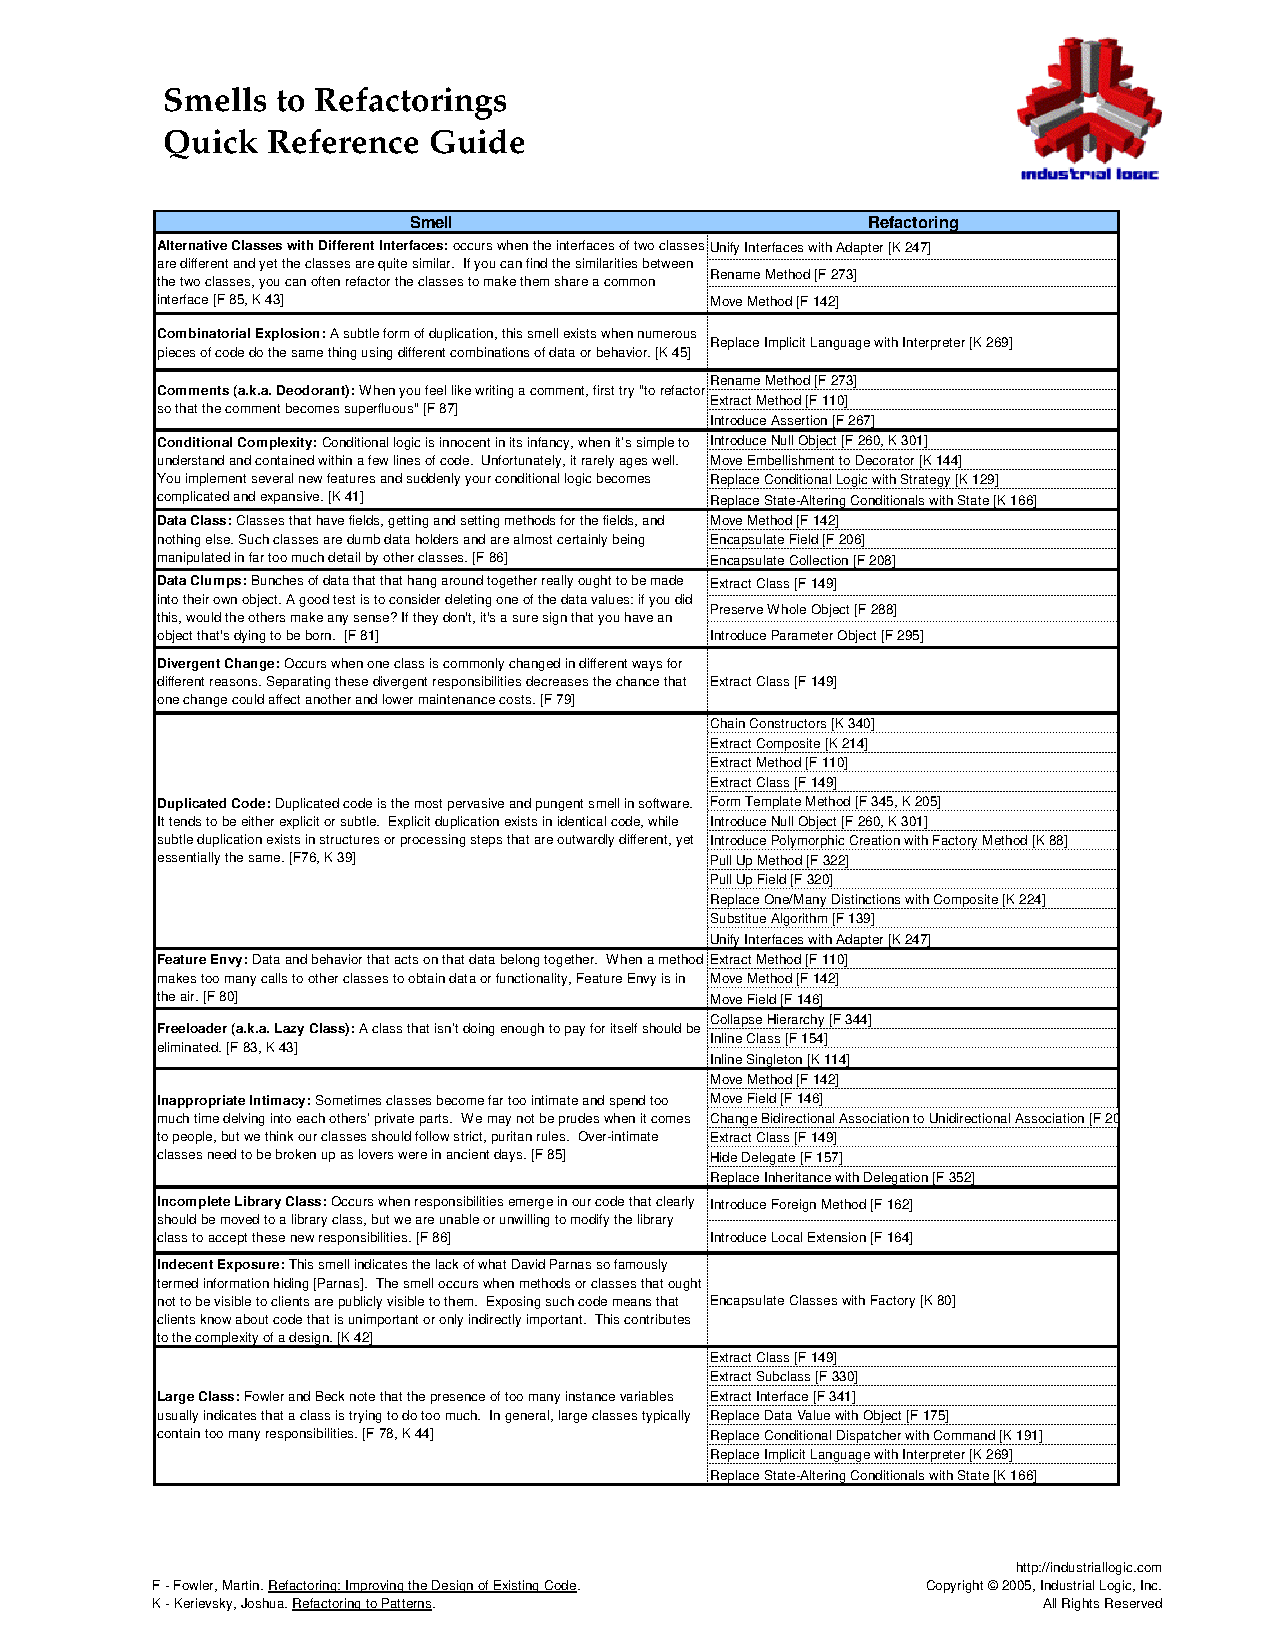
\includepdf[pages={1,2}]{res/smellstorefactorings.pdf}






























\chapter{特别专题:评判可维护性的工具}

\section{评判可理解性的工具}

即使代码格式化得很好,变量和方法的命名也很贴切,但这并不能有效地帮助理解一个拥有上百万行(或者甚至上万行)的程序。为了更好地理解庞大的代码,一个通用的方法是创建工具,这些工具可以提供关注代码“重要”方面的视图。这意味着通过某种方式过滤或聚焦于代码的关键部分,而不是尝试一次性理解整个代码。

\subsubsection{具体方法}
\begin{itemize}
	\item 程序分析工具 (Program Analysis Tools): 这些工具可以自动分析代码,找出其中的模式、依赖关系和可能的问题点。例如,静态代码分析工具可以检测潜在的错误、安全性问题或不良的编码实践。
	\item 软件可视化工具 (Software Visualisation Tools): 这些工具将代码或其结构转化为图形或图像,以便于人类理解。例如,依赖关系图可以显示不同模块之间的依赖,而流程图可以显示程序的执行流程。
	\item 编程语言 (Programming Languages): 选择正确的编程语言或者利用语言的特定功能也可以帮助更好地理解程序。某些编程语言可能通过其设计或特性,如强类型、函数式编程或面向对象的特性,来促进更清晰、更模块化的代码。
\end{itemize}


\subsubsection{程序分析的重要性}
工具需要分析代码以确定感兴趣的属性。这种分析可以揭示代码的各种特征,从而帮助开发者更好地理解和优化代码。

\subsubsection{代码分析的步骤}
\begin{itemize}
	\item 解析代码: 工具首先需要读取并解析代码。
	\item 创建内部表示: 通常,工具会创建一个代码的内部表示,称为"抽象语法树"(AST)。
	\item 查找特征: 内部表示然后被检查,以找到感兴趣的特征。
\end{itemize}


\subsubsection{软件指标}
程序分析工具通常提供来自"软件指标"的测量,这些测量可以帮助评估代码的质量、效率和其他关键特性。

\subsubsection{实例分析}
以下是一些可能的研究或分析主题,其中包括了如何检测代码中的不良现象、开发者在命名、编码和决策中的实践等。
\begin{itemize}
	\item 代码的“坏味道”: 如何检测代码中可能存在的设计或实现问题。
	\item 命名规范的忽视: 开发者有多频繁地忽略了命名标识符的指南。
	\item 非有意义的命名: 开发者使用不具有明确意义的命名的频率。
	\item 函数/方法的参数数量: 开发者在他们创建的函数/方法中有多少参数。
	\item 记录不良决策: 开发者有多频繁地在代码中记录他们所做的不良决策(被称为"自承认的技术债务")。
	\item 代码量的测量: “代码行数”是否提供与“方法数量”或“字段数量”不同的信息。
	\item 关注点的分离度量: 如何确定代码中"关注点分离"的程度。
\end{itemize}



\section{可视化工具}
软件可视化是软件工程领域中的一个大研究领域。例如,IEEE的VISSOFT工作会议专门研究软件可视化,这显示了这一主题的重要性和相关性。一幅画胜过千言万语" — 这句话表达了软件可视化的核心思想,即使用图片来有效地展示软件中的感兴趣方面。通过图像,我们可以更直观、更快速地理解复杂的概念或数据。

软件可视化强调了多个领域的结合,包括排版、平面设计、动画、电影摄影,以及现代的人机交互和计算机图形技术。这些结合在一起,目的是促进人们对计算机软件的理解和有效使用。













\part{程序的可测试性}

\chapter{Improving Testability}

回顾之前的内容,为了测试某个东西,我们需要能够按照我们希望的方式操作它,以便我们可以观察不同输入的后果。换句话说,我们应该有能力控制输入和条件,从而观察其在各种情况下的表现,这是可控性 (Controllability)。为了测试某个东西,我们需要能够看到它实际上在做什么。这意味着我们应该能够观察并测量系统的输出或行为,以判断其是否按预期运行,这叫可观察性 (Observability)。

为了提高一个系统或应用的测试性,需要增强其可控性和可观察性。这是因为:
良好的可控性允许我们模拟各种情况,以验证系统在各种条件下的表现。
良好的可观察性允许我们清晰地看到系统的反应和输出,从而确定它是否满足了预期的需求和标准。

\subsubsection{测试用例的执行流程}

\textbf{IUT的准备:}首先,我们需要为待测单元 (IUT - Implementation Under Test) 设置一个预测试状态。这意味着我们需要确保待测单元在测试之前处于正确且预期的状态,以便我们可以在这个状态下进行测试。

\textbf{提供输入:}在IUT准备好后,我们需要提供特定的输入数据。这些输入是为了触发IUT的某些功能或行为。

\textbf{执行IUT:}带有所给输入的IUT现在可以执行。这意味着我们正在实际运行软件或功能,以观察它如何响应所提供的输入。

\textbf{比较实际与预期的行为:}最后,我们需要比较IUT的实际行为与预期行为。这涉及检查输出或系统行为,以确定软件是否按照预期运行。如果实际行为与预期行为一致,那么测试用例可能会被标记为通过;否则,它会被标记为失败。

\section{使用DIP提升可测试性}

为了提高测试性,我们需要增强观察性(observability)和控制性(controllability)。这两个属性是评估软件的测试性时的关键指标。观察性涉及到我们如何检查和理解软件的内部状态,而控制性涉及我们如何操纵这个状态。
尽管需要观察和控制,但我们仍希望避免破坏封装性,因为封装是面向对象设计的核心原则。如果真的需要破坏封装,我们应该尽量减少其影响。


状态越具体,控制就越困难。这意味着如果我们的软件状态非常具体或详细,那么操纵或更改这个状态就会更加困难。因此,如何使状态变得不那么具体或详细是一个挑战。

DIP是面向对象设计的一种原则,它鼓励软件组件依赖于抽象而不是具体实现。这样,高级模块不会直接依赖于低级模块,而是依赖于它们共同的抽象。
依赖注入是DIP的一种实现方式。通过依赖注入,我们可以控制一个对象的依赖是什么,这样就可以更容易地操纵和观察这个对象的状态。例如,可以注入模拟对象或存根以模拟外部系统或服务,从而提高测试性。

在实际操作中,我们可以利用Mocking技术。具体来说,就是把一个不知道其下一个状态的对象(如Random)继承,重写其不确定的方法,使其确定,从而提升可控制性。

\begin{lstlisting}[language=Java, caption=Mocking Example, label=lst:mocking_ex]
// Not the real ChaoticRandomGen but a mockup of one
public class MockChaoticRandomGen extends Random {
    private double _result;
    private int _count;

    public MockChaoticRandomGen(double r) {
        _result = r;
    }

    public double nextDouble() {
        _count++;
        return _result;
    }

    public void assertTimesCalled(int expected) {
        assertEquals(expected, _count);
    }
}

public class TestSimulation extends TestCase {
    public void testChaotic() {
        Simulation sim = new Simulation();
        
        // Specify the random distribution for test
        Random distribution = new MockChaoticRandomGen();
        
        sim.setRandom(distribution);  // Injection site
        sim.shopperArrives();
        
        // Now guaranteed that new shopper is chaotic
        distribution.assertTimesCalled(1);  // observe
        
        // other parts of test
    }
}
	
\end{lstlisting}

一旦我们开始创建 "模拟 "类,我们不妨通过添加更多支持测试过程的职责,使它们尽可能有用。
增加更多支持测试过程的职责,包括提供观察所发生情况的方法。

一些成熟的Mock变种供我们使用:

\subsubsection{Stubs}
Stubs 是最基础的模拟类型,它们提供完全简单的实现,并作为占位符存在,以便代码能够编译并创建实例。Stubs 在集成测试中经常被提及。在集成测试中,当开发者想要测试某个组件与其他组件的交互,但这些组件尚未实现或可用时,他们可能会使用 stub。但是使用 Stubs 的通常形式可能需要更改正在测试的代码,这可能会导致代码的紧耦合。

\subsubsection{Fakes}
Fakes 是非常简单的 mocks。它们提供功能更为完整的实现,但通常会避免使用真实的资源,如数据库或网络服务。Fakes 是非常简单的 mocks。它们提供功能更为完整的实现,但通常会避免使用真实的资源,如数据库或网络服务。

\subsubsection{Mocks}
Mocks 不仅提供受控的行为,还可以观察它们是如何被使用的。这意味着,除了模拟某个行为之外,Mocks 还可以验证他们是否按预期被调用。jmock, easymock, 和 mockito 是流行的 Java 模拟库,可以帮助开发者创建和管理 mock 对象。

\subsubsection{GoogleMock}
oogleMock是一个流行的模拟框架,它是 googletest 的一部分。googletest 是 Google 提供的一个开源的 C++ 测试框架。使用 GoogleMock,C++ 开发者可以轻松地为他们的代码创建 mock 对象。

\section{总结}
\textbf{设计选择会影响可测试性---特别是 DIP(依赖注入)的使用通常会提高可测试性(但也有其他原因)。}

在软件开发中,模拟和模拟的变种(如 Stubs、Fakes 和 Mocks)为开发者提供了强大的工具,以在没有真实组件或服务的情况下测试代码。这些模拟方法可以提高测试的速度和灵活性,并帮助确保代码的质量和健壮性。

\chapter{Test Driven Development}

创建软件涉及到许多决策,这些决策可能关乎软件架构、设计模式、算法选择、数据结构、代码风格等。理想情况下,开发者总是希望做出正确的决策,以确保软件的高质量和长期的可维护性。启发式可以为开发者在面临决策时提供指导。例如,设计原则、最佳实践或其他经验法则。
然而,即使有了这样的指导,仍然存在一些决策难以作出,因为它们可能涉及到多个交叉关注点或因项目特定的约束而变得复杂。

鉴于上述的挑战,需要一个通常(或至少经常)有助于做出良好决策的过程。

\section{测试驱动开发}

TDD是一个软件开发过程,其中开发者首先为一个新的功能或修复写下一个失败的测试,然后写代码使测试通过,最后重构代码以达到所需的标准。在TDD中,开发是由已经写好的测试指导的。这意味着在实际编写功能代码之前,开发者已经明确了期望的行为和输出。为了让测试能够执行,设计必须支持测试。这意味着,代码结构、模块划分和依赖关系等都需要被设计成易于测试的。

\subsubsection{具体步骤}

\begin{itemize}
	\item \textbf{添加一个小测试:}选择一个能够让现有实现失败的测试。
	\item \textbf{运行所有测试:}确保新添加的测试失败。
	\item \textbf{做一个小改动:}只修改足够使新的测试通过的代码,这一阶段不需要考虑代码的优雅性或最佳实践。
	\item \textbf{运行测试并成功:}确保所有测试(包括新添加的)都通过。
	\item \textbf{重构以消除重复:}在确保所有测试通过后,进行代码重构,以消除代码中的重复部分或提高代码质量。
\end{itemize}

\subsubsection{Martin的三个法则}

\begin{itemize}
	\item \textbf{不得编写生产代码,直到您编写了一个失败的单元测试:}这确保了对功能的期望在功能代码之前得到明确。
	\item \textbf{您不得编写超过足够导致失败的单元测试,且不编译也算作失败:}这避免了过度测试,鼓励开发者首先关注主要的失败点。
	\item \textbf{您不得编写超过足够通过当前失败测试的生产代码:}这强调了小步快跑,确保每一步都有明确的目标。
\end{itemize}

需要保持代码整洁,包括测试代码。代码的整洁性不仅使其易于阅读和维护,还可以避免将来的错误和复杂性。

\paragraph{测试驱动开发 (TDD) 并不是关于如何创建好的测试}
TDD的核心是关于如何设计和实现代码,而不仅仅是关于测试。虽然测试是TDD的关键组成部分,但TDD的真正价值在于它对软件开发生命周期的影响,以及它如何帮助开发者编写更好、更可维护的代码。

\paragraph{所有关于可维护代码的规则都适用于测试代码}
测试代码就像生产代码一样重要,它需要同样的注意力和照顾。考虑以下两个关键点:

\begin{itemize}
	\item \textbf{可理解性:}这是关于测试的明确性和目的。当其他开发者(或者您自己在未来)查看测试时,他们应该能够轻松地理解测试的目的,它测试了哪些功能,以及哪些测试与特定的代码段有关。

	\item \textbf{可变性:}当生产代码发生变化时,相关的测试可能也需要调整。开发者应该能够轻松识别哪些测试与特定代码段有关,以便在代码更改后更新或修改这些测试。
\end{itemize}

\paragraph{TDD不提供设计}尽管TDD鼓励良好的编程实践和重构,但它本身并不直接提供软件的设计或架构。设计和架构的质量依赖于开发者的经验和知识。

\paragraph{TDD $\neq$测试}TDD并不等于全面的测试。尽管TDD侧重于编写测试并确保代码按照测试的期望来实现,但进行适当的测试需要更多的测试用例。测试应当在API的级别。

我们并不总是明显的知道接下来应该写什么样的测试。在某些情况下,为了确定一个小的失败测试,可能需要添加已经通过的测试。如何进行最简单的更改以使测试通过并不总是明确的。这里的“最简单”可能会根据开发者的经验而有所变化。

识别存在哪些重复可能是困难的。那么,什么构成了“重复”呢?
“重复”包括“冗余/不必要的”和“数据重复”。
这似乎是进行“好的工程实践”的地方。
如何去除这种重复可能是困难的。
如果处理得不对,其后果是不明确的。但是,“回退”被视为一个可行的选项。

\paragraph{TDD是否排除了某些(好的)设计?}
例如,使用TDD可以得到雨量的过滤然后处理的设计吗?(循环是重复的吗?)

\section{相关研究}

一项研究涉及学生和工业团队,两者都有不同的控制水平。

TDD团队的特点:
更小的类和方法:与非TDD团队相比,使用TDD的团队倾向于编写更小的类和方法。这可能是因为TDD鼓励开发者频繁地进行小规模的迭代和改进。
更低的``复杂性":TDD团队的软件复杂性较低。这可能意味着他们的代码更简洁、更容易理解和维护。
更低的``耦合" (CBO):TDD团队的代码在CBO(类之间的耦合度)上得分较低。低耦合意味着各个组件或类之间的依赖关系更少,这可以增强软件的可维护性和灵活性。
``内聚" (LCOM5) 没有明显趋势:LCOM5是一个测量类内聚度的指标。在这项研究中,TDD与非TDD团队在内聚度上没有明显差异。

学生团队与工业团队的差异:
学生团队与工业团队之间在上述指标上的差异较大。特别是在工业团队中,使用TDD与否之间的差异较小。这可能是因为工业团队通常拥有更多的经验和培训,他们可能已经采用了其他的最佳实践,从而使TDD的效果相对较弱。

\section{总结}
TDD可带来我原本不会选择的成功设计。关于成本/效益权衡仍存在各种问题,但我更倾向于相信而非不相信。






































\chapter{Examination}
\section{Potential Assessment Questions}
\subsection{3.2}
Martin’s heuristic for good names Use Intention-Revealing Names says that the name should answer the big questions, including “how the variable, function, or class is used.”
Explain how answering this question improves comprehensibility in terms of the program comprehension model.

The program comprehension model essentially deals with how programmers understand existing code – be it written by someone else or even by the same developer but some time ago. Understanding how code works is essential for debugging, enhancing, or reusing it. The model implies a cognitive process, where a developer constructs a mental model (or representation) of the code by combining the explicit information given in the code with their prior knowledge (often termed as Knowledge Base or KB).

Let's analyze Martin's heuristic for good names, particularly "Use Intention-Revealing Names", in the context of the program comprehension model:

Explicit Information: When names are intention-revealing, they serve as explicit information about what that piece of code (variable, function, or class) is supposed to do. A good, descriptive name reduces the ambiguity or uncertainty about its purpose.

Reduced Dependency on External Resources (ER): If a name doesn't convey its intention, developers might need to consult external resources like documentation, or other parts of the code to understand its purpose. In the comprehension model, accessing ER is less efficient than accessing the Knowledge Base (KB) or Mental Model (MM). Intention-revealing names reduce the need to access ER.

Efficient Interaction with Knowledge Base (KB): Developers come with a set of prior knowledge about naming conventions, design patterns, programming paradigms, etc. When they encounter an intention-revealing name, it resonates with their existing knowledge, making the comprehension process smoother and quicker.

Building an Accurate Mental Model (MM): For effective debugging and modification, developers should build a correct and comprehensive mental model of the code. Descriptive names aid in constructing this model by providing clear and unambiguous cues about how each component fits into the broader picture.

Reduced Cognitive Load: The human working memory, often likened to the MM, has a limited capacity. If developers spend significant mental resources trying to decipher the purpose of poorly named variables or functions, it detracts from their ability to understand the broader logic or flow of the program. Intention-revealing names streamline the comprehension process by reducing this cognitive overhead.

In conclusion, using intention-revealing names is a heuristic that aligns well with the program comprehension model. By providing clear, unambiguous cues about the purpose and usage of code components, these names facilitate a more efficient and accurate understanding of the code, leading to better maintainability and fewer errors.

马丁的 "好名字启发式"(heuristic for good names Use Intention-Revealing Names)认为,名字应能回答重大问题,包括 "变量、函数或类是如何使用的"。
从程序理解模型的角度解释回答这个问题如何提高可理解性。

程序理解模型主要涉及程序员如何理解现有代码--无论是别人编写的代码,还是同一开发人员在很久以前编写的代码。理解代码的工作原理对于调试、增强或重用代码至关重要。该模型意味着一个认知过程,开发人员通过将代码中提供的显式信息与其先前的知识(通常称为知识库或 KB)相结合,构建代码的心智模型(或表征)。

让我们在程序理解模型的背景下分析一下马丁关于好名字的启发式,尤其是 "使用能反映意图的名字":

显式信息: 当名称能够揭示意图时,它们就成为了一段代码(变量、函数或类)应该做什么的明确信息。一个好的、具有描述性的名称可以减少其目的的模糊性或不确定性。

减少对外部资源(ER)的依赖: 如果名称不能表达其意图,开发人员可能需要查阅文档等外部资源或代码的其他部分,才能理解其目的。在理解模型中,访问 ER 的效率低于访问知识库(KB)或心智模型(MM)。揭示意图的名称可减少访问 ER 的需要。

与知识库(KB)的高效交互: 开发人员拥有一套关于命名约定、设计模式、编程范例等方面的先验知识。当他们遇到揭示意图的名称时,就会与现有知识产生共鸣,从而使理解过程更加顺畅和快速。

建立准确的心理模型(MM): 为了进行有效的调试和修改,开发人员应为代码建立一个正确而全面的心智模型。描述性名称可提供清晰明确的提示,说明每个组件是如何融入大局的,从而有助于构建这一模型。

减少认知负荷:人类的工作记忆通常被比作 MM,其容量是有限的。如果开发人员花费大量的脑力去解读命名不清的变量或函数的目的,就会影响他们理解更广泛的程序逻辑或流程的能力。揭示意图的名称可以减少这种认知开销,从而简化理解过程。

总之,使用揭示意图的名称是一种启发式方法,与程序理解模型十分吻合。通过对代码组件的目的和用法提供清晰明确的提示,这些名称有助于更有效、更准确地理解代码,从而提高可维护性,减少错误。

\subsection{4.1}
Explain, in terms of the program comprehension model, why we would generally expect names created by joining whole words together would lead to more comprehensible code than if we used names that are formed by taking the first letters of the same words (acronyms).

The program comprehension model describes the cognitive process developers undergo when trying to understand a piece of code. This involves creating a mental model (MM) based on the code itself and their prior knowledge (Knowledge Base, or KB). When they can't figure something out based on these two sources, they often resort to External Resources (ER) such as documentation or other reference materials.

Explicitness and Ambiguity: Names created by joining whole words are more explicit and convey more information than acronyms, which are often ambiguous. For a developer reading the code, whole words are easier to understand without referring back to prior context or definitions, thereby reducing cognitive load.

Knowledge Base (KB) Access: Whole words often resonate better with a developer's existing knowledge. Acronyms might not immediately connect with the KB unless the developer is familiar with the specific context where the acronym was created.

Reduced Dependency on External Resources (ER): When encountering an unfamiliar acronym, a developer might need to resort to external documentation or search for the place where the acronym was first defined, leading to inefficiencies. Whole-word names often make the code self-explanatory, reducing the need to refer to ER.

Building an Accurate Mental Model (MM): Whole words contribute to a clearer and more accurate mental model, as they provide more context. Acronyms, being condensed and potentially ambiguous, might lead to misconceptions or gaps in the MM.

从程序理解模型的角度解释,为什么我们通常会认为,与使用由相同单词的首字母组成的名称(缩略语)相比,由整个单词连接而成的名称更容易理解代码。

程序理解模型描述了开发人员在试图理解一段代码时所经历的认知过程。这包括根据代码本身和他们先前的知识(知识库或 KB)创建一个心智模型(MM)。当他们无法根据这两个来源搞清楚某件事情时,他们通常会求助于外部资源(ER),如文档或其他参考资料。

明确性和模糊性: 通过连接整词创建的名称比缩略语更明确,传递的信息也更多,而缩略语往往模棱两可。对于阅读代码的开发人员来说,整词更容易理解,无需参考先前的上下文或定义,从而减轻了认知负担。

知识库(KB)访问: 整词通常能更好地与开发人员的现有知识产生共鸣。缩略词可能无法立即与知识库产生共鸣,除非开发人员熟悉缩略词产生的具体语境。

减少对外部资源(ER)的依赖: 遇到不熟悉的首字母缩略词时,开发人员可能需要借助外部文档或搜索首次定义该首字母缩略词的地方,从而导致效率低下。整词名称通常会使代码变得不言自明,从而减少参考资源的需要。

建立准确的心智模型(MM): 全词提供了更多的上下文,有助于建立更清晰、更准确的心智模型。首字母缩略词过于简洁,可能会产生歧义,从而导致心智模式中出现误解或空白。

\subsection{4.1}
Give an example where using an acronym for a name is likely to produce more comprehensible code than if the full words were used.

Consider a widely recognized and accepted acronym like "HTTP" (Hypertext Transfer Protocol). In the context of web development or networking:

Using HTTPRequest is likely to be more comprehensible than HypertextTransferProtocolRequest because:

Familiarity: For developers in this domain, "HTTP" is a familiar and instantly recognizable acronym.

Brevity: Shorter names are quicker to read and reduce visual clutter in the code, especially when used frequently.

Industry Standard: Since "HTTP" is an industry-standard term, using the full form might even seem unconventional and counterintuitive.

Thus, while whole-word names generally enhance comprehensibility by providing clarity, there are situations where well-established acronyms can be more effective.

请举例说明使用缩写名称可能比使用全称产生更易理解的代码。

考虑一下像 "HTTP"(超文本传输协议)这样被广泛认可和接受的缩写。在网络开发或网络连接中:

使用 HTTPRequest 可能比使用 HypertextTransferProtocolRequest 更容易理解,因为:

熟悉: 对于该领域的开发人员来说,"HTTP "是一个熟悉的缩写,一眼就能辨认出来。

简洁: 较短的名称阅读起来更快,并能减少代码中的视觉干扰,尤其是在频繁使用时。

行业标准: 由于 "HTTP "是一个行业标准术语,使用全称可能会显得不合常规,有违直觉。

因此,虽然全词名称通常能通过提供清晰度来提高可理解性,但在某些情况下,成熟的缩写可能会更有效。

\subsection{4.2}
For the comprehension model discussed in the course, explain the difference between the mental model and the knowledge base. Use (small!) code examples to illustrate the difference.

The comprehension model often referred to when discussing software comprehension, posits that readers of code build an internal representation (or "mental model") of the code, influenced by their prior knowledge and experiences (the "knowledge base"). Let's break down these two concepts:

Mental Model:

The mental model is a cognitive representation of the system or code. When a developer reads code, they form an understanding of what that code does, how it works, and its purpose. This understanding, built progressively, is the mental model.

It's dynamic and evolves as a developer reads more code or gains more context.

The mental model isn't always correct; misconceptions or misunderstandings can be introduced based on how the code is written or the developer's own biases.

Example:

def add(a, b):
return a + b

Upon reading this code, a developer might form the mental model: "This is a function that takes two parameters and returns their sum."

Knowledge Base:
The knowledge base comprises all the prior knowledge, experiences, and concepts that a developer brings to the table when reading code. This includes programming constructs, patterns, algorithms, domain-specific knowledge, and even prior experiences with similar code.

It's static in the sense that, at any given moment, it represents what the developer knows up to that point. However, it's constantly expanding and evolving over time as the developer learns and experiences more.

Example:

def fibonacci(n):
if n <= 1:
return n
else:
return fibonacci(n-1) + fibonacci(n-2)

A developer with prior knowledge about the Fibonacci sequence (from their knowledge base) will immediately recognize this recursive pattern and comprehend the code's intention. In contrast, a developer without that prior knowledge might need more time to build their mental model around how this function works.

针对课程中讨论的理解模型,解释心智模型和知识库之间的区别。使用(小型!)代码示例来说明两者的区别。

在讨论软件理解时经常提到的理解模型认为,代码读者受其先前知识和经验("知识库")的影响,建立了代码的内部表征(或 "心智模型")。让我们来分解这两个概念:

心智模型:

心智模型是对系统或代码的认知表征。当开发人员阅读代码时,他们会对代码的作用、工作方式和目的形成一种理解。这种逐步形成的理解就是心智模型。

它是动态的,随着开发人员阅读更多代码或获得更多上下文而不断发展。

心智模型并不总是正确的;基于代码的编写方式或开发人员自身的偏见,可能会产生误解或误解。

代码略。

在阅读这段代码时,开发人员可能会形成这样的心理模型: "这是一个接收两个参数并返回其和的函数。

知识库:
知识库包括开发人员在阅读代码时所掌握的所有先前知识、经验和概念。其中包括编程结构、模式、算法、特定领域的知识,甚至是以前使用类似代码的经验。

它是静态的,因为在任何给定的时刻,它都代表着开发人员到那时为止所掌握的知识。但是,随着时间的推移,随着开发人员学习和体验的增加,它也在不断扩展和发展。

代码略。

如果开发人员事先了解斐波那契数列的相关知识(来自他们的知识库),就会立即识别出这种递归模式,并理解代码的意图。相比之下,不具备相关知识的开发人员可能需要更多时间来围绕该函数的工作原理建立心智模型。

\subsection{5.1}
Consider the following code fragment (which comes from the JUnit 4.11 implementation for org.junit.Assert):

/**
* Protect constructor since it is a static only class
*/
protected Assert() {
    }

Briefly comment on the usefulness of this comment.

This is a constructor for the Assert class, which is declared as protected. this constructor is empty and does not perform any operations.

The comment that says "Protect constructor since it is a static only class" is meant to protect the constructor since it belongs to a class that has only static methods.

Now, let's relate this code to the Program Comprehension Model (PCM):

MM (Mental Model): The code reader needs to form a mental model of the code to understand how it works. Without annotations, the reader may have questions about why the constructor is empty, why it is protected, and so on.

KB (Knowledge Base): The reader's prior knowledge may tell them that when a class has only static methods, it is often prevented from instantiating it. But this is not known to everyone, especially developers who are not familiar with Java or OOP.

ER (External Representation): The code and comments themselves constitute the external representation. The comments provide additional context here, explaining why the constructor is protected.

Assimilation Process: This is the process of merging ER into MM and KB. Annotation helps this process as it provides the reader with the reason why the constructor is protected.
Effectiveness and Efficiency.

Effect: With this comment, the reader of the code can more quickly understand why the constructor is empty and why it is protected. This makes the code more self explanatory.
Efficiency: Without the annotation, readers may need more time and effort to surmise why the constructor is protected. But with this comment, they can get the answer immediately, improving the efficiency of understanding the code.

请看下面的代码片段(来自 JUnit 4.11 的 org.junit.Assert 实现):

代码略

请简要说明该注释的用处。

这是一个Assert类的构造函数,它被声明为protected。此构造函数是空的,不执行任何操作。

注释指出:“Protect constructor since it is a static only class”,意思是为了保护该构造函数,因为它属于一个只有静态方法的类。

现在,我们将这段代码与程序理解模型(Program Comprehension Model)进行关联:

MM (Mental Model): 代码阅读者需要形成一个关于代码的精神模型,理解它是怎样工作的。没有注释,阅读者可能会对为什么构造函数是空的、为什么它是受保护的等有疑问。
KB (Knowledge Base): 阅读者的先前知识可能告诉他们,当类只有静态方法时,常常会阻止实例化它。但这并不是所有人都知道的,特别是那些不太熟悉Java或OOP的开发者。
ER (External Representation): 代码和注释本身构成了外部表示。注释在这里提供了额外的上下文,解释了为什么构造函数是受保护的。
Assimilation Process: 这是将ER合并到MM和KB中的过程。注释帮助了这一过程,因为它为阅读者提供了为什么构造函数受保护的原因。
效果与效率:

效果:有了这个注释,代码的阅读者可以更快地理解为什么构造函数是空的和为什么它是受保护的。这使得代码更具有自解释性。
效率:在没有注释的情况下,阅读者可能需要更多的时间和努力来推测为什么构造函数是受保护的。但有了这个注释,他们可以立即得到答案,提高了理解代码的效率。

\subsection{6.1}
Suppose you were shown two designs for a system, Design A, which has 5 classes, and Design B, which has 9 classes. For both designs, you agree that the classes are reasonable. Which design do you think is likely to be more comprehensible and why?

Number of Classes: Although Design B has more classes, it may be easier to understand if these classes make the responsibilities of each class clearer and reduce the complexity between classes. In contrast, Design A may have only five classes, but if the interactions between them are very complex, it may be difficult to understand.

Effectiveness: If each class in Design B has a clear, single responsibility and clear interactions with other classes, it may be easier for developers to form an accurate mental model, even if there are more classes.

Efficiency: If the five classes in Design A are relatively functionally focused, it may take more time and effort to understand the internal details of each class. In Design B, on the other hand, each class may be smaller and more focussed, making understanding each class a quicker and more straightforward task.

Conclusion: It is not possible to conclude which design is easier to understand from the number of classes alone. Actual understandability depends on the clarity of the classes, the interactions between them, and how well they match the developer's existing knowledge. In order to truly assess which design is easier to understand, an in-depth look at the specific implementation and structure of each design is required.

假设有人向你展示了一个系统的两个设计方案,设计 A 有 5 个类别,设计 B 有 9 个类别。对于这两种设计,你都认为类是合理的。你认为哪种设计更容易理解,为什么?

类的数量: 虽然设计 B 有更多的类,但如果这些类能使每个类的职责更清晰,并减少类之间的复杂性,那么设计 B 可能更容易理解。相比之下,设计 A 可能只有五个类,但如果它们之间的交互非常复杂,则可能难以理解。

有效性: 如果 "设计 B "中的每个类都有明确、单一的职责,并且与其他类的交互关系也很清晰,那么即使类再多,开发人员也更容易形成准确的心智模型。

效率: 如果 "设计 A "中的五个类功能相对集中,那么开发人员可能需要花费更多时间和精力来了解每个类的内部细节。而在设计 B 中,每个类可能更小、更集中,因此理解每个类是一项更快、更直接的任务。

结论 不能仅从类的数量来断定哪种设计更容易理解。实际的可理解性取决于类的清晰度、类之间的交互以及它们与开发人员现有知识的匹配程度。为了真正评估哪种设计更容易理解,需要深入研究每种设计的具体实现和结构。

可选回答1:

设计b具有更多数量的类,所以每个类更小
如果类更小,更可能匹配单一概念。如果一个类更能匹配在上下文模式或设计模式的单一概念,它越可理解。
如果类更小,他更可能只有一个职责和更具有凝聚力,所以可以花费更少的时间来阅读和理解类,这提高了效率,所以具有更高可理解性。

可选回答2:

B更容易理解:
1. 单一职责原则:划分更多的类意味着每个类具有更少的功能。在尝试理解程序时,可以减少每个类经由内化过程到Mind Model的时间。
2. 内聚性:A中的类之间可能有复杂的交互,B的类之间的关系可能相对简单。这同样使得内化过程大幅减少。
3. 抽象:更多的类可能意味着更高的抽象程度。这意味着在尝试理解程序时,无需理解一些类中的具体代码,可以从Knowledge Base中推测类的作用。
\section{Analysing Methods}

Comprehensibility - PCM.

Alterability - Change cases.

Testability - Controllability and Observability.
\section{2022 Test 1 Notes}

对于每道题,请先写一遍题目中提到的定义。

\subsection{Q2}
\subsubsection{a}
软件维护的种类:corrective, adaptive, preventative, perfective。
增加一个特性是perfective。
\subsubsection{b 讨论可变性:}
可更改性是指如何在不引入缺陷或降低现有产品质量的前提下,有效且充分地更改产品系统。
4.3 中有很多地方需要修改,而 5.1 中的修改只有第 14、61、62 和 64 行(后三行都在一个方法 changePlayer() 中)。因此,仅仅修改 4.3 就需要更多的工作(\textbf{效率更低})。

由于要修改的地方较多,而每个地方都有可能出错(例如漏掉),因此要修改的地方越多,出错的可能性就越大(假设出错的可能性差不多--在本例中是一样的,因为在两种实现中要做的修改是一样的)。由于 4.3 需要改动的地方较多,在改动时出错的几率也较高,因此\textbf{有效性}较低。

提示:可变性与可理解性互相独立。本题中请不要讨论可理解性。

\subsection{Q3 类的大小/数量如何影响测试性}
比较:

小的类会比大的多(因为功能是一样的)。假设每个类都能提供相同水平的可观察性和可控制性,这意味着小的将比大的拥有更多的可观察性和可控制性,因此更容易测试。

事实上,小类可能比大类更具可观察性和可控性。类越大,需要为测试正确设置的状态就越多(Controllability),需要查看(Observability)的东西就越多,以便在测试后确认类中的对象是正确的。也就是说,需要花费更多精力来进行测试,这就不如小类的效率(Efficiency)高。

有单一责任(SRP)的类通常比没有单一责任的类小。

当一个类依赖于另一个类时(例如,通过调用另一个类中对象的方法),测试该类就需要额外的工作来设置另一个类中的对象。小类更有可能不依赖于其他类,因此所需的工作量会更少(Efficiency)。

\subsection{Q4 PCM}
\subsubsection{解释KB中的知识的特性}

这种知识优势必须存在(在知识库中),以便能够理解任何代码,但这种知识并不具体涉及所理解的代码。

String result = obj.someMethod(); 例如,对于这段代码:我们将使用 Java 语法知识来认识到 someMethod() 必须返回字符串(假设代码能编译)。知识库中的这些知识类似于 "当赋值运算符 (=) 右侧有一个方法调用,左侧有一个 java.lang.String 类型的变量时,该方法必须返回一个 String 值"。这不是专门关于代码的知识,因此不会出现在 MM 中。
MM 中的知识应该是这样的:"变量 obj 来自 A 类,A 类中的方法 someMethod() 返回一个描述对象当前状态的字符串"。

\subsubsection{解释陌生代码如何内化}
这段代码位于 ER 中。理解这段代码需要 Java 方面的知识,尤其是 = 左边和右边的含义。此外,还需要了解方法调用语法和方法调用的含义。这些知识与代码本身无关(见第(a)部分),因此必须放在知识库中。
如果您没有相关的 Java 知识,也就是说知识库中没有这些知识,那么您就需要获取这些知识。这就需要查阅有关 Java 的描述,这些描述可以在 ER 中找到。一旦掌握了这些知识,它们就会出现在知识库中。
一旦掌握了必要的 Java 知识,您就可以通过 AP 来解释代码(在 ER 中),从而确定代码的作用,并根据这些新信息更新 MM。

请注意,需要引用模型中的每一个组件。

\subsection{Q5 可读性}

\subsubsection{a 可读性如何影响可理解性}
识别元素(如循环体)或区分元素(如一个变量与另一个变量)或确定哪些元素属于同一个元素越困难,阅读就越困难。 如果阅读困难,那么理解的效果和/或效率就会降低。因此,可读性低就意味着可理解性低。

\subsubsection{b 巨量代码空白如何影响可理解性}
卫生间管道提示建议不要让多个函数的代码同时出现在屏幕上。每行之间有多个空行可能会降低可理解性,因为读者需要上下滚动屏幕来阅读和理解一个功能。如果阅读一个功能需要时间,那么从 ER 到 KB/MM 的内化过程就会延长。从而影响理解一个功能的效果和效率。


\subsection{Q6 四连棋游戏}

\subsubsection{a 棋子类是否必要}

为玩家投放到网格中的物品(从现在起将称为 "令牌")引入一个类别会增加理解该类别所需的额外工作。

不过,我们可以考虑另一种方法。必须要有一些代码来显示网格中是否有标记物。这些代码至少需要记录它属于哪个玩家,可能还需要记录它的颜色。每次有人查看这段代码时,他们都必须记住这段代码在做什么。

可维护性的定义(及其所有方面)适用于整个生命周期内的整个实现。因此,虽然在第一次查看类的代码时需要付出额外的努力,但预计在大多数情况下,这些代码都不会再被查看。从长远来看,该类的成本可能与查看备用代码并记住其含义的成本相差不大。

此外,如果需要对令牌进行任何更改(可更改性),如果有一个类,那么所需的努力将仅限于更改该类。如果只有一些代码,那么该代码存在的每个地方(例如,检查行中哪个位置未填写的代码、检查是否有中奖行的代码)都必须更改。这种工作量(效率)可能远远超过仅仅更改类的工作量。

我们需要的主要方法是一个能确定由哪位玩家出牌的方法(例如类似 getColour()的方法)。在真实游戏(上下文模式)中,没有什么能阻止玩家交换他们使用的颜色)。

\subsubsection{b “棋子”还是“令牌” - PCM}
一个类与上下文或设计模式中所代表的概念越一致,就越容易理解。鉴于问题中对游戏的描述总是提到 "令牌",这似乎比任何其他选择(包括 "棋子")都更好。

\textbf{The more a class is consistent with the concept it represents from the context or design schema, the more comprehensible it will be.}

\subsubsection{c 什么是正确的对象数量}

在现实世界的游戏中,必须至少有 42 个代币(网格中最多有 42 个地方可以放置代币)。据推测,游戏在出售时还会附带一些备用代币,以防代币丢失。无论总共有多少代币,它们在游戏开始时都是存在的。
在软件中,我们不必担心代币丢失的问题(假设),因此这表明至少应该创建 42 个代币,以获得与上下文模式的最佳匹配。
但在软件中,我们不需要一开始就准备好所有计划使用的东西,因为我们可以根据需要创建它们(假设)。在本例中,将为所示示例创建 14 个标记。

\subsubsection{d 再确定2个实体类}

例如:Grid、Player、Connect4、Column(或类似名称): 网格、玩家、Connect4、列(或类似名称)。位置(或类似名称)可能是不需要的(与 "Noughts and Crosses "游戏不同,玩家并不选择网格中的特定位置,而只是选择列),但允许使用。
与 Noughts and Cross 不同,玩家不会选择网格中的特定位置,只会选择列),但可以使用。
对于这种情境模式来说,"棋盘"(Board)不是一个好名字,因为在描述中使用了 "网格 "一词(而且使用的也不是通常意义上的 "棋盘")。


\subsection{Q7 封装如何支持可维护性}
封装用于支持类所代表的抽象,尤其是如何管理内部状态。如果一个类的设计允许内部状态以与抽象不一致的方式发生变化,则表明封装存在问题。

如图所示的类是用来表示玩家在 "十进制 "游戏中选择的移动位置。一旦玩家做出了选择,就不能更改(上下文模式)。设置器方法(setRow() 和 setCol())的存在使得坐标对象所代表的位置可以更改。这与上下文模式的预期不一致,因此 "破坏了封装"。

类中的每个方法都会为理解它带来代价。如果这种代价是不必要的,就像 "坐标 "类中的 setter 方法一样,那么就会降低理解它的效率(Efficiency),从而降低可理解性。可理解性是可维护性的一个方面,因此这意味着可维护性会降低。

如果使用 setter 方法,就有可能错误地改变坐标对象的状态,从而产生故障(Effectiveness)。

注意,虽然获取器对于 "坐标 "所代表的抽象来说并不是必需的,但它们并不会改变对象的状态,因此问题不大(仍有可比性代价)。然而,它们的存在确实为类提供了可观察性,这将有助于可测试性,因此在这种情况下需要权衡利弊。请注意,构造函数支持可控性,因此不需要设置器来实现可控性。

\subsection{Q8 减少缩进层级对可理解性的影响}

可理解性是指理解代码过程的效率和效果。然而,评估可理解性不应局限于一次性查看代码。它必须在代码的整个生命周期中进行评估。

就问题中的两个版本而言,虽然重构后的版本确实 "有更多的代码",但要正确评估可理解性,就必须考虑这些额外代码在整个生命周期中的影响。如果每次查看 checkDraw() 方法时都要查看额外的代码,那么就会增加成本,因此重构版本的效率较低,可理解性也较低。

但是,通过选择新方法的名称(isRowFull),我们希望在第一次读取该方法后,在查看 checkDraw() 方法时再也不用查看它。然而,在原始代码中,"如果 (\_grid[row][col] == ''),代码是怎么回事?"每次都会被问到,而且回答这个问题要比查看 isRowFull() 方法的调用花费更多精力。因此,总体而言,重构代码将降低成本,从而提高可理解性。

\section{2022 Test 2 Notes}

\subsection{Q1 Design Patterns}

\subsubsection{a 请解释备忘录模式,包括主要成分,关系}

有三个要素: Memento, Originator, and Caretaker。Memento对象由Originator创建。它代表了Originator在某一特定时间的足够状态(快照),通过使用 Memento 中的内容,始发者可以恢复到完全相同的状态。记忆体存储在Caretaker中。Caretaker 绝不能访问 Memento 的内部状态,因为这会破坏封装。当Originator的状态需要恢复时,Caretaker会将之前创建的Memento交给它,然后Originator就可以使用Memento恢复自己的状态。

因此,关键的关系是,Memento 由Originator创建,并存储在Caretaker中。

\subsubsection{b}

\paragraph{复合模式如何影响可理解性}
复合是一个不容易理解的概念。在实现过程中,如果有人不知道如何使用 Composite,那么他很可能需要花费很多精力才能理解,也就是说,可理解性将会降低。
另一方面,如果有人知道复合设计模式,即知识库中有这种设计模式,那么理解它的使用就不那么困难了。

因此,关键的假设是知识库中的内容。

\paragraph{复合模式如何影响可变性}
新叶子的添加不会影响使用复合元素的其他元素,也就是说,不会改变组件和复合元素。因此,如果唯一的改动是在组合元素中添加一些内容(如问题 3 (d)),那么大部分的实现都不需要改动。这就减少了工作量,降低了犯错误的机会(有效性),从而提高了可变更性。如果更改的范围比叶子更广(例如,需要更改组件接口),则需要更多的工作(但无论是否使用 Composite,都可能需要更多的工作)。

因此,关键的假设是变化是什么。

\subsubsection{c 设计模式一般会如何影响可维护性}

可理解性。大多数设计模式都很复杂,不易理解。如果所使用的 DP 不在知识库中,那么实现时就需要花费更多精力(即效率)来理解,从而降低了可理解性。反之,如果所使用的 DP 在知识库中,那么理解这些复杂代码的工作量就会减少,从而提高可理解性。

可变更性。许多 DP 都支持更改。例如,Composite 允许添加叶子;Observer 允许添加新的观察者,而无需对主体或其他观察者进行任何更改。

可测试性。鉴于 DP 中各元素之间复杂的互动关系,测试的设置可能会很复杂。

\subsection{Q2 Temporary Field}

\subsubsection{a 临时字段如何影响可理解性}

关键在于所涉及的字段是不必要的。可以通过引入一个参数来删除它。在试图理解一个方法的实现时,查找参数的定义比查找字段的定义花费的时间要少,因此理解一个带参数的方法(即更高效)要比理解一个使用字段的方法更快。因此,一般来说,在可以使用参数的情况下使用字段(注意这并不总是可能的),理解起来会比较困难。

气味的存在也意味着存在不必要的代码。每一行代码都需要花费精力去理解。如果某行代码是不必要的,那么理解它所需的努力就是额外的工作,这意味着理解效率会降低(与不存在该行代码时相比)。

此外,代码行的存在还会导致错误的假设,即认为代码行总是有意义的,或者不理解代码行何时有意义,何时无意义,从而降低理解的效率。

\subsubsection{b 判断一个字段是否是临时字段}

这不是临时字段的例子,因为字段 \_cents 始终是有意义的。它是在创建对象时(在构造函数中)设置的,而且在对象的生命周期内,它所设置的值始终有效,也就是说,无论何时使用它,无论使用哪种方法或何时使用,它的值都是有意义的。将 \_cents 作为参数传递给 padCents() 可能会更好,但这本身并不能使其成为气味实例。

\subsubsection{c 用定义证明临时字段是否影响可变性}

与第(a)部分一样,问题是有气味和无气味时的可改变性如何比较。
气味的存在意味着两个(或多个)方法通过字段的使用而相互关联。将字段设置为有效值的方法必须在使用该值的方法之前调用。
这种按一定顺序调用方法的要求意味着,对任一方法(或字段)的更改都必须小心谨慎(花费更多时间),并且/或者增加了出错的几率。此外,更改一个方法(尤其是被调用的方法)可能需要更改另一个方法,因为它们是相互关联的。

如果用参数代替临时字段,相互关联的强度就会降低。虽然相互联系仍然存在(因此更改一个方法可能仍然需要更改另一个方法),但至少可以更清楚地知道相互联系是什么,从而可以更快、更少出错地进行更改。尤其是,被调用的方法不再要求调用方法以特定的方式行事(设置字段值)。

注意,该问题要求提及可更改性的定义,因此,举例来说,提及 "变化率 "模型并不相关。一个常见的答案是:"如果这个字段被更改,那么使用这个字段的每个方法也都需要更改,这样就会产生更多的工作,从而降低效率"。这种说法的问题在于,所有字段都是如此,而不仅仅是临时字段。答案必须解释为什么字段是临时字段会造成可更改性问题。

\subsubsection{d 用定义证明临时字段是否影响可测试性}

提示:确定参与测试的两个方法是否可以独立地进行测试

为了测试正在调用的方法,必须调用设置字段值的方法。这就降低了可控性。这也意味着,与通过参数传递值的方法相比,需要付出更多努力才能使方法进入正确的测试前状态。这种额外的工作降低了效率。

注意,许多答案声称 "需要时间和精力",但没有解释为什么需要时间和精力。
许多答案提到理解上的困难。这一点在 (a) 题中已经回答过,因此不适用于本题(我们对可测试性的定义与可维护性的其他特征无关)。

\subsection{Q3 设计模式}

\subsubsection{a 证明使用了LSP}

LSP 规定 "子类必须可以被父类替代",因此要回答这个问题,必须说明替代发生的位置,还必须解释 "可替代 "的含义。

图 2(Stock)的第 11 和 14 行是遵循 LSP 的主要地方。此时,无论 \_worth 具有什么值,它都必须具有 toString()、getName() 和 formalString() 方法。任何继承自 Currency 的类(AustralianCurrency 和 NewZealandCurrency 都继承自 Currency)都将拥有这些方法。这意味着使用这些类型的对象而不是父类型的对象不会导致任何错误。因此,在这些点上,LSP 得到了遵循。这就是可替代的含义。

正如第 9.3 讲所述,仅仅为变量(或参数)赋值本身并不能解释可替代性的含义。

\subsubsection{b 证明某个类遵循SRP}

更改该类的一个原因是更改 toString() 或 formalString() 返回的格式。另一个原因是要改变 \_cents 值的填充方式。这至少是两个责任。

你可能想知道如何实现这个类,以便在改变填充时不必更改它。一种可能的方法是将 padCents() 设为abstract protected,使其可以被重载(这意味着可以在不更改 Currency - OCP 的情况下更改它)。

你也可能会问,怎么可能让这个类在遵循 SRP 的同时还拥有 toString() 和 formalString() 呢?但它们显然是相关的,因此将它们放在同一个类中似乎是合理的。这就是策略模式的问题所在:有时很难确定何时遵循了策略模式,何时没有遵循策略模式。

也就是说,使用策略模式可以解决这种特殊情况,但增加的复杂性是否值得带来任何潜在的好处,这还是个未知数。

\subsubsection{c 找出使用的设计模式}

Currency类(图 1)在 toString() 和 formalString() 中使用了模板方法。
这两个方法都描述了必须完成的骨架,同时将必须完成的部分步骤推迟到子类。正如澳大利亚货币(AustralianCurrency)和新西兰货币(NewZealandCurrency)所演示的那样,子类可以根据需要更改这些步骤,而无需更改货币。

\subsubsection{d 根据情景使用设计模式}

投资申请的所有者现在通知你,他们想改变一下。他们希望投资组合也被视为一种投资,因此投资组合既可以由股票组成,也可以由其他投资组合组成。
使用适当的设计模式来描述如何更改应用程序的设计,以支持上述更改后的新要求。您不需要复制所有代码,只需指出任何更改(包括添加或删除类和接口)。您应明确指出所使用的设计模式,以及该模式的相关元素(哪些类或接口在设计模式中起哪些作用)。

可以使用复合模式。需要创建Component(例如
Investment接口),Stock和InvestmentPortfolio都应从该接口继承(如果是接口,则它们都要实现该接口)。将 InvestmentPortfolio 中的列表改为投资(而不是Stock),并将 addInvestment() 方法改为Investment(而不是Stock)。
Investment需要有一个返回字符串的 report() 方法。将 reportInvestments() 改为 report()。

\subsection{Q4 可测试性}

\subsubsection{a 解释如果一个类具有复杂的字段,如数据库,可测试性会变差}

为了 "建立测试标准"(根据定义),我们需要能够运行测试。测试运行的时间越长,测试的效率就越低,可测试性也就越低。

如果测试失败是因为测试中出现了错误(例如,应该返回的值是 "2",但我们在测试中却说我们期望返回的是 "3"),那么测试的效果就会降低。如果数据库处于错误的测试状态(例如,我们的测试假定数据库中有 3 条记录,但每次测试后我们都没有初始化数据库,而且有些测试会添加记录,因此记录数会不断增加),那么我们的测试就会因为错误的原因而失败。

为了确保测试的正确性,我们必须清空数据库,然后添加测试所需的记录,这需要额外的工作,从而降低了测试效率。

\subsubsection{解释与耦合度低的设计相比,耦合度高的设计一般会如何降低可测试性}

如果耦合度是指其他类的数量,那么每个类都需要为测试正确初始化,因此类越多,工作量越大,效率越低。请注意,与更少的类相比,与更多的类连接会产生更强的连接,即更高的耦合度。

如果耦合是连接的强度,那么 "强度 "可以解释为一个类对另一个类的依赖程度,也就是说,如果一个类发生变化,会对另一个类产生多大影响。这意味着在设置测试时必须更加小心,以确保所依赖的类处于正确的状态。因此,出错的几率更高(effectiveness),而更多的注意意味着更多的努力(efficiency)。

\subsubsection{DI是否能降低耦合}

 对抽象事物的依赖强度低于对具体事物的依赖强度。对抽象事物的任何改变也会改变具体事物,但对具体事物的许多改变不会改变抽象事物。因此,一般来说,对具体事物的改变更有可能影响到依赖的事物,所以耦合度更高。由于使用 DI 需要改变对抽象事物的依赖,因此使用 DI 一般会降低耦合度。


\section{对Test2代码的理解}

\begin{figure}[h]
    \centering
    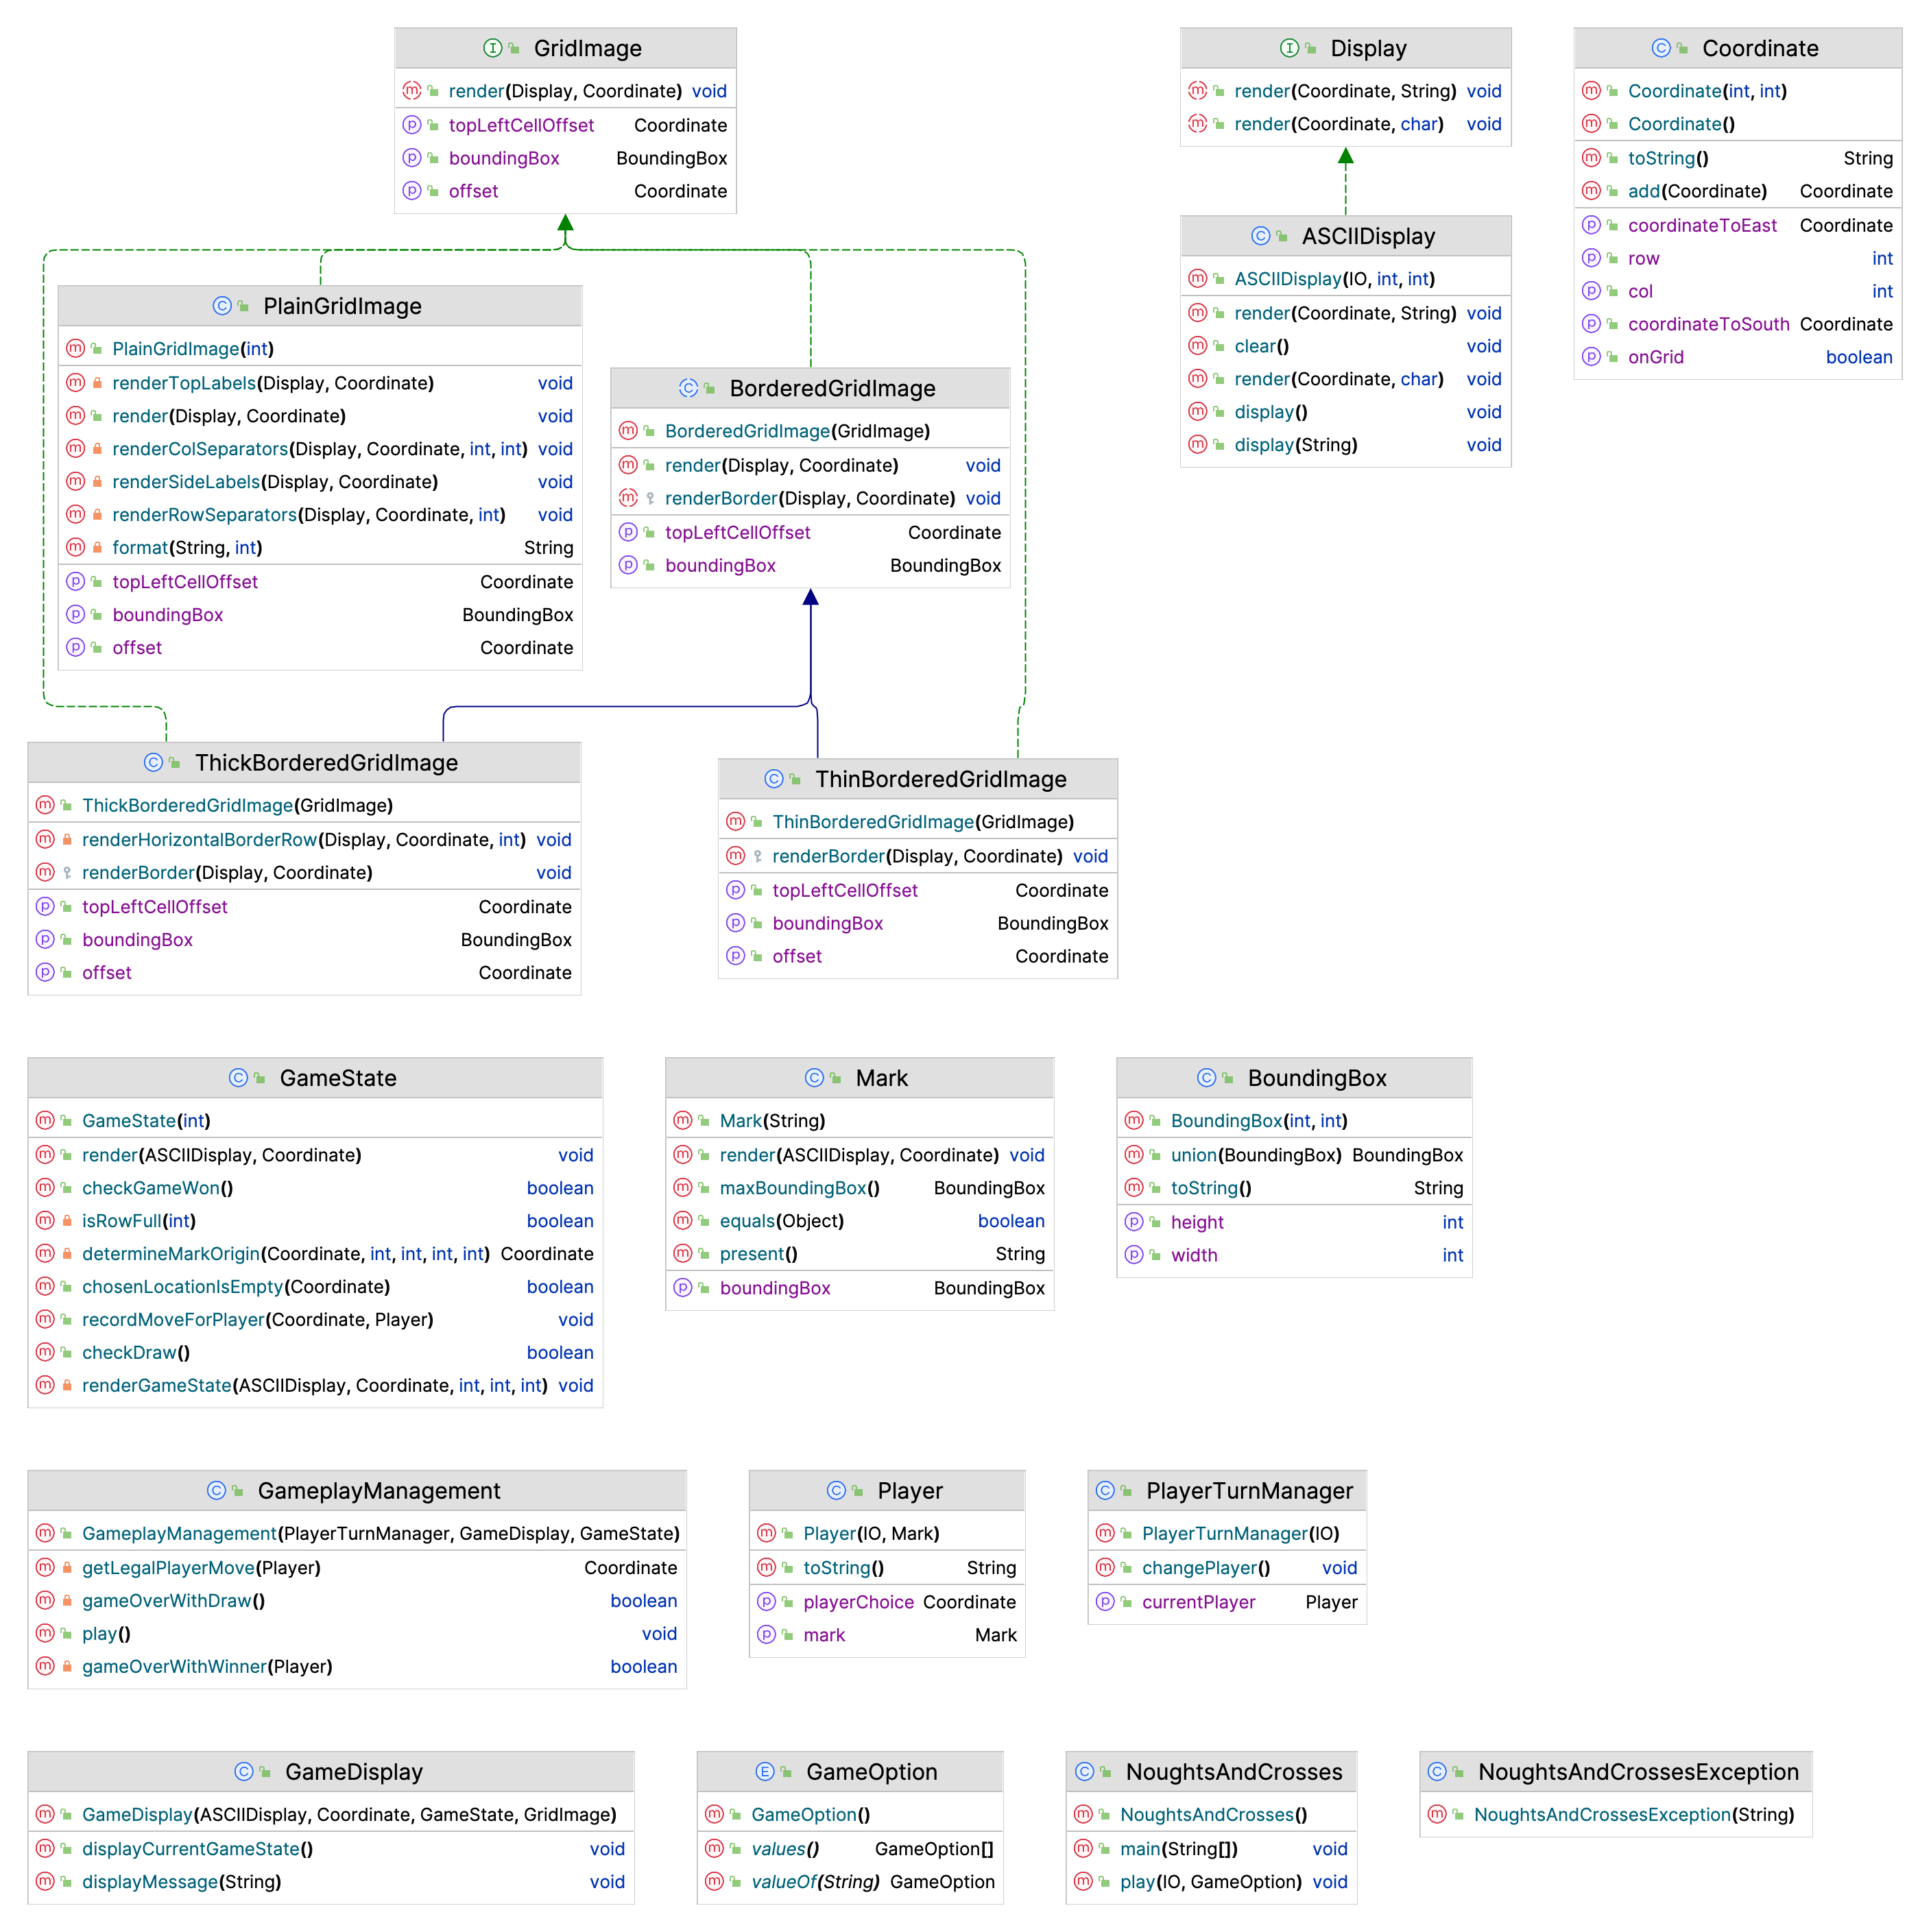
\includegraphics[width=18cm]{res/testuml.png}
    \caption{Test2 UML}
\end{figure}

在UML类图中单向关联用一个带箭头的直线表示。

双向关联就是双方各自持有对方类型的成员变量。在UML类图中,双向关联用一个不带箭头的直线表示。

自关联在UML类图中用一个带有箭头且指向自身的直线表示。

UML中聚合关系用带空心菱形和箭头的直线表示。聚合关系强调是“整体”包含“部分”,但是“部分”可以脱离“整体”而单独存在。比如汽车包含了发动机,而发动机脱离了汽车也能单独存在。

组合关系与聚合关系见得最大不同在于:这里的“部分”脱离了“整体”便不复存在,显然嘴是头的一部分且不能脱离了头而单独存在。在UML类图中,组合关系用一个带实心菱形和箭头的直线表示。

Driver的drive方法只有传入了一个Car对象才能发挥作用,因此我们说Driver类依赖于Car类。在UML类图中,依赖关系用一条带有箭头的虚线表示。

继承关系对应的是extend关键字,在UML类图中用带空心三角形的直线表示。

在UML类图中用带空心三角形的虚线表示实现关系。

\subsection{使用的设计模式}

\subsubsection{GridImage系列}

装饰器模式(Decorator Pattern): 这种设计模式允许在运行时向对象添加新功能,而不改变其结构。这种类型的设计模式属于结构模式,因为这种模式充当现有类的包装器。在这个例子中,BorderedGridImage 是一个装饰类,它增加了一个边框到基本的 GridImage 对象。ThickBorderedGridImage 和 ThinBorderedGridImage 是具体的装饰对象,它们分别添加了厚边框和薄边框。

组合模式(Composite Pattern): 通常用于表示对象的部分-整体层次结构。当你想要让客户端忽略单个对象与组合对象之间的差异时,就可以使用组合模式。GridImage 似乎是一个组合组件,它可以包含其他 GridImage 的实例,如 BorderedGridImage, ThickBorderedGridImage, 和 ThinBorderedGridImage。这些子类都继承自 GridImage 并可能有其自己的实现,形成了一个部分-整体的层次结构,这是组合模式的典型特征。

策略模式(Strategy Pattern): 这种模式涉及到算法的一个族系,能够相互替换,并让算法的变化独立于使用算法的客户。在这段代码中,GridImage 接口及其实现可能被视为策略模式的一部分,因为你可以根据需要在不同的 GridImage 实现之间进行切换,例如,你可以在 PlainGridImage、ThickBorderedGridImage 或 ThinBorderedGridImage 之间选择一个用于渲染。

\subsubsection{Display系列}

策略模式(Strategy Pattern):
在GameDisplay类中,GridImage和GameState作为参数传递到构造函数中,这表明了一种策略模式的使用。这个模式涉及将一系列算法(在这种情况下是渲染策略)定义为单独的类,然后在另一个类中使用它们。这允许算法的选择和变化不会影响到使用算法的类。在这里,GridImage和GameState可以是实现了特定接口的任何对象,GameDisplay不关心其内部工作方式,只是调用它们的render方法。这使得渲染逻辑可以在不更改GameDisplay类的情况下进行更改或扩展。

依赖注入(Dependency Injection):
GameDisplay类的构造函数接受ASCIIDisplay, Coordinate, GameState, 和GridImage对象作为参数,这是依赖注入的一种形式。依赖注入是一种允许类之间的依赖关系在运行时通过一个调用者来实现的设计模式。这增加了代码的模块化程度,使得单元测试更加容易,因为你可以传入模拟的依赖项来测试GameDisplay类的行为。
组合(Composition):

GameDisplay通过包含ASCIIDisplay, Coordinate, GameState, 和GridImage实例作为其属性,展示了组合的使用。组合是一种设计原则,它建议使用对象组合来实现新功能,而不是通过继承来扩展一个类的功能。GameDisplay类并没有从它的依赖项中继承功能,而是将它们组合在一起来实现新的功能。

\subsection{SOLID原则}

\subsubsection{GridImage系列 版本1}

单一职责原则 (Single Responsibility Principle, SRP):
GridImage 接口和它的实现类 PlainGridImage, BorderedGridImage, ThickBorderedGridImage, 和 ThinBorderedGridImage 都似乎遵循单一职责原则。每个类和接口都专注于网格图像的一个方面,无论是定义接口、处理无边框的图像、或是处理不同类型的边框。

开放封闭原则 (Open/Closed Principle, OCP):
这些类似乎也遵循开放封闭原则。例如,BorderedGridImage 是一个抽象类,可以被扩展来创建有不同边框的网格图像(如 ThickBorderedGridImage 和 ThinBorderedGridImage),而不需要修改现有代码。

里氏替换原则 (Liskov Substitution Principle, LSP):
从所给代码来看,子类似乎能够替代它们的基类。例如,任何需要 GridImage 的地方都可以使用 PlainGridImage、ThickBorderedGridImage 或 ThinBorderedGridImage,因为它们都遵循相同的接口。

接口隔离原则 (Interface Segregation Principle, ISP):
该原则建议将接口划分为更小的部分,避免强迫客户端实现它们不使用的方法。在这里,GridImage 接口似乎很简洁,只包含与网格图像相关的方法。不过,如果有些方法只适用于某些特定的图像,那么可能需要更多的接口来更好地隔离功能。

依赖反转原则 (Dependency Inversion Principle, DIP):
这些类似乎遵循依赖反转原则。例如,BorderedGridImage 依赖于 GridImage 接口而非 PlainGridImage 具体类。这意味着高级模块(如边框处理)不依赖于低级模块(如具体的网格图像实现),而是依赖于抽象。

\subsubsection{GridImage系列 版本2}

单一职责原则 (Single Responsibility Principle):
PlainGridImage 类似乎负责太多的呈现逻辑,如顶部标签、侧边标签、列分隔符和行分隔符的渲染。这可能违反了单一职责原则,因为如果要更改标签或分隔符的显示方式,你需要修改这个类。将这些职责分解为单独的类或方法可能会更好。

开放封闭原则 (Open/Closed Principle):
使用 GridImage 接口和如 BorderedGridImage 的抽象类,以及它们的具体实现如 ThickBorderedGridImage 和 ThinBorderedGridImage,项目似乎遵循了开放封闭原则。这是因为你可以通过创建新的 GridImage 实现来扩展网格的显示,而无需修改现有代码。

里氏替换原则 (Liskov Substitution Principle):
这些类似乎都遵循了里氏替换原则,因为它们都是从同一个接口 (GridImage) 继承而来,并且似乎可以互换使用,而不会影响程序的行为。

接口隔离原则 (Interface Segregation Principle):
GridImage 接口可能没有完全遵循接口隔离原则。这个接口为实现它的类施加了多种职责(获取边界框、获取偏移量、渲染等)。如果某个类只需要接口的部分功能,则该原则可能被违反。然而,在这个特定情况下,这似乎是必要的,因为所有的功能都是紧密相关的。

依赖倒置原则 (Dependency Inversion Principle):
类似乎都是依赖于 GridImage 这一抽象,而不是具体的实现,这是遵循依赖倒置原则的。然而,PlainGridImage 类直接与 Display 类交互,这意味着它依赖于一个具体的类而不是一个接口。如果 Display 是一个接口,并且具体的显示技术是它的实现,那么这将更好地遵循依赖倒置原则。

\subsubsection{Display系列}

S(Single Responsibility Principle,单一职责原则):
Display接口负责定义渲染方法,这是一个单一的职责。但是,它提供了两种不同的render方法,一种接受char,另一种接受String。这可能表明该接口承担了多重职责,尽管这两种方法都是渲染,但它们操作的数据类型不同。
GameDisplay类负责管理游戏的显示,包括渲染网格图像和游戏状态。这个类似乎有两个责任:管理游戏的显示和传递消息。虽然这些都与显示有关,但管理游戏状态的显示和通用消息传递可能被视为不同的职责。

O(Open/Closed Principle,开闭原则):
Display接口是开放的,因为可以实现新的Display类而无需修改接口。
GameDisplay类似乎对修改关闭,因为要改变显示的行为,你需要修改类的代码。然而,它对扩展是开放的,因为你可以通过传递不同的GridImage或GameState来改变渲染的外观和行为。

L(Liskov Substitution Principle,里氏替换原则):
从提供的代码中看不出违反此原则的明显迹象。然而,实际上是否符合此原则取决于实现Display接口的具体类的行为,以及如何使用GameDisplay类。

I(Interface Segregation Principle,接口隔离原则):
Display接口可能没有完全遵循接口隔离原则,因为它为不同类型的渲染(字符和字符串)定义了方法。如果某些类只需要一种渲染方法,这可能会迫使实现不需要的方法。

D(Dependency Inversion Principle,依赖倒置原则):
GameDisplay依赖于Display、GridImage和GameState的抽象,而不是具体实现,这符合依赖倒置原则。

\subsection{代码功能解析}

\subsubsection{Display 和 GameDisplay}

Display 是一个接口,用于定义渲染字符和字符串到某个坐标的方法。这是一个通用的、抽象级别的界面,可以被实现来显示游戏的不同部分。其定义了两个方法:
void render(Coordinate coord, char ch);:此方法接受一个 Coordinate 对象(代表在屏幕上的某个位置)和一个字符,然后将该字符渲染到指定的坐标。
void render(Coordinate coord, String str);:此方法与上一个类似,但它接受一个字符串而不是单个字符。这可以用于渲染字符串到特定的坐标。
由于 Display 只是一个接口,所以它不提供这些方法的具体实现。该接口的实现将依赖于具体的类(如可以将字符和字符串渲染到控制台、图形用户界面(GUI)或其他类型的显示)。

GameDisplay 是一个类,用于处理游戏的显示。它不直接实现 Display 接口,而是使用一个 Display 类型的对象(在这种情况下是 ASCIIDisplay 类型,该类型假定是 Display 接口的一个实现)。GameDisplay 负责管理和渲染游戏状态以及与玩家交互的其他界面元素。其成员变量包括:
\_origin:一个 Coordinate 对象,指示游戏渲染的起始点。
\_display:一个 ASCIIDisplay 对象,用于实际的渲染工作。假定 ASCIIDisplay 实现了 Display 接口。
\_gridImage:一个 GridImage 对象,代表游戏的网格。这可能是一个复杂的图像,表示游戏的棋盘。
\_gameState:一个 GameState 对象,维护游戏的当前状态(如哪个玩家的回合,棋盘上的哪些位置已经被占据等)。
该类具有以下方法:
public void displayCurrentGameState():此方法清除当前显示,重新渲染网格和游戏状态,然后显示它们。它使用 \_display、\_gridImage 和 \_gameState 成员变量来完成这些任务。
public void displayMessage(String message):此方法简单地在 \_display 上显示一条消息,可能是关于游戏状态的信息,例如“玩家X获胜”或“轮到玩家O”。
总的来说,Display 接口定义了渲染的基本合同,而 GameDisplay 类则利用这一合同来管理和显示游戏的具体状态和信息。

\subsection{对UML类图的解析}










\end{document}